% !TeX document-id = {e3a7ff19-e925-4f85-9d15-87fd720805e2}
% ******************************* PhD Thesis Template **************************
% Please have a look at the README.md file for info on how to use the template

\documentclass[a4paper,12pt,times,numbered,print,index,square, sort, numbers, authoryear]{Classes/PhDThesisPSnPDF}

% ******************************************************************************
% ******************************* Class Options ********************************
% *********************** See README for more details **************************
% ******************************************************************************

% `a4paper'(The University of Cambridge PhD thesis guidelines recommends a page
% size a4 - default option) or `a5paper': A5 Paper size is also allowed as per
% the Cambridge University Engineering Deparment guidelines for PhD thesis
%
% `11pt' or `12pt'(default): Font Size 10pt is NOT recommended by the University
% guidelines
%
% `oneside' or `twoside'(default): Printing double side (twoside) or single
% side.
%
% `print': Use `print' for print version with appropriate margins and page
% layout. Leaving the options field blank will activate Online version.
%
% `index': For index at the end of the thesis
%
% `draft': For draft mode without loading any images (same as draft in book)
%
% `abstract': To generate only the title page and abstract page with
% dissertation title and name, to submit to the Student Registry
%
% ************************* Custom Page Margins ********************************
%
% `custommargin`: Use `custommargin' in options to activate custom page margins,
% which can be defined in the preamble.tex. Custom margin will override
% print/online margin setup.
%
% *********************** Choosing the Fonts in Class Options ******************
%
% `times' : Times font with math support. ( The Cambridge University guidelines
% recommend using times)
%
% `fourier': Utopia Font with Fourier Math font
%
% `customfont': Use `customfont' option in the document class and load the
% package in the preamble.tex
%
% default or leave empty: `Latin Modern' font will be loaded.
%
% ********************** Choosing the Bibliography style ***********************
%
% `authoryear': For author-year citation eg., Krishna (2013)
%
% `numbered': (Default Option) For numbered and sorted citation e.g., [1,5,2]
%
% `custombib': Define your own bibliography style in the `preamble.tex' file.
% `\RequirePackage[square, sort, numbers, authoryear]{natbib}'
%
% **************************** Choosing the Page Style *************************
%
% `default (leave empty)': For Page Numbers in Header (Left Even, Right Odd) and
% Chapter Name in Header (Right Even) and Section Name (Left Odd). Blank Footer.
%
% `PageStyleI': Chapter Name next & Page Number on Even Side (Left Even).
% Section Name & Page Number in Header on Odd Side (Right Odd). Footer is empty.
%
% `PageStyleII': Chapter Name on Even Side (Left Even) in Header. Section Number
% and Section Name in Header on Odd Side (Right Odd). Page numbering in footer


% ********************************** Preamble **********************************
% Preamble: Contains packages and user-defined commands and settings

% \usepackage{picins,graphicx}
% ******************************************************************************
% ****************************** Custom Margin *********************************
% Add `custommargin' in the document class options to use this section
% Set {innerside margin / outerside margin / topmargin / bottom margin}  and
% other page dimensions
\ifsetMargin
\else
    \RequirePackage[left=37mm,right=30mm,top=35mm,bottom=30mm]{geometry}
    \setFancyHdr % To apply fancy header after geometry package is loaded
\fi

% *****************************************************************************
% ******************* Fonts (like different typewriter fonts etc.)*************

% Add `customfont' in the document class option to use this section
\ifsetFont
\else
    % Set your custom font here and use `customfont' in options. Leave empty to
    % load computer modern font (default LaTeX font).  
    \RequirePackage{libertine} 
\fi

% *****************************************************************************
% *************************** Bibliography  and References ********************

%\usepackage{cleveref} %Referencing without need to explicitly state fig /table

% Add `custombib' in the document class option to use this section
\ifsetBib % True, Bibliography option is chosen in class options
\else % If custom bibliography style chosen then load bibstyle here
    \RequirePackage[square, sort, numbers, authoryear]{natbib} % CustomBib
\fi

% changes the default name `Bibliography` -> `References'
\renewcommand{\bibname}{References}

% *****************************************************************************
% *************** Changing the Visual Style of Chapter Headings ***************
% Uncomment the section below. Requires titlesec package.

%\RequirePackage{titlesec}
%\newcommand{\PreContentTitleFormat}{\titleformat{\chapter}[display]{\scshape\Large}
%{\Large\filleft{\chaptertitlename} \Huge\thechapter}
%{1ex}{}
%[\vspace{1ex}\titlerule]}
%\newcommand{\ContentTitleFormat}{\titleformat{\chapter}[display]{\scshape\huge}
%{\Large\filleft{\chaptertitlename} \Huge\thechapter}{1ex}
%{\titlerule\vspace{1ex}\filright}
%[\vspace{1ex}\titlerule]}
%\newcommand{\PostContentTitleFormat}{\PreContentTitleFormat}
%\PreContentTitleFormat


% *****************************************************************************
% **************************** Custom Packages ********************************
% *****************************************************************************


% ************************* Algorithms and Pseudocode **************************

%\usepackage{algpseudocode} 


% ********************Captions and Hyperreferencing / URL **********************

% Captions: This makes captions of figures use a boldfaced small font. 
%\RequirePackage[small,bf]{caption}

\RequirePackage[labelsep=space,tableposition=top]{caption} 
\renewcommand{\figurename}{Fig.} %to support older versions of captions.sty


% ************************ Formatting / Footnote *******************************

%\usepackage[perpage]{footmisc} %Range of footnote options 


% ****************************** Line Numbers **********************************

%\RequirePackage{lineno}
%\linenumbers

% ************************** Graphics and figures *****************************
%\usepackage[help]{epspdfconversion}
\usepackage{epstopdf}
%\usepackage{rotating}
%\usepackage{wrapfig}
%\usepackage{float}
\usepackage{subfig} %note: subfig must be included after the `caption` package. 


% ********************************* Table **************************************

%\usepackage{longtable}
%\usepackage{multicol}
%\usepackage{multirow}
%\usepackage{tabularx}


% ***************************** Math and SI Units ******************************

\usepackage{amsfonts}
\usepackage{amsmath}
\usepackage{amssymb}
%\usepackage{siunitx} % use this package module for SI units


% ******************************************************************************
% ************************* User Defined Commands ******************************
% ******************************************************************************


% ********************** TOC depth and numbering depth *************************

\setcounter{secnumdepth}{2}
\setcounter{tocdepth}{2}

% ******************************* Nomenclature *********************************

% To change the name of the Nomenclature section, uncomment the following line

%\renewcommand\nomname{Symbols}


% ********************************* Appendix ***********************************

% The default value of both \appendixtocname and \appendixpagename is `Appendices'. These names can all be changed via: 

%\renewcommand{\appendixtocname}{List of appendices}

%\renewcommand{\appendixname}{Appndx}


\epstopdfsetup{outdir=Figs/PDF/}
\ifpdf
    \graphicspath{{Figs/Raster/}{Figs/PDF/}{Figs/}}
\else
    \graphicspath{{Figs/Vector/}{Figs/}}
\fi

% ************************ Thesis Information & Meta-data **********************
%% The title of the thesis
\title{A Fingertip Mechanical-Stress Detector using Chromatic Skin Information}
%\texorpdfstring is used for PDF metadata. Usage:
%\texorpdfstring{LaTeX_Version}{PDF Version (non-latex)} eg.,
%\texorpdfstring{$sigma$}{sigma}

%% The full name of the author
\author{Nayef Al-Saud}

%% Department (eg. Department of Engineering, Maths, Physics)
\dept{Department of Engineering}

%% University and Crest
\university{University of Cambridge}
\crest{
\includegraphics[width=0.25\textwidth]{Figs/University_Crest.eps}}

%% You can redefine the submission text:
% Default as per the University guidelines: This dissertation is submitted for
% the degree of Doctor of Philosophy
%\renewcommand{\submissiontext}{change the default text here if needed}

%% Full title of the Degree
\degree{Master of Philosophy in Engineering}

%% College affiliation (optional)
\college{Hughes Hall}

%% Submission date
\degreedate{17 February 2014}

%% Meta information
\subject{LaTeX} \keywords{{LaTeX} {MPhil Thesis} {Engineering} {University of
Cambridge}}



% ***************************** Abstract Separate ******************************
% To printout only the titlepage and the abstract with the PhD title and the
% author name for submission to the Student Registry, use the abstract option in
% the document class.

\ifdefineAbstract
 \includeonly{Abstract/abstract}
\else
\fi


% ******************************** Front Matter ********************************
\begin{document}


\frontmatter


\begin{titlepage}

\maketitle

\end{titlepage}

% ******************************* Thesis Dedidcation ********************************

\begin{dedication} 

I would like to dedicate this thesis to my little one. Let's never part again.

\end{dedication}


% ******************************* Thesis Declaration ********************************

\begin{declaration}

I hereby declare that except where specific reference is made to the work of others, the contents of this dissertation are original and have not been submitted in whole or in part for consideration for any other degree or qualification in this, or any other University. This dissertation is the result of my own work and includes nothing which is the outcome of work done in collaboration, except where specifically indicated in the text. This dissertation contains less than 15,000 words exclusive of footnotes, appendices and bibliography.

% Author and date will be inserted automatically from thesis.tex \author \degreedate

\end{declaration}


% ************************** Thesis Acknowledgements *****************************

\begin{acknowledgements}      


I would like to express my deepest gratitude to my supervisor, Prof. Roberto Cipolla, and my advisor, Dr. Joan Lasenby, for their guidance over the past two years, as well as their patience and understanding as I was learning the metaphorical computer vision ropes.
I would also like to acknowledge my colleague and friend Dr. Vijay Badrinarayanan, who was always around to offer advice, suggestions or simply a kind word whenever I was working too hard.
Most importantly, I woud like to thank my wonderful family and friends in Saudi, the states and elsewhere who supported me through the most difficult period of my life.



\end{acknowledgements}

% ************************** Thesis Abstract *****************************
% Use `abstract' as an option in the document class to print only the titlepage and the abstract.
\begin{abstract}
An efficient, lossless, chromatic color space employing a redistribution focused on an individual's particular chromatic skin statistics with application to the detection of blood flow. A color space transform is developed which avoids floating point operations, but which retains all the information contained in a source RGB image is developed and implemented. Several methods for feature detection, including a bespoke Canny edge detector which is designed to avoid some of the problems associated with feature detection in a chromatic space are implemented, and a proof of concept for a mechanical fingertip-stress detector is developed for an iOS device using the OpenCV computer vision library in C++ and shown to be not just possible, but effective on current devices.
\end{abstract}


% *********************** Adding TOC and List of Figures ***********************

\tableofcontents

\listoffigures

%\listoftables

% \printnomenclature[space] space can be set as 2.5cm between symbol and
% description
\printnomencl

% ******************************** Main Matter *********************************
\mainmatter

%*****************************************************************************************
%*********************************** First Chapter ***************************************
%*****************************************************************************************

\chapter{Motivation}  %Title of the First Chapter

\ifpdf
    \graphicspath{{Chapter1/Figs/Raster/}{Chapter2/Figs/PDF/}{Chapter2/Figs/}}
\else
    \graphicspath{{Chapter1/Figs/Vector/}{Chapter2/Figs/}}
\fi

Initially, this project was intended to be focused on skin detection and feature recognition for the potential application of hand tracking and posture prediction. However, it was quickly noticed that many authors were sticking to the RGB space, which suffers from disadvantages due to changes in lighting affecting the results. It was also noted that there seemed to be some significant disagreement over the methodology behind using a skin model~\cite{Shin2002a}~\cite{Sigal2000a}~\cite{Skarbek1994}~\cite{Soriano2000a}~\cite{Terrillon1999a}~\cite{Vezhnevets2003}~\cite{Brown2001a}. It appears that the reason many authors avoided luminosity-oriented color spaces was down to the computational intensity of performing the transform, the loss of information, and what seems like a rather perplexing issue to do with white-out, black-out and camera calibration. After reading over the literature, it was decided that two of these three issues were soluble, and the third was worthy of investigation.


The purpose of this project is to create a chromatic skin and feature detector for application in mobile devices. Using a given device's built-in CCD camera, objects with characteristics matching those of human skin are identified. This presents a number of challenges. Since we are trying to use the chromatic information of human skin to distinguish objects (e.g. hands, fingers) in a given scene, working in a chromatic space helps to simplify this problem. A chromatic space is a color space wherein the color information is laid out in as few dimensions as possible, with a separate dimension for luminosity --- the brightness information. Fundamentally, the issue with this is that CCD cameras capture information using RGB values in a spectrum which mixes the chromatic information with the luminosity. Separating this information is the first part of the challenge.

The second part of the challenge is, because we are searching for objects which exhibit certain chromatic characteristics, a statistical model must be developed and applied in order to characterize the objects as such.

The third and final challenge is developing efficient, discrete maths to perform the chromatic space rotation and statistical model efficiently enough such that all the chromatic information about the target object is retained, whilst all irrelevant information is discarded.

While several people have developed algorithms for skin detection, their focus has been squarely on detection rather than retention of information. For color spaces, Hue-Saturation based spaces, such as HSV, have been used due to the clear separation of the chromatic information and luminosity <Zarit and Sigal>. Simpler color spaces, such as Normalized RGB, have been used in video applications due to the demand of continuously processing image frames <Soriano>. As for gathering statistics, histogram thresholding <Soriano and Sigal> and Gaussian models using 2D Gaussians <Terrillon>, 3D Gaussians or multiple Gaussian clusters <Veshnevets> are among the most common models in practice <Shin>, though other models have been used to similar effect, such as the Self-Organizing Map (SOM) in <Brown>'s application. Additionally, practially every application uses double precision numbers in their transformations <Shin, Veshnevets and Terrillon>.

Regardless of the color spaces and statistical models used, all of these algoritms have the same fundamental approach: the image is transformed into some color space, and the statistical model is applied, resulting in a binary image which classifies whether any given pixel is skin. This information is then used as a mask and applied to the original image. This algorithm is fundamentally different to the one used for this project; the primary goal is to preserve information about the skin, as opposed to simply detecting whether a given object is skin or not. We process the image into a new chromatic space, then apply the statistical model, resulting in an image which contains all the chromatic and luminosity information about the skin within it, and information about non-skin areas is lost. 

We are preserving the information in a targeted way, reducing the overall infromation in the image whilst preserving the relevant information about the object we're interested in. This is a clear difference from the more common binary categorization approach, though it is possible to adapt our approach to the same process. However, as it stands, the entire process should be more efficient than the first step in a binary classifier, and should be faster than even moving to an HSV image.


\section{Choosing a Color Space}

As mentioned previously, one of the challenges facing this project is identifying a chromatic space in which the color information and luminosity from the raw RGB image can be separated, thereby simplifying the process of identification of human skin color. To this end, the most widely-used chromatic spaces in practical applications of skin color classification have been evaluated --- HSV, LAB and YCbCr --- all of which have a number of readily-available discrete implementations (\cite{Vezhnevets2003,Zarit1999a,Yang1997a,Brand2000a,Sigal2000a,Chai2000a,Phung2002a}).

Unlike RGB, the HSV color space makes a clear distinction between the chrominance (the "Hue" and "Saturation" channels) and the luminance (the "Value" channel), storing them separately (\cite{Vezhnevets2003,Sigal2000a}). However, the chromatic information in the Hue channel is expressed in polar coordinates, thereby necessitating a coordinate transform when converting from the raw image data. Given the nature of the algorithm outlined herein --- targeted preservation of information, as opposed to classification --- and the mechanical stress application of the algorithm, the computational cost of this transformation is undesirable.

LAB and YCbCr, on the other hand, not only explicity seperate the chrominance and luminance, the information is also expressed linearly (\cite{Vezhnevets2003,Poynton1997,Phung2002a}), thereby allowing for simple and quick conversion to and from the RGB space with no loss of information. However, while they appear to be perfectly suited for the purposes of this project, a number of issues arise when represented discretely. LAB, YCbCr and other such Hue-Saturation spaces all include implicit white-point correction in the readily-available implementations, which distorts the information from the raw image. Also, while the transform is reversible numerically, discrete data types are used in practical computer science applications, and in most implementations the output is the same data type as the input, resulting in some loss of information when the transform is applied. 

Furthermore, based on the skin statistics we have gathered --- which will be described in detail in the next chapter --- the entire region of skin color in the chromatic space can be expressed as a 2D Gaussian. Typically, this is a complex operation, but by aligning the chromatic axes of a Hue-Saturation space with the major and minor axes of the 2D Gaussian, it can be expressed as the product of two 1D Gaussians in each chromatic channel, thereby facilitating the application of the statistics. While it is possible to modify existing implementations of such Hue-Saturation spaces to achieve this, in light of the issues with white-point correction and loss of information due to discrete representation, it was decided that a bespoke chromatic space would be best suited for this project.






For the purposes of this project, a color space dedicated to human skin is necessary. When it comes to pattern recognition, it is beneficial to reduce the number of channels which the algorithm must process, as well as reducing the information density in those channels. It is also hoped that, in an appropriate color space, it will be a simple matter to separate the characteristics associated with saturation of tissue with blood, which changes under mechanical stress from the unchanging pigmentation of the cells (\cite{Stamatas2004}). Color spaces --- when they are normally defined --- are a combination of rotations, scaling and translations, while some (e.g. HSV (\cite{Vezhnevets2003, Zarit1999a} )) also perform a coordinate transform. The color space defined for this project is unusual in that it uses a non-linear redistribution of the values. It should be noted that this is not a pixel-based classifier (\cite{Jones2002}). However, seeing as the color space contains both the statistical information and the skin color information, it can be interpreted in a probabilistic way.

For the sake of comparison, the following four color spaces --- all of which have been used for skin detection (\cite{Vezhnevets2003,Zarit1999a,Yang1997a,Brand2000a,Sigal2000a,Chai2000a,Phung2002a}) --- have been evaluated for the purposes of this project.

\subsection{LAB}\label{sec:LAB}

The LAB color space's perceptual uniformity makes it well-suited for skin detection, as the human eye can perceive practically any change in its values (\cite{Vezhnevets2003,Poynton1997}). However, the Gaussian distribution of the skin is not positioned on the axis, which makes applying the statistics troublesome.

\subsection{RGB}\label{sec:RGB}

The RGB color space, while widely used, is perhaps the most ill-suited color space for skin detection, as it can't make a distinction between chrominance and luminance, as discussed by ~\cite{Vezhnevets2003,Brand2000a}. That said, its ubiquity in cameras --- which are designed to capture images which, to us, appear to be an accurate representation of physical reality despite the opposite being true --- makes it a necessary color space to work in. The advantage to using it is simply the fact that it is a straightforward, raw output from the camera.

\subsection{HSV}\label{sec:HSV}

Unlike RGB, the HSV color space makes a clear distinction between the chrominance (the "Hue" and "Saturation" channels) and the luminance (the "Value" channel), storing them separately (\cite{Vezhnevets2003,Sigal2000a}). This makes HSV a popular choice for skin segmentation, but it's difficult to control any information loss during the transform due to its non-linearity (\cite{Poynton1997}).

\subsection{YCbCr}\label{sec:YCbCr}

This color space bears similarities to the LAB and HSV spaces in that it explicitly separates the chrominance and the luminance. The luminosity (or "luma") channel "Y" is a weighted sum of the RGB values (\cite{Poynton1997,Phung2002a}), while the chrominance channels "Cb" and "Cr" contain the color difference between Y and the red and blue components of RGB, respectively (\cite{Vezhnevets2003}). Also like LAB, it is not oriented such that the Gaussian distribution is situated along the axis. In fact, there is little distinction between the two spaces aside from the orientation in the chromatic portion of the space.

The main issue with using these color spaces is the lack of control over information flow upon transformation and the clear mathematical statement of the transformation in terms of rotation, scaling and translation. Therefore, the construction of a new color space is necessary.

Reasons for LAB: because LXY/LAB spaces all include implicit white-point correction in the readily-available implementatons, so there's no control over that. They all compress the information back into--they all use the same data type, the whole bit about "yes, the transform is reversible, but not really, because we're using discrete data types and most implementations the output is the same data type as the input. You can't fit a box into another box at an angle; the box needs to be big enough for it or it will lose the information. So they all implicitly do that. The second point is because we're using a 2D gaussian which, if we align the major and minor axes, then it's just a 1D gaussian in two of the chrom channels. So applying the stats is better. 

So!

1. Distortion from implicit white-point corrections.

2. Loss of information.

3. To facilitate the application of the stats.



\section{Physiology Study}\label{sec:PhysiologyStudy}

Right, we're going from chemistry to computer science, yeah? This is the point, we're--we're going from physicalto virtual how we want to say it?

The response spectra is how you turn wavelength into RGB. 'cause that's weird. We have a physical quantity, the energy of light, and we have to turn it into three numbers. Weird, huh? That depends upon the measuring device, so if that's an eye, it has a certain response based on the chemistry of the cones, yeah? In our retina. The retina produces that signal, yeah? But there are only three different types of cones which produce that kind of signal--well, we have cones and rods so it's kinda like RGBa, so we detect color and luminosity seperately, but whatever, in terms of color our cones produce RGB. CCDs are based on that and they produce RGB signals, but the absorption-- to do that, we take the wavelength which is generally in nanometers, and a response function, which is dimensionless, it's just the response--y'know the output, one for blue one for green one for red. The red one has, um, for eyes it has a weird bump, and a secondary bump there--the point is that there are a load of different response spectra. So we have a function for R G and B, depending on-- keep it simple, we're not making a big deal about it-- it is whatever it is. And what we have here in mathemativa (wavelength.nb) if you look at mathematica's graphical rep it simulates the red bump of the eye response, and we'll come back to that.

Now, also, we have the absorption spectra. We have some skin, and we have our chromophores. We have hemoglobin, hemo-oxy and three forms of melanin but we have the data for two. But they're good enough; they give us an in. There are other chromophores that can be included which are breakdown products of blood, the stuff which makes bruises green, a variety of chemicals, but we'll restrict ourselves to these major components, the major chromophores in the skin. Now, the chromophores and the ones that contribute to diffusion. Now, chromophores are for absorption and the rest is dispersed (scattered). The point is that we are--we've consistently called it re-emission. ANYWAY, it's what comes out of the surface. So as absorption goes up, remittance goes down. Then there's blood constants, molar mass (very heavy; 64kg/mo), a--nevermind looking at mathematica file now.

If we wanna make this quick, we gotta get the raw data from CCD and process it, but they all look weird; lots of variability, but they're corrected to match the more sensible one, hence all the correction.




The image captured by a CCD camera is designed to fool the human eye. In physical reality, light reaching the sensor spans full spectral range. In the human eye --- and in the camera --- the diversity of chromatic information is lost by representing the spectrum as a combination of three chromatic Gaussians, as can be seen in Figure~\ref{fig:spectrum}.

\begin{figure}[h!]
  \centering
    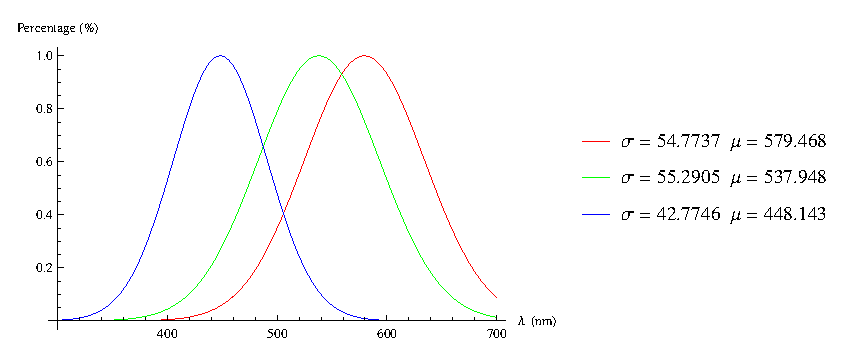
\includegraphics[width=\textwidth]{Chapter2/Figs/spectrum.eps}
    \caption{Human eye representation of the color spectrum.}  \label{fig:spectrum}
\end{figure}

Human skin is made up of two layers, each with its own optical properties: the surface layer --- the "epidermis" --- and the "dermis," the vascular structure underneath in which the blood vessels, lymphatic vessels and other such fibroblast structures can be found (~\cite{Stamatas2004}). The molecules which make up these layers make an important contribution to skin color. The most significant of these are melanin --- which is found in the epidermis --- and oxy-hemoglobin and deoxy-hemoglobin --- both of which reside in the dermis. Melanin is the main spectral absorber in the epidermis and the greatest contributor to the visual perception of surface skin color; it features a monotonic increase toward short wavelengths on its spectral absorption curve in the visible, approaching linear in the region 600-750 nm (~\cite{Stamatas2004,Kollias1995,Zonios2001}). Oxy-hemoglobin and deoxy-hemoglobin are actually different states of the same molecule --- hemoglobin --- which is found in the dermal blood supply. The molecule's chromophoric state is dependent upon whether it is delivering oxygen molecules to the tissues; it exists as oxy-hemoglobin if it is delivering oxygen and deoxy-hemoglobin if it isn't. The redness of skin in the areas where hemoglobin is found is due to the molecule's absorption of incident light (~\cite{Kollias1995}). It should be noted that each form of hemoglobin has its own characteristic absorption profile; oxy-hemoglobin's maxima on the absorption curve can be found at 415, 540 and 577 nm, whereas deoxy-hemoglobin's are located at 430 and 555 nm.

Seeing as the chromophores' absorption characteristics are expressed as wavelengths, it should be possible to turn a wavelength into a point in a color space. The absorption spectra is a complete description of the material. As such, it can be used to show what the material would look like under any lighting condition. The white light spectrum as perceived by the human eye can be represented using RGB Gaussian waveforms by turning the absorption spectra into a scattering spectra and representing it in terms of the RGB Gaussians. Through the use of an additive process based on Grassman's law, which states that, if the sample color is a combination of two monochromatic colors, then the value found by the observer for each monochromatic base color from the sample color will be the sum of each sample base color of the two monochromatic colors observed separately, we can find points in the R, G and B channels in the RGB color space for the three chromaphores (~\cite{MIHAI2007}).

The equivalent RGB points for the colors of the absorption peaks can be calculated as follows:

\begin{equation}
\begin{array}{cc}
 \{0.6\, -0.0136667 (\lambda -380),0,0.02 (\lambda -380)+0.39\} & \lambda \geq 380.\land \lambda \leq 410. \\
 \{0.19\, -0.00633333 (\lambda -410),0,1\} & \lambda \geq 410.\land \lambda \leq 440. \\
 \left\{0,\frac{\lambda -490}{50}+1,1\right\} & \lambda \geq 440.\land \lambda \leq 490. \\
 \left\{0,1,\frac{510-\lambda }{20}\right\} & \lambda \geq 490.\land \lambda \leq 510. \\
 \left\{\frac{\lambda -580}{70}+1,1,0\right\} & \lambda \geq 510.\land \lambda \leq 580. \\
 \left\{1,\frac{640-\lambda }{60},0\right\} & \lambda \geq 580.\land \lambda \leq 640. \\
 \{1,0,0\} & \lambda \geq 640.\land \lambda \leq 700. \\
 \{0.008125 (780-\lambda )+0.35,0,0\} & \lambda \geq 700.\land \lambda \leq 780. \\
\end{array}
 \\
\end{equation}

If the respective color is shined on a molecule with these properties, it will absorb them. To convert this into a scattering spectrum, spectrum of the incident light must be taken, subtracting the amount that is absorbed. Assuming a uniform line, the process is not unlike flipping the waveform on its Y axis.

\begin{figure}[h!]
  \centering
    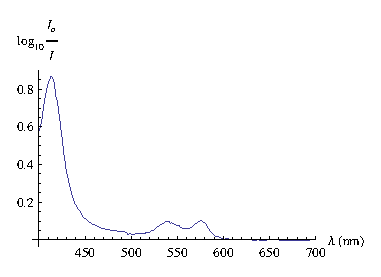
\includegraphics[width=0.45\textwidth]{Chapter2/Figs/absOxyHemo.eps}
    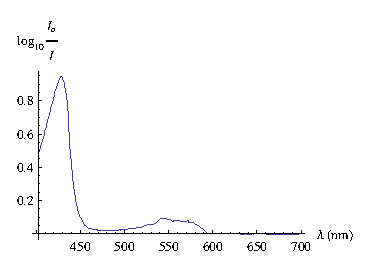
\includegraphics[width=0.45\textwidth]{Chapter2/Figs/absDeoxyHemo.eps}
    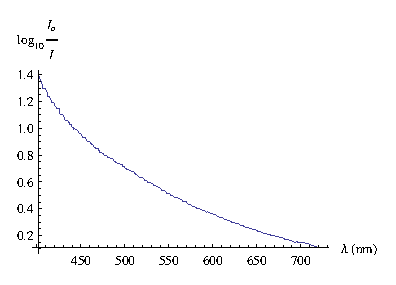
\includegraphics[width=0.45\textwidth]{Chapter2/Figs/absMelanin.eps}
    \caption{Oxy-hemoglobin, deoxy-hemoglobin and melanin absorption characteristics.}  \label{fig:abs}
\end{figure}

The scattering spectra needs to be represented in a three-function Gaussian basis. We will take the maximum values of these and make a quick transform of the scattering spectra, giving a color value for the molecules and their relative positions in the space. The scattering spectra are presented in Figure~\ref{fig:scat}.

\begin{figure}[h!]
  \centering
    
\includegraphics[width=0.45\textwidth]{Chapter2/Figs/scatOxyHemo.eps}
    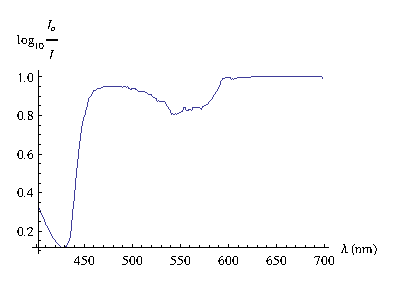
\includegraphics[width=0.45\textwidth]{Chapter2/Figs/scatDeoxyHemo.eps}
    
\includegraphics[width=0.45\textwidth]{Chapter2/Figs/scatMelanin.eps}
    \caption{Oxy-hemoglobin, deoxy-hemoglobin and melanin scattering spectra.}  \label{fig:scat}
\end{figure}

Finally, we perform a color matching operation based on the CIE 1931 standard observer piecewise function to complete the transformation.

\begin{figure}[h!]
  \centering
    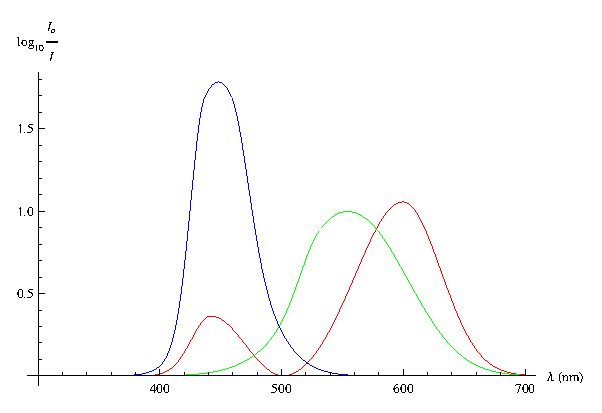
\includegraphics[width=\textwidth]{Chapter2/Figs/colorBasis.eps}
    \caption{Final skin chromophore positions.}  \label{fig:colorBasis}
\end{figure}

We have a function for the light source, but we will make the crude assumption of an equal amount of all wavelengths. This is sufficient for the purposes of this project.

%********************************** %First Section  **************************************
%\section{Motivation} %Section - 1.1 





%********************************** %Second Section  *************************************
%\section{Overview of Color Spaces} %Section - 1.2


%********************************** % Third Section  *************************************
%\section{Where does it come from?}  %Section - 1.3 
%\label{section1.3}



%*****************************************************************************************
%*********************************** Second Chapter **************************************
%*****************************************************************************************

\newcommand{\unitDst}{\text{uDst}} % Destination in the unit range 0:1
\newcommand{\uDst}{\unitDst}       % Destination in the unit range 0:1
\newcommand{\intDst}{\text{iDst}}  % Destination in the integer range dstMin:dstMax
\newcommand{\iDst}{\intDst}        % Destination in the integer range dstMin:dstMax
\newcommand{\dstMax}{\text{dstMax}}      % Destination integer range maximum
\newcommand{\dstMin}{\text{dstMin}}      % Destination integer range mimimum
\newcommand{\dstRange}{\text{dstRange}}  % Destination integer range
\newcommand{\discreteDst}{\widetilde{\uDst}}   % Destination found using the discretized transformation matrix
\newcommand{\dDst}{\discreteDst}               % Destination found using the discretized transformation matrix
\newcommand{\delDst}{\delta\uDst}              % Error in the Destination found using the discretized transformation matrix

\newcommand{\unitT}{\text{uT}}             % Rotated values in the unit range 0:1
\newcommand{\uT}{\unitT}                   % Rotated values in the unit range 0:1
\newcommand{\intT}{\text{iT}}              % Rotated values in the integer range tMin:tMax
\newcommand{\iT}{\intT}                    % Rotated values in the integer range tMin:tMax
\newcommand{\tMax}{\text{tMax}}            % Rotated values integer range maximum
\newcommand{\tMin}{\text{tMin}}            % Rotated values integer range mimimum
\newcommand{\tRange}{\text{tRange}}        % Rotated values integer range
\newcommand{\discreteT}{\widetilde{\uT}}   % Rotated values found using the discretized transformation matrix
\newcommand{\dT}{\discreteT}               % Rotated values found using the discretized transformation matrix
\newcommand{\delT}{\delta\uT}              % Error in the Rotated values found using the discretized transformation matrix

\newcommand{\unitSrc}{\text{uSrc}}       % Source in the unit range 0:1
\newcommand{\uSrc}{\unitSrc}             % Source in the unit range 0:1
\newcommand{\intSrc}{\text{iSrc}}        % Source in the integer range srcMin:srcMax
\newcommand{\iSrc}{\intSrc}              % Source in the integer range srcMin:srcMax
\newcommand{\srcMax}{\text{srcMax}}      % Source integer range maximum
\newcommand{\srcMin}{\text{srcMin}}      % Source integer range mimimum
\newcommand{\srcRange}{\text{srcRange}}  % Source integer range

\newcommand{\unitX}{\text{uX}}       % Source in the unit range 0:1
\newcommand{\uX}{\unitX}             % Source in the unit range 0:1
\newcommand{\intX}{\text{iX}}        % Source in the integer range xMin:xMax
\newcommand{\iX}{\intX}              % Source in the integer range xMin:xMax
\newcommand{\xMax}{\text{xMax}}      % Source integer range maximum
\newcommand{\xMin}{\text{xMin}}      % Source integer range mimimum
\newcommand{\xRange}{\text{xRange}}  % Source integer range

\newcommand{\unitY}{\text{uY}}       % Destination in the unit range 0:1
\newcommand{\uY}{\unitY}             % Destination in the unit range 0:1
\newcommand{\intY}{\text{iY}}        % Destination in the integer range yMin:yMax
\newcommand{\iY}{\intY}              % Destination in the integer range yMin:yMax
\newcommand{\yMax}{\text{yMax}}      % Destination integer range maximum
\newcommand{\yMin}{\text{yMin}}      % Destination integer range mimimum
\newcommand{\yRange}{\text{yRange}}  % Destination integer range

\newcommand{\unitR}{\text{uR}}
\newcommand{\uR}{\unitR}
\newcommand{\intR}{\text{iR}}
\newcommand{\iR}{\intR}
\newcommand{\discreteR}{\widetilde{\uR}}
\newcommand{\dR}{\discreteR}
\newcommand{\delR}{\delta\uR}
\newcommand{\rRange}{\text{rRange}}  % the discretization of the rotation matrix


\chapter{Color Spaces and Information Storage for Computer Vision Processing} \label{sec:Chap2}

\epstopdfsetup{outdir=Chapter2/Figs/PDF/}
\ifpdf
    \graphicspath{{Chapter2/Figs/Raster/}{Chapter2/Figs/PDF/}{Chapter2/Figs/}}
\else
    \graphicspath{{Chapter2/Figs/Vector/}{Chapter2/Figs/}}
\fi


\section{Constructing a New Color Space}\label{sec:ConstructingANewColorSpace}

In order to construct a new color space, we need to consider the coordinate system of the new color space, the orientation of the new color space, and the fidelity of the discrete representation of the axes.

The first consideration is most easily decided; because there's little obvious advantage otherwise, we choose a Cartesean coordinate system as this allows for a straightforward transformation involving only rotation, translation and scaling. Because we're interested in the color information in the image, it's useful to design the color space so there is a luminosity axis. This choice determines two of three rotational degrees of freedom, as will be discussed below.

As for the discrete representation of the axes, it's desired that all the information captured pertaining to a hand should be preserved; all other information is irrelevant. However, here we'll consider only the effect of a rotation and scaling on the discrete representation.


\subsection{Camera RGB and Normalization for Discrete Range}\label{sec:CameraRGB}

Due to the iPhone hardware being locked down at the application level, we do not have access to the raw camera feed. We do, however, have access to the post-processing (color-rebalanced and white-point-corrected) 8-bit RGB image data.

Because we're searching for particular points in the real color space --- which, being a continuous function, is infinite dimensional --- there is a possibility in the future that larger multi-channel color spaces will be much more common, such as the 8-channel color spaces currently in development. Though most such cameras are primarily designed for post-production editing for still pictures and film (e.g. changing the lighting independent of the scene), as well as visual effects, the possibilities for computer vision are exciting. However, computer vision tasks are computationally intensive, and more often than not require operation in real time, so there is a natural inclination to shy away from large data sets in practical computer vision applications; many tasks are done in grayscale or single-channel processing to expedite the process.

As such, there is a need to develop techniques which keep the relevant information while quickly and efficiently discarding the irrelevant information. This is true for the RGB space at the moment, and the aim of this first part of the work.


\subsection{Rotation Matrix}\label{sec:RotationMatrix}
Any rotation about an axis can be represented by a 3x3 square matrix in a 3D space. Since they are invertible, they're guaranteed to be non-singular. However, as there are many ways in which to rotate an object from one position to another, or use a combination of different rotations to get to the same point, they aren't necessarily unique. For this application, we require rotation about three different axes, which can be expressed thus:


\begin{alignat}{1}
R_x(\theta) &= \begin{bmatrix}
1 & 0 & 0 \\
0 & \cos \theta &  -\sin \theta \\[3pt]
0 & \sin \theta  &  \cos \theta \\[3pt]
\end{bmatrix} \\[6pt]
R_y(\theta) &= \begin{bmatrix}
\cos \theta & 0 & \sin \theta \\[3pt]
0 & 1 & 0 \\[3pt]
-\sin \theta & 0 & \cos \theta \\
\end{bmatrix} \\[6pt]
R_z(\theta) &= \begin{bmatrix}
\cos \theta &  -\sin \theta & 0 \\[3pt]
\sin \theta & \cos \theta & 0\\[3pt]
0 & 0 & 1\\
\end{bmatrix}
\end{alignat}


Any rotation which orients the RGB color space such that one of the new axes lies along the luminosity direction is sufficient; a rotation which aligns the L axis along the luminosity direction is produced by a rotation of $\frac{\pi}4$ about the red (\textbf{R}) axis, followed by a rotation of $\arctan{\frac{1}{\sqrt{2}}}$ about the green (\textbf{G}) axis. This leaves one free rotational degree of freedom about the L axis. The resulting rotation matrix is given by:

\begin{equation}
R_{xyz}(\theta) =
\left(
\begin{array}{ccc}
 \frac{1}{\sqrt{3}} & \frac{1}{\sqrt{3}} & \frac{1}{\sqrt{3}} \\
 -\sqrt{\frac{2}{3}} \sin \left(\theta +\frac{\pi }{6}\right) & \sqrt{\frac{2}{3}} \cos (\theta ) & -\sqrt{\frac{2}{3}} \sin \left(\frac{\pi }{6}-\theta \right) \\
 -\sqrt{\frac{2}{3}} \cos \left(\theta +\frac{\pi }{6}\right) & -\sqrt{\frac{2}{3}} \sin (\theta ) & \sqrt{\frac{2}{3}} \cos \left(\frac{\pi }{6}-\theta \right) \\
\end{array}
\right)
\end{equation}


Where $\theta$ is the remaining rotational degree of freedom.

Using the standard rotation matrices, we get a luminosity axis which spans the range $0:\sqrt{3}$. However, the length of the two remaining axes are dependent on the value of $\theta$ used. This is a problem because, ultimately, we want the axes to fit in a range of an appropriate data type. It would be more useful to have a matrix which provided the specified rotation and scaled the axis to known lengths. In the case of the luminosity, this is straightforward; simply divide by $\sqrt{3}$. In the case of the other two axes, we need an explicit form for the lengths of the axis resulting from the rotation.

Because the absolute values of the axes in the color space have no meaning, we're only interested in the position along the axis relative to its start and end, equivalent to talking about the position in the axis relative to $0:1$, compared to about $0:255$ in unsigned, 8-bit integers. The upside is that if we're rotating the cube about its corner, we're interested in the minimum and maximum values possible along the new axis direction, which will correspond to a corner of the RGB cube. With the L axis aligned along the luminosity direction, the range of the L axis is 0 to $\sqrt{3}$. The x and y axes are symmetrical, spanning a range centered on 0. The range of their values is dependent upon the remaining degree of freedom.

We need to know, in each of the axes, how far out each point is. Because we're effectively rotating a hexagon, whatever the answer is, we know the function is going to be periodic, repeating every $\frac{\pi}{3}$ radians, so we only have to solve it in the $0:\frac{\pi}{3}$ region and then generalize. First we take the coordinates of the RGB cube and perform the rotation to find the values in the new color space.


\begin{multline}\label{eq:YabCube}
  R_{xyz}(\theta)\cdot\left(
\begin{array}{cccccccc}
 0 & 1 & 1 & 0 & 0 & 0 & 1 & 1 \\
 0 & 0 & 1 & 1 & 1 & 0 & 0 & 1 \\
 0 & 0 & 0 & 0 & 1 & 1 & 1 & 1 \\
\end{array}
\right) = \\
\resizebox{\textwidth}{!}{%
$\displaystyle
\left(
\begin{array}{cccccccc}
 0 & \frac{1}{\sqrt{3}} & \frac{2}{\sqrt{3}} & \frac{1}{\sqrt{3}} & \frac{2}{\sqrt{3}} & \frac{1}{\sqrt{3}} & \frac{2}{\sqrt{3}} & \sqrt{3} \\
 0 & -\sqrt{\frac{2}{3}} \sin \left(\theta +\frac{\pi }{6}\right) & \sqrt{\frac{2}{3}} \sin \left(\frac{\pi }{6}-\theta \right) & \sqrt{\frac{2}{3}} \cos (\theta ) & \sqrt{\frac{2}{3}} \sin \left(\theta +\frac{\pi }{6}\right) & -\sqrt{\frac{2}{3}} \sin \left(\frac{\pi }{6}-\theta \right) & -\sqrt{\frac{2}{3}} \cos (\theta ) & 0 \\
 0 & -\sqrt{\frac{2}{3}} \cos \left(\theta +\frac{\pi }{6}\right) & -\sqrt{\frac{2}{3}} \cos \left(\frac{\pi }{6}-\theta \right) & -\sqrt{\frac{2}{3}} \sin (\theta ) & \sqrt{\frac{2}{3}} \cos \left(\theta +\frac{\pi }{6}\right) & \sqrt{\frac{2}{3}} \cos \left(\frac{\pi }{6}-\theta \right) & \sqrt{\frac{2}{3}} \sin (\theta ) & 0 \\
\end{array}
\right)$}
\end{multline}


The extent of the new axis is found by taking the maximum and minimum values of each row i.e. the extreme corner positions relative to each new axis. An additional symmetry of the hexagonal projection of the RGB cube allows us to say that whatever functional form is taken by one of the $\theta$ dependant ranges the other can be found by a simple phase shift. So recognising that the minimum value is simply $-1$ times the maximum we have simplified the problem to solving

\begin{equation}\label{eq:AxisRangeMinMax}
 \max\left(\pm\frac{\sin (\theta )}{\sqrt{6}}\pm\frac{\cos (\theta )}{\sqrt{2}}, \pm\sqrt{\frac{2}{3}} \sin (\theta ) \right) \quad \text{Where} \quad 0\leq \theta \leq \frac{\pi}{3}
\end{equation}

A graphical representation of the problem can be seen in Figure~\ref{eq:YabCube}.

\begin{figure}[h!]
  \centering
    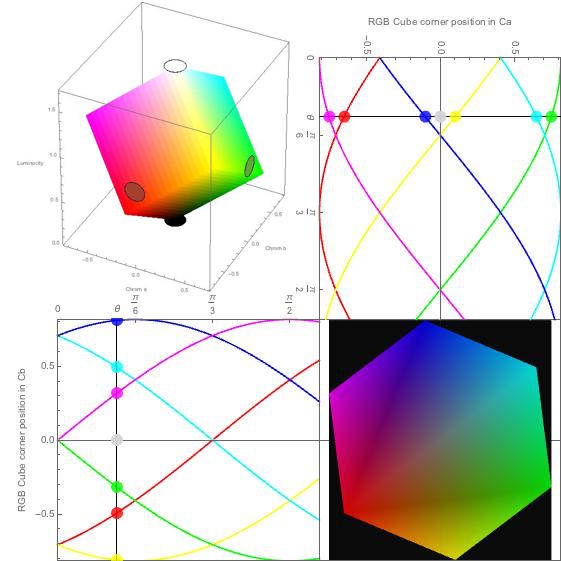
\includegraphics[width=\textwidth]{Chapter2/Figs/CornersOf_theRGBCube.jpg}
    \caption{Evaluation of the color space problem. The cube in the top-left shows the positions of the axes in the rotated space; the white and black disks on the vertical axis represent the white point and black point of the luminosity axis, and the other disks represent the ends of the chromatic axes \textbf{Ca} and \textbf{Cb}. The graphs in the top-right and bottom-left show the positions of the corners of the RGB cube relative to the chromatic axes \textbf{Ca} and \textbf{Cb}. The bottom-right graphic shows the RGB cube viewed down the luminosity axis. The graphics were generated by interactive code written in Mathematica. The value of $\theta$ was an arbitrary value from a snapshot taken from the interactive graphic.}\label{fig:YABCubeEval}
\end{figure}

In the range $0:\frac{\pi}{3}$, both sin and cos are positive, therefore the axis ranges are given by the following:

\begin{tabular}{|c|c|c|}
  \hline
  % after \\: \hline or \cline{col1-col2} \cline{col3-col4} ...
    & Min & Max \\ \hline
  L & \(0\) & \(\sqrt{3}\) \\
  Ca & \(- \sqrt{\frac{2}{3}} \cos \left(\frac{\pi }{6}-(\left(\theta -\frac{\pi }{6}\right) \bmod \frac{\pi }{3})\right) \)&\( \sqrt{\frac{2}{3}} \cos \left(\frac{\pi }{6}-(\left(\theta -\frac{\pi }{6}\right) \bmod \frac{\pi }{3})\right) \)\\
 Cb & \(-\sqrt{\frac{2}{3}} \cos \left(\frac{\pi }{6}-(\theta  \bmod \frac{\pi }{3})\right) \)&\( \sqrt{\frac{2}{3}} \cos \left(\frac{\pi }{6}-(\theta  \bmod \frac{\pi }{3})\right) \)\\
  \hline
\end{tabular}

The lengths of the axis after rotation are given by:
\begin{equation}\label{eq:L}
\mathbf{L}(\theta) = \left(
\begin{array}{c}
\sqrt{3} \\
 \sqrt{\frac{2}{3}} \sin \left(\widetilde{\vartheta}\right) + \sqrt{2} \cos \left(\widetilde{\vartheta}\right) \\  
\sqrt{\frac{2}{3}} \sin \left(\widetilde{\theta}\right) + \sqrt{2} \cos \left(\widetilde{\theta}\right) 
\end{array}
\right)
\quad \text{where}  \quad 
\begin{array}{c}
\widetilde{\theta} = \theta  \bmod \frac{\pi }{3} \\ 
\widetilde{\vartheta} = \left(\theta - \frac{\pi }{6}\right) \bmod \frac{\pi }{3}
\end{array}
\end{equation}

It is convenient to produce a transformation which will result in axes of known length. Because the rotation cannot include a translation, we desire a transformation matrix which will result in the ranges $0:1$, -$\frac{1}2:\frac{1}2$, and -$\frac{1}2:\frac{1}2$. Such a transformation is easily obtained by multiplying the rotation matrix by a diagonal matrix with the reciprocal of the maximums found above placed along the diagonal. This will scale each axis to a unit length.

The normalized 'rotation' matrix is given by:


\begin{equation}\label{eq:NormRxyz3}
 \overline{R}_{xyz}(\theta) =
\left(
\begin{array}{c}
 \frac{1}{\sqrt{3}}  \\
 \frac{1}{L_2(\theta)} \\
 \frac{1}{L_3(\theta) }  \\
\end{array}
\right)
\bigotimes
R_{xyz}(\theta)
\end{equation}

This matrix is no longer technically a rotation matrix as its inverse is no longer equal to its transpose. It now equal to:

\begin{equation}\label{eq:NormRxyz3Inverse}
 \overline{R}_{xyz}^{-1}(\theta) =
 R_{xyz}(\theta)^{T} \bigotimes
\left(
\begin{array}{ccc}
 \frac{1}{\sqrt{3}}  &
 \frac{1}{L_2(\theta)} &
 \frac{1}{L_3(\theta) }
\end{array}
\right)
\end{equation}

\subsection{Representing the Rotation}

The final piece of the metaphorical jigsaw is to add the capability to deal with the machine handling of the numerics. The transforms as defined above assume the capacity to represent the resulting numbers. Unfortunately, on a device, the numerics are not handled in such a pure way and --- whilst we are uninterested in the information overflow outside the destination representation --- this can cause instabilities in a practical implementation. In the development of the algorithm, it is therefore necessary to define these bounds. In the unit space, these bounds have already been defined by Equation~\ref{eq:L}; so long as the axis length can be represented on the device between these bounds, then overflow and underflow can be dealt with using a simple conditional statement.

It is significantly advantageous to perform calculations using integer types, particularly given that the input and output types are integers with small ranges, meaning it's possible to construct algorithms which avoid conversion to floating point operations. To this end, we wish to determine the most efficient internal representation for the transformation.

We have a well-defined distribution which represents the desired conservation of information, which itself is represented by the distribution function in the unit ranges. Each of these unit ranges is discretized into steps of $\frac{1}{\srcRange}$ and $\frac{1}{\tRange}$. The question then is to what degree of accuracy do we need to represent the internal numerics? If we represent the transformation in a discrete type $\discreteR$, we can express the problem in terms of the largest perturbation which can be made to the transformation without affecting the result.


\begin{equation}\label{eq:lxyPixel}
\begin{aligned}
\uR  \cdot \uSrc &= \uT  &\text{let} \quad \uR &= \dR + \delR \\
(\discreteR + \delR)  \cdot \uSrc &= \discreteT + \delT \\
\text{therefore if } \discreteR \cdot \uSrc &= \discreteT & \text{then}\quad \delR  \cdot \uSrc = \delT
\end{aligned} 
\end{equation}

The continuous rotation $\uR$ can be expressed as the sum of its discrete representation $\dR$ with discretization factor and the correction $\delR$. The elements of the discrete rotation can be expressed as rational fractions.

\begin{eqnarray}\label{eq:dRRange}
\discreteR = \dfrac{int(\uR \cdot \rRange)}{\rRange}\quad where\quad int(1.5) = 1, int (-1.5) = -1\\
therefore\quad \dfrac{-1}{\rRange} < \delR  < \dfrac{1}{\rRange}
\end{eqnarray}

It should be noted that --- unlike the source type \uSrc --- the perturbation can be negative. The definition of the function $int$ results in the sign of the perturbation matching the sign of the discertized transformation matrix. We must therefore consider both the maximum and minimum of $\delT$. As $0 \le\uSrc \le 1$ the extrema of $\delT$ are found where $\uSrc$ is a vector with elements of 0 and 1. If the matrix is decomposed into a sum of positive and negative elements $\delT = \delT_+ + \delT_-$ then the extrema are given by $\max(\delT_+ \cdot \mathbf{1})$ and $\min(\delT_- \cdot \mathbf{1})$. Where the elements are positive or negative is determined by the sign of the elements in the rotation matrix $\uR$. If we were to scale the entire matrix evenly then the top row would dominate as it is always positive and the necessary discrete representation would be characterised by $\rRange = 3 \; \tRange$. This would, however, necessitate the matrix being stored in a data type with at least 2 more bits than the source type. As the source type will be fully utilised in all but the most unusual applications this will result in a doubling of the bit depth for the matrix and a quadrupling of the bit depth for the working calculation. We will therefore consider each row individually and because the transformation is scaled by row as described previously. The second and third rows each sum to zero $\uR \mathbf{1} = [\sqrt{3},0,0]$ allowing us to state that each of the rows has one element of the opposite sign to the other two elements. The discretization for the second and third rows then only requires $\rRange = 2 \; \tRange$. It is also possible to pull out common factors from the rows to facilitate the reduction in the required representation.

\begin{equation}
\uR(\theta) =
\left(
\begin{array}{c}
 \frac{1}{\sqrt{3}} \\
 \sqrt{\frac{2}{3}}  \\
 \sqrt{\frac{2}{3}} \\
\end{array}
\right) \bigotimes
\left(
\begin{array}{ccc}
 1 & 1 & 1 \\
 -\sin \left(\theta +\frac{\pi }{6}\right) &  \cos (\theta ) &  \sin \left(\theta -\frac{\pi }{6}\right) \\
 -\cos \left(\theta +\frac{\pi }{6}\right) & - \sin (\theta ) & \cos \left(\theta -\frac{\pi }{6}\right) \\
\end{array}
\right)
\end{equation}
The rotation matrix may now be adequately represented in a discrete range of $\rRange = 2 \tRange$ with all elements taking values between -1 and 1 because the top row consists entirely of integers negating the necessity to represent the elements as rational fractions.

One further optimization is possible if we consider the redistribution of the values which is performed after the rotation. Not all information contained in the source is of equal value, so an error introduced by using a less accurate discretization of the rotation may well be mitigated by the subsequent redistribution. Halving the discrete range will introduce errors of at most 1 for some of the pixel values. In general, using $\rRange = 2^{1-n} \; \tRange$ will introduce a maximum error of $\frac{2^n -1}{\tRange}$ into the resulting colorspace. We must now establish which elements are affected.

The sign of the rotation matrix is given by

\begin{equation}
\left(
\begin{array}{ccc}
1
 &
1
 &
1
 \\
\begin{cases}
   1 & \frac{5 \pi }{6}<\theta <\frac{11 \pi }{6} \\
 -1 & \left\lgroup \begin{array}{c} 0\leq \theta <\frac{5 \pi }{6} \\ \frac{11 \pi }{6}<\theta <2 \pi  \end{array} \right.\\
\end{cases}
 &
\begin{cases}
 1   & \left\lgroup \begin{array}{c} 0\leq \theta <\frac{\pi }{2} \\ \frac{3 \pi }{2}<\theta <2 \pi  \end{array} \right.\\
 -1 & \frac{\pi }{2}<\theta <\frac{3 \pi }{2} \\
\end{cases}
 &
\begin{cases}
 1 & \frac{\pi }{6}<\theta <\frac{7 \pi }{6} \\
 -1 & \left\lgroup \begin{array}{c}  0\leq \theta <\frac{\pi }{6} \\ \frac{7 \pi }{6}<\theta <2 \pi  \end{array} \right.\\
\end{cases}
 \\

\begin{cases}
 1 & \frac{\pi }{3}<\theta <\frac{4 \pi }{3} \\
 -1 & \left\lgroup \begin{array}{c} 0 \leq \theta <\frac{\pi }{3} \\ \frac{4 \pi }{3}<\theta <2 \pi \end{array} \right. \\
\end{cases}
 &
\begin{cases}
 1 & \pi <\theta <2 \pi  \\
 -1 & 0<\theta <\pi  \\
\end{cases}
 &
\begin{cases}
   1 & \left\lgroup \begin{array}{c} 0\leq \theta <\frac{2 \pi }{3} \\ \frac{5 \pi }{3}<\theta <2 \pi  \end{array} \right.\\
 -1 & \frac{2 \pi }{3}<\theta <\frac{5 \pi }{3} \\
\end{cases}
 \\
\end{array}
\right)
\end{equation}

We are interested in which elements in each row share the same sign, as these will determine the pixel values which contribute to the error. If we find the intersecting conditions and flip the sign where there are two negative elements, the following is found
\begin{equation}
\begin{cases}
 \left(
\begin{array}{ccc}
 1 & 1 & 1 \\
 0 & 0 & 0 \\
 0 & 0 & 0 \\
\end{array}
\right) & \theta =\frac{\pi }{6}\lor \theta =\frac{\pi }{2}\lor \theta =\frac{5 \pi }{6}\lor \theta =\frac{7 \pi }{6}\lor \theta =\frac{3 \pi }{2}\lor \theta =\frac{11 \pi }{6} \\
 \left(
\begin{array}{ccc}
 1 & 1 & 1 \\
 -1 & 1 & 1 \\
 -1 & 1 & 1 \\
\end{array}
\right) & \frac{\pi }{6}<\theta <\frac{\pi }{2}\lor \frac{7 \pi }{6}<\theta <\frac{3 \pi }{2} \\
 \left(
\begin{array}{ccc}
 1 & 1 & 1 \\
 1 & -1 & 1 \\
 1 & -1 & 1 \\
\end{array}
\right) & 0\leq \theta <\frac{\pi }{6}\lor \frac{5 \pi }{6}<\theta <\frac{7 \pi }{6}\lor \frac{11 \pi }{6}<\theta <2 \pi  \\
 \left(
\begin{array}{ccc}
 1 & 1 & 1 \\
 1 & 1 & -1 \\
 1 & 1 & -1 \\
\end{array}
\right) & \frac{\pi }{2}<\theta <\frac{5 \pi }{6}\lor \frac{3 \pi }{2}<\theta <\frac{11 \pi }{6} \\
\end{cases}
\end{equation}
So for a pixel $\{R,G,B\}$  % \parpic{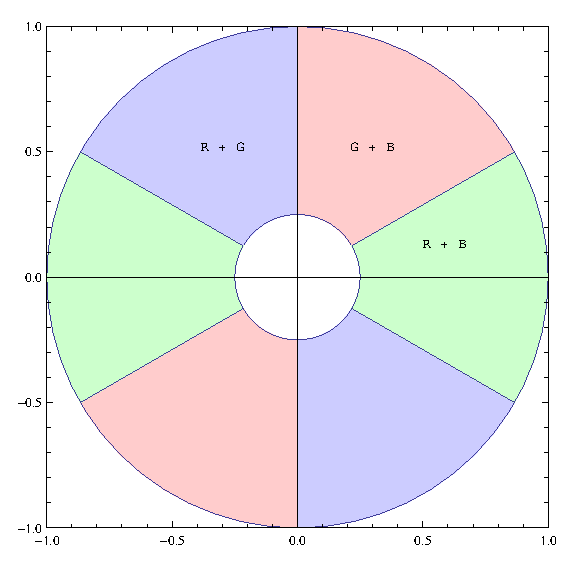
\includegraphics[width=100mm]{Chapter2/Figs/ErrorIntheRotation.eps}}
\begin{equation}\label{eq:errorFreeConditions}
\raisebox{-22mm}{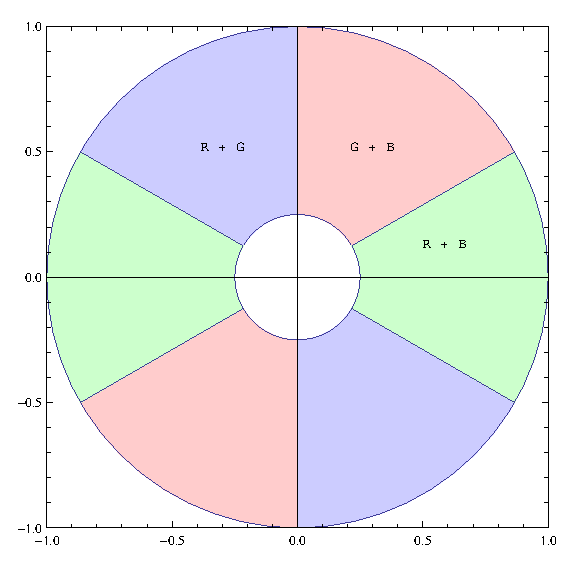
\includegraphics[width = 44mm]{Chapter2/Figs/ErrorIntheRotation.eps}}\begin{cases}
 G + B < 1 & \frac{\pi }{6}<\theta <\frac{\pi }{2}\lor \frac{7 \pi }{6}<\theta <\frac{3 \pi }{2} \\
 R + B < 1 & 0\leq \theta <\frac{\pi }{6}\lor \frac{5 \pi }{6}<\theta <\frac{7 \pi }{6}\lor \frac{11 \pi }{6}<\theta <2 \pi  \\
 R + G < 1 & \frac{\pi }{2}<\theta <\frac{5 \pi }{6}\lor \frac{3 \pi }{2}<\theta <\frac{11 \pi }{6} \\
\end{cases}
\end{equation}

where 1 indicates that the element shares its sign with another element in the same row and -1 indicates the opposite. One channel from the source can be left error free whilst the sum of the other two must be less than one. this divides the color space in two. If the portion of the source which is to be preserved better than in a 2:1 ratio lies entirely within the error free half then the rotation matrix can be stored in the same data type as the source itself. This can be designed as it does not matter if we rotate the colorspace in $\frac{\pi}{2}$ steps.


\begin{equation}
\intR =
\text{int}\left(
\left(
\begin{array}{c}
 1 \\
 2^{1-n_2} \; \tRange_2\\
 2^{1-n_3} \; \tRange_3 \\
\end{array}
\right) 
\bigotimes
\left(
\begin{array}{ccc}
 1 & 1 & 1 \\
 -\sin \left(\theta +\frac{\pi }{6}\right) &  \cos (\theta ) &  \sin \left(\theta -\frac{\pi }{6}\right) \\
 -\cos \left(\theta +\frac{\pi }{6}\right) & - \sin (\theta ) & \cos \left(\theta -\frac{\pi }{6}\right) \\
\end{array}
\right)
\right)
\end{equation}

\begin{equation}
\widehat{R}_{xyz}(\theta,\mu,\sigma) =
\left(
\begin{array}{c}
 \frac{\min\left\{\Delta(\mu_1,\sigma_1), 1 \right\}}{\sqrt{3}}  \\
 \sqrt{\frac{2}{3}} \frac{\min\left\{\Delta(\mu_2,\sigma_2), 1 \right\} }{2^{1-n_2} \; \tRange_2} \\
 \sqrt{\frac{2}{3}} \frac{\min\left\{\Delta(\mu_3,\sigma_3), 1 \right\}}{2^{1-n_3} \; \tRange_3} \\
\end{array}
\right) 
\bigotimes
\intR 
\end{equation}

using $\tRange(\theta,\mu,\sigma) = \min\left\{\Delta(\mu,\sigma), 1 \right\} \srcRange \mathbf{L}(\theta) $
\begin{equation}
\widehat{R}_{xyz}(\theta,\mu,\sigma) =
\left(
\begin{array}{c}
 \frac{\min\left\{\Delta(\mu_1,\sigma_1), 1 \right\}}{\sqrt{3}}  \\
 \sqrt{\frac{2}{3}} \frac{1}{2^{1-n_2} \; \srcRange \text{L}_2(\theta)} \\
 \sqrt{\frac{2}{3}} \frac{1}{2^{1-n_3} \; \srcRange \text{L}_3(\theta)} \\
\end{array}
\right) 
\bigotimes
\intR 
\end{equation}

\begin{equation}
\widehat{R}_{xyz}(\theta,\mu,\sigma) =
\left(
\begin{array}{c}
\min\left\{\Delta(\mu_1,\sigma_1), 1 \right\} \\
\min\left\{\Delta(\mu_2,\sigma_2), 1 \right\}  \\
\min\left\{\Delta(\mu_3,\sigma_3), 1 \right\}  \\
\end{array}
\right)
\bigotimes
\left(
\begin{array}{c}
 \frac{1}{\sqrt{3}} \\
 \sqrt{\frac{2}{3}}  \\
 \sqrt{\frac{2}{3}} \\
\end{array}
\right) \bigotimes
\left(
\begin{array}{c}
 1 \\
 \frac{1}{2^{1-n_2} \; \tRange_2} \\
 \frac{1}{2^{1-n_3} \; \tRange_3} \\
\end{array}
\right) 
\bigotimes
\text{int}\left(
\left(
\begin{array}{c}
 1 \\
 2^{1-n_2} \; \tRange_2\\
 2^{1-n_3} \; \tRange_3 \\
\end{array}
\right) 
\bigotimes
\left(
\begin{array}{ccc}
 1 & 1 & 1 \\
 -\sin \left(\theta +\frac{\pi }{6}\right) &  \cos (\theta ) &  \sin \left(\theta -\frac{\pi }{6}\right) \\
 -\cos \left(\theta +\frac{\pi }{6}\right) & - \sin (\theta ) & \cos \left(\theta -\frac{\pi }{6}\right) \\
\end{array}
\right)
\right)
\end{equation}

All that remains is to determine if the statistics allow for a reduced representation of the rotation. An equtaion for the boundary of the one to one fidelity region must be found in the source color space and then checked against the conditions given above \ref{eq:errorFreeConditions}. 

\section{Preservation of Color Information}\label{sec:PreservationOfColorInformation}

The goal of the algorithm is to preserve all the information captured by the camera which relates to skin whilst discarding as much of the irrelevant information as possible. Given that edges and features often present as shadows and highlights, all the information captured in terms of luminosity will be regarded as relevant information, at least as far as the manipulation of individual pixel values is concerned. Considering the chromatic information, the importance of the pixel value will be directly determined by the Gaussian distribution found previously.

Knowing the range of values produced by the rotation allows us to scale the transformation to fit into the range of the destination data type. If we have RGB pixel values in a given machine data type, the amount of information contained in each of those channels is equal to the number of values accessible in that data type. For example: for 8-bit, unsigned integers, there are 256 possible values. After a rotation, we are interested in the amount of information which lies along the new axes. This is found simply by multiplying the range of the source data type by the length of the new axes found for the unit cube. To preserve all the information captured, we would therefore have to use a larger data type to store the new values. We are, however, only interested in a small region in the chromatic space. The question is, then, how to preserve the relevant information in a way consistent with the significance indicated by the Gaussian distribution found previously.


None of the rotated axes have lengths less than 1 for the unit RGB cube. For this reason we've written redistribution functions which perform any necessary type conversion whilst preserving the information in a controlled way; we can keep the information where it's needed and discard it where it's irrelevant. So although this is strictly beyond the normal meaning of a color space conversion, it is addressing a connected issue and belongs in the conversion. In terms of optimization, it is also the most efficient place in the code in which to perform this adjustment, allowing us to --- for the sake of example --- discard the details of the colors of a duck's feathers whilst keeping the hues and tones of human skin.

We can use a function to redistribute the information contained on the longer axis onto the shorter axis, which can be expressed in the discrete representation of that axis necessitated by internal integer data types. There are three ways in which to implement the redistribution functions:

\subsection{Partition}\label{sec:Partition}

The most straightforward redistribution method is to simply preserve the information in a 1-to-1 fashion within a region. The region can be defined in terms of the skin color distribution Gaussian by specifying a significance level in terms of the variance or the standard deviation.

\subsection{Linear}\label{sec:Linear}

A slightly more sophisticated method is to use a linear redistribution. A linear distribution is equivalent to partitioning given a unit gradient. However, a linear redistribution function allows for the possibility of data compression. So then, in the case where the region of interest contains more information than can be expressed in the destination data type, a linear distribution function allows an even compression of the information from source to destination. ~\cite{Lee2002}

\subsection{ERF (Gaussian Error Function)}\label{sec:ERF}

The integral of the cumulative Gaussian (i.e. Error Function) allows the redistribution of the information on the axis in a way which selectively preserves the information about a point on the axis (i.e. the mean of the Gaussian), and then progressively discard the information as it falls into the tails of the Gaussian. So, it provides a non-linear distribution of the information. The Gaussian can be seen as describing our interest in the information contained along the axis, so it's logical to use the error function to redistribute the information. The disadvantage of this is simply the computational effort involved in generating the error function.

The error function distribution is mathematically correct, being directly related to the Gaussian fit. Computationally, there are two considerations: the numerical representation, and performance. The discrete representation of the numerics means that --- for a significant number of possible distributions --- distributing using the error function has little to no advantage (or indeed difference) from using a linear distribution.

Considering the preservation of information captured, mappings with a gradient greater than 1 are undesirable because they preserve all the information whilst being informatically wasteful in that there are functionally inaccessible discrete values in the destination range. Our stated aim is to preserve the information in the image pertaining to human skin; unevenly distributing this information across a discrete data type is not only wasteful in terms of memory, but also of processing resources because subsequent processing routines will treat the data as if it has a higher fidelity than it actually does.

To construct a distribution function, we first need to describe the relationship of the error function to the Gaussian fit, and then produce a function with the appropriate range and domain. For a Gaussian fit with an amplitude A, a mean of $\mu$, and a standard deviation of $\sigma$, where $\mu$ and x lie in a source range $\xRange$ from $\xMin$ to $\xMax$. The cumulative distribution is found by integrating from $\xMin$ to the point x, as can be seen in (\ref{eq:ErfDefinition}):

\begin{equation}\label{eq:ErfDefinition}
  \int _{\xMin}^{\text{x}} A \frac{e^{-\frac{(t-\mu )^2}{2 \sigma ^2}}}{\sqrt{2 \pi } \sigma }dt=\frac{1}{2} A \left(\text{erf}\left(\frac{\text{x}-\mu }{\sqrt{2} \sigma }\right)-\text{erf}\left(\frac{\xMin-\mu }{\sqrt{2} \sigma }\right)\right)
\end{equation}

The Gaussian distribution and the cumulative distribution are shown in Figure~\ref{fig:ErrorFunctionGraph} for some values chosen for illustrative purposes. All that is required now is to fix the range $\yMin$ to $\yMax$ for the domain $\xMin$ to $\xMax$.

\begin{figure}[h!]
  \caption{Error function.}  \label{fig:ErrorFunctionGraph}
  \centering
    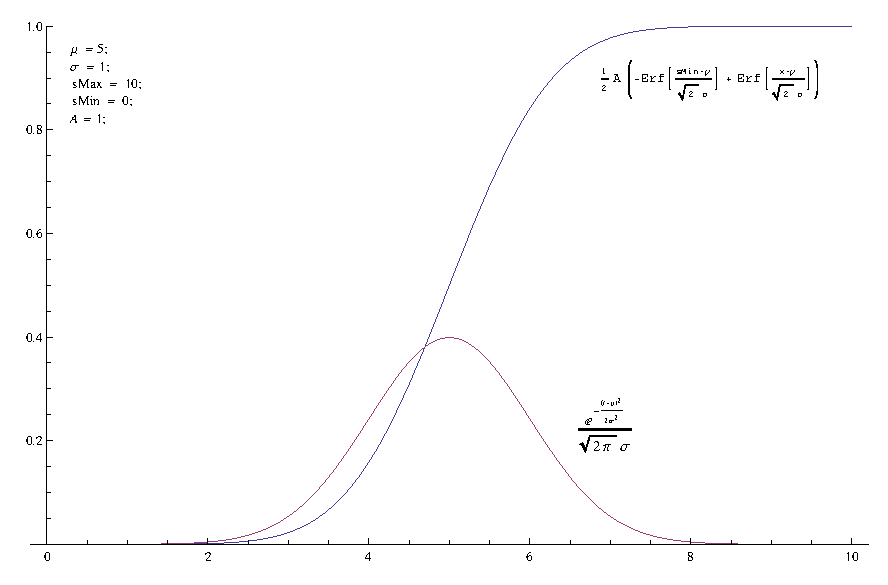
\includegraphics[width=\textwidth]{Chapter2/Figs/errorFunction.eps}
\end{figure}

First, we determine the maximum value taken in the domain. This is simply found by evaluating the function at $\xMax$. It should be noted that --- if the Gaussian distribution is well-contained in the source domain --- the maximum value should be equal to the amplitude. For the sake of simplicity, we'll ignore the amplitude of the fitted Gaussian found previously as it is not relevant to the design of the redistribution function. So, to fix the range of the distribution function, we first scale to the range $0:1$ by simply dividing through by the maximum value, and then re-scale to the destination range $\yRange = \yMax - \yMin$ and shift by $\yMin$.

\begin{equation}\label{eq:disFunction}
  dis(x) = \frac{(\yRange) \left(\text{erf}\left(\frac{x-\mu }{\sqrt{2} \sigma }\right)-\text{erf}\left(\frac{\xMin-\mu }{\sqrt{2} \sigma }\right)\right)}{\text{erf}\left(\frac{\xMax-\mu }{\sqrt{2} \sigma }\right)-\text{erf}\left(\frac{\xMin-\mu }{\sqrt{2} \sigma }\right)}+\yMin
\end{equation}

Mathematically, this distribution function~(\ref{eq:disFunction}) achieves all the stated objectives. However, on a device we are dealing with discrete numerics and limited processing power, so further analysis is required. Where we're using a discrete domain and range, the distribution is usefully divided into three characteristic behaviors:  where it is constant, where it preserves all the information, and where it selectively preserves information. Looking at the distribution, this divides the source domain into five regions: two where it is effectively constant, two where it is selective, and one region around the mean where it preserves all the information. In order to design an efficient algorithm, it is useful to identify the boundaries of these five regions.

First, we need to identify where the distribution is effectively constant. This can be found by solving the following equation in the region and domain $0 \le x \le 1$ and then generalized to the specific discrete numerics:

\begin{equation}\label{eq:0to1}
 \frac{\text{erf}\left(\frac{\mu }{\sqrt{2} \sigma }\right)+\text{erf}\left(\frac{x-\mu }{\sqrt{2} \sigma }\right)}{\text{erf}\left(\frac{\mu }{\sqrt{2} \sigma }\right)-\text{erf}\left(\frac{\mu -1}{\sqrt{2} \sigma }\right)}=\text{dL} \quad \text{where} \quad \text{dL} = \left\{ \frac{1}{\yRange}, 1 - \frac{1}{\yRange} \right\}
\end{equation}


The solution is found for the source domain in the range $0:1$ as:


\begin{equation}\label{eq:LowHigh}
 x = \sqrt{2} \sigma  \text{erf}^{-1}\left((\text{dL}-1) \text{erf}\left(\frac{\mu }{\sqrt{2} \sigma }\right)-\text{dL} \; \text{erf}\left(\frac{\mu -1}{\sqrt{2} \sigma }\right)\right)+\mu
\end{equation}

To find the region where all the information in the source domain is preserved, we differentiate the distribution and solve for where the gradient is equal to the destination range over the source range. This corresponds to the point at which a unit change in the source produces a unit change in the destination range:

\begin{equation}\label{eq:Boundaries}
\frac{\sqrt{\frac{2}{\pi }} e^{-\frac{(x-\mu )^2}{2 \sigma ^2}}}{\sigma  \left(\text{erf}\left(\frac{\mu }{\sqrt{2} \sigma }\right)-\text{erf}\left(\frac{\mu -1}{\sqrt{2} \sigma }\right)\right)}=\frac{\yRange}{\xRange}
\end{equation}

Rearranging for $x$, we find:

\begin{equation}\label{eq:PreservedRegion}
 x=\mu \pm \sigma  \sqrt{-2 \log \left(\sigma  \left(\text{erf}\left(\frac{\mu }{\sqrt{2} \sigma }\right)-\text{erf}\left(\frac{\mu -1}{\sqrt{2} \sigma }\right)\right)\right)+2 \log \left(\frac{\xRange}{\yRange}\right)+\log \left(\frac{2}{\pi }\right)}
\end{equation}

We now have equations which gives us the four points in the source domain which mark the boundaries of the five characteristic regions. The equations are valid in the unit source domain $0:1$. It is a simple matter to scale and shift these values to give the points in a more general source domain.


\begin{equation}
\begin{aligned}
\Sigma^- &= \text{erf}\left(\frac{\mu -1}{\sqrt{2} \sigma }\right) &
 \Sigma^+ &= \text{erf}\left(\frac{\mu }{\sqrt{2} \sigma }\right) &
  \text{dL} &= \frac{1}{\yRange} &
  \kappa &= \frac{\yRange}{\xRange} 
\end{aligned}
\end{equation}

\begin{equation}\label{eq:PreservedRegionGen}
\begin{aligned}
\Lambda^-(\mu,\sigma) &= \xMin + \xRange\left( \mu - \sigma  \sqrt{-2 \log \left(\sigma  \left(\Sigma^+-\Sigma^-\right)\right) - 2 \log \left(\kappa\right)+\log \left(\frac{2}{\pi }\right)}\right) \\
\Lambda^+(\mu,\sigma) &= \xMin + \xRange \left(\mu + \sigma  \sqrt{-2 \log \left(\sigma  \left(\Sigma^+-\Sigma^-\right)\right)-2 \log \left(\kappa\right)+\log \left(\frac{2}{\pi }\right)}\right)
\end{aligned}
\end{equation}

\begin{equation}\label{eq:LowHighGen}
\begin{aligned}
\lambda^+(\mu,\sigma)  &=  \xMin + \xRange \left( \sigma \sqrt{2}  \text{erf}^{-1}\left((\text{dL}-1) \Sigma^- -\text{dL} \; \Sigma^+ \right)+\mu \right) \\
\lambda^-(\mu,\sigma)  &=  \xMin + \xRange \left( \sigma \sqrt{2} \text{erf}^{-1}\left((\text{dL}-1) \Sigma^+-\text{dL} \; \Sigma^-\right)+\mu \right)
\end{aligned}
\end{equation}



\begin{figure}[h!]
  \centering
    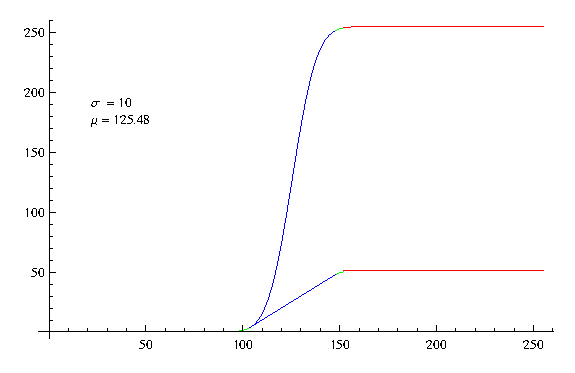
\includegraphics[width=0.49\textwidth]{Chapter2/Figs/partitionSmooth2.eps}
    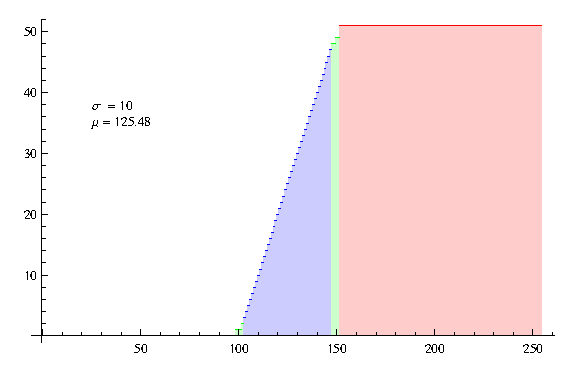
\includegraphics[width=0.49\textwidth]{Chapter2/Figs/partitionColor2.eps}
    \caption{Linear partition approximation.}  \label{fig:Partition}
\end{figure}

\begin{figure}[h!]
  \centering
    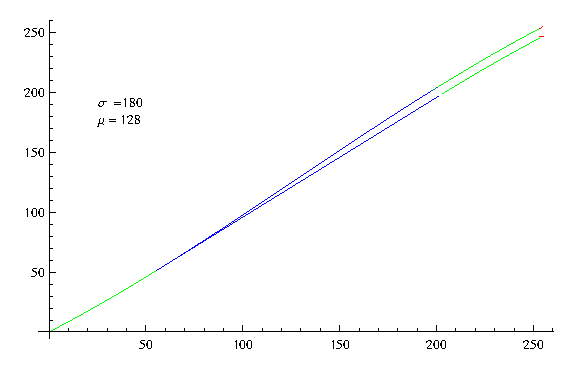
\includegraphics[width=0.49\textwidth]{Chapter2/Figs/linearSmooth2.eps}
    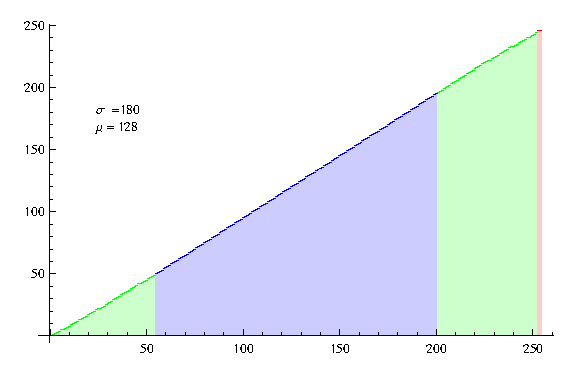
\includegraphics[width=0.49\textwidth]{Chapter2/Figs/linearColor2.eps}
    \caption{Linear approximation.}  \label{fig:Linear}
\end{figure}

\begin{figure}[h!]
  \centering
    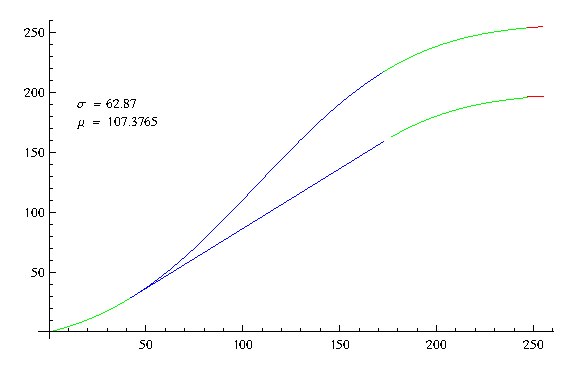
\includegraphics[width=0.49\textwidth]{Chapter2/Figs/ERFSmooth2.eps}
    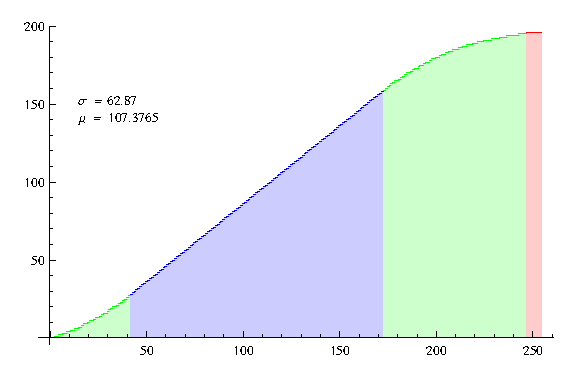
\includegraphics[width=0.49\textwidth]{Chapter2/Figs/ERFColor2.eps}
    \caption{Error Function distribution.}  \label{fig:ERF}
\end{figure}

There is one final value of interest to the development of the algorithm, which is the gradient at the mean. The reason this is of interest is because we're trying to compress the relevant data as much as possible. If the destination region is small (i.e. the destination machine type is smaller than the source type), then the gradient at the mean allows us to assess the fidelity required of the source type. If it weren't for the fact that the source is the result of a rotation transformation, then there would be little purpose in assessing this value. However, it is entirely possible that the lengthening of the axes resulting from the rotation is insignificant for the desired destination type; there's no point preserving information during the rotation which is then discarded by the redistribution. The gradient is given by

\begin{equation}\label{eq:gradient}
\begin{aligned}
\Delta(\mu,\sigma) &= \kappa  \delta(\mu,\sigma)  & \delta(\mu,\sigma)  &= \frac{ \sqrt{2} }{ \sigma \sqrt{\pi }  \left(\Sigma^+-\Sigma^-\right)}
\end{aligned}
\end{equation}

The compression ratio is at most one-to-one, therefore $\kappa <=1$ and the gradient in the unit space must always be greater than 1 $ \kappa \le \Delta(\mu,\sigma) \le \delta(\mu,\sigma)$.

The required fidelity in the source domain can be found using $ \Delta$ in the sense that the correspondence between one information step in the source must produce a step of $\Delta$ in the destination type. For the algorithm evaluating the maximum gradient $\Delta$ allows us to be sure that  $\Lambda$ --- the region on the x axis where all the information is to be preserved --- exists if $\Delta >1$ or tells us that the x axis can be shortened if  $\Delta < 1$. In the algorithm $\Delta$ is used to find an appropreate working data type for the rotated color space and to define the axis scaling for the rotation matrix.

\section{The Skin Color Space Algorithm}

Now that all of the values necessary to preserve the skin information have been obtained, we can use them to build a color space transformation algorithm which can make intelligent decisions about the numerical precision for the intermediate and final variables, as well as determining the most efficient transformation methods. The algorithm described herein will take values of $\theta$, the rotation about the luminosity axis, the standard deviations and mean values for the two chromatic axes, and will automatically decide upon the necessary intermediate working data types and the most efficient redistribution methods.

During the color space conversion, the pixel values are represented in three different ways: input, working and output representations. At each stage, we are concerned with preserving the information from the previous stage required by the next. For this reason, we have defined terms for the mathematical analysis of the problem, as well as terms for the algorithm development. The terms associated with each stage are as follows:

\begin{tabular}{|c|c|c|c|}
  \hline
     Data Types & Src Pixel Values & Trans Pixel Values & Dst Pixel Values \\ \hline
  What? & Input & Working & Output \\ \hline
  Where? & Initial & After Rotation & After Re-Distribution \\ \hline
  Unit Range Value & $ \uSrc $ & $\uT$ & $\uDst$ \\ \cline{1-1}
  Int Range Value & $\iSrc$ & $\iT$ & $\iDst$ \\ \cline{1-1}
  Max & $\srcMax$ & $\tMax$ & $\dstMax$ \\ \cline{1-1}
  Min & $\srcMin$ & $\tMin$ & $\dstMin$ \\ \cline{1-1}
  Range & $\srcRange$ & $\tRange$ & $\dstRange$ \\
  \hline
\end{tabular}

Previously, we found the lengths of the new axes after the rotational transformation. If we were to keep the same data type for the color space as is used for the RGB values, then the axes would have to be rescaled with the accompanying loss of information. Given that we have values which allow us to assess where all the relevant information lies, a more sophisticated approach is possible. For a chromatic axis --- which, after rotation, has a length $L(\theta)$ --- we can determine the positions on that axis at which the information is considered irrelevant using Equation~(\ref{eq:LowHigh}) and the positions where the information is all considered relevant. If the gradient $ \Delta$ \ref{eq:gradient} is less than 1, then the distribution loses information at all points on the axis and the axis can be shortened without loss of relevant information. The only further consideration is to ensure that the values outside that range are prevented from causing errors associated with overflow. To exclude this possibility, a conditional statement can be used which checks the bounds as stated, assigning an appropriate value as necessary. The alternative is to use an intermediate value with a higher bit depth, and then to recast into the destination data type in such a way that overflow and underflow are handled appropriately. The OpenCV library provides a casting method --- "saturateCast" --- which serves this purpose.

We need to consider the requested compression of information alongside the spread of information caused by the rotation, and the desired focus on the specific region of interest dictated by the statistics. Each axis in the color space is to be represented by a discrete set of numbers. The size of these sets dictates the discretization of the axis, and the ratios between them indicates the spread or compression of the information they contain. We assume that the RGB axes are each discretized to the same extent, each containing $\srcRange$ values. After the application of the un-normalized rotational transformation, the axes contain differing numbers of values given by $\tRange_1 =\srcRange \; \sqrt{3} $, $\tRange_2 = \srcRange \; L_2(\theta) $  and $\tRange_3 = \srcRange \; L_3(\theta)$. These axis lengths preserve all the information contained in the source color space, and so are the maximum length the axis should take. The minumum length the axis may take is where the information is lost evenly throuought the axis, and corresponds to an axis length equal to the destination axis length $\tRange = \dstRange$. 

\begin{align}\label{eq:L2}
L_1 &= \sqrt{3} \\
L_2(\theta)  &= \sqrt{\frac{2}{3}} \sin \left(\widetilde{\vartheta}\right) + \sqrt{2} \cos \left(\widetilde{\vartheta}\right)  & where & & \widetilde{\theta} = \theta  \bmod \frac{\pi }{3} \\
L_3(\theta)  &= \sqrt{\frac{2}{3}} \sin \left(\widetilde{\theta}\right) + \sqrt{2} \cos \left(\widetilde{\theta}\right) & & & \widetilde{\vartheta} = \left(\theta - \frac{\pi }{6}\right) \bmod \frac{\pi }{3}
\end{align}

The destination color space is designed with a maximum discretization $\dstRange$ given by the required data type.

The analysis of the distribution is mathematically stated in a unit, source, and domain range. The maximum gradient of the distribution, when looked at in these terms, must always be greater than or equal to 1. This indicates a focusing of interest around the mean. It's not possible to extract more information than is contained in the source. For this reason, the destination axis may usefully only be shorter than or of equal length to the source axis. In terms of the machine representation, this indicates that the destination data type may be designed to contain a smaller range of values. The question for the rotational transformation is whether the rotated axis should be rescaled with the associated loss of information or not. We can now write an algorithm which determines the necessary scaling for the axes, and whether truncation of the extreme values is significant.

The length of the axis after rescaling should be

\begin{equation}\label{eq:RescaleAxis}
\min\left\{ \Delta(\mu,\sigma) , 1\right\} \srcRange \; \mathbf{L}(\theta)
\end{equation}

The condition for rescaling the axis is

\begin{equation}\label{eq:RescaleAxisCondition}
\Delta(\mu,\sigma) \le 1
\end{equation}

We can now re-formulate the transformation matrix in three different ways: pure rotation without rescaling, 

\begin{equation}\label{eq:Rotation}
 R_{xyz}(\theta) = \left(
\begin{array}{ccc}
 \frac{1}{\sqrt{3}} & \frac{1}{\sqrt{3}} & \frac{1}{\sqrt{3}} \\
 -\frac{\cos (\theta )}{\sqrt{6}}-\frac{\sin (\theta )}{\sqrt{2}} &
 \sqrt{\frac{2}{3}} \cos (\theta ) &
 \frac{\sin (\theta )}{\sqrt{2}}-\frac{\cos (\theta )}{\sqrt{6}} \\
 \frac{\sin (\theta )}{\sqrt{6}}-\frac{\cos (\theta )}{\sqrt{2}} &
 -\sqrt{\frac{2}{3}} \sin (\theta ) &
 \frac{\cos (\theta )}{\sqrt{2}}+\frac{\sin (\theta )}{\sqrt{6}} \\
\end{array}
\right) \quad \text{for} \quad  \Delta(\mu,\sigma) \ge 1
\end{equation}

maximum scaling --- which scales to the destination range


\begin{equation}\label{eq:NormRxyz2}
 \overline{R}_{xyz}(\theta) =
\kappa
\bigotimes
R_{xyz}(\theta) \quad where \quad
\begin{array}{c}
\kappa = \frac{\dstRange }{\srcRange \mathbf{L}(\theta)}
\end{array} \quad \text{for} \quad    \Delta(\mu,\sigma) \le \kappa
\end{equation}

 and scaled --- which shortens the axis as much as possible without losing statistically relavent data. 

\begin{equation}\label{eq:CompressedRotation}
 \widetilde{R}_{xyz}(\theta,\mathbf{\mu},\mathbf{\sigma}) =
\Delta(\mu,\sigma)
\bigotimes
R_{xyz}(\theta) \quad \text{for} \quad  \kappa < \Delta(\mu,\sigma) < 1
\end{equation}
because $\Delta$ is always greater or equal to $\kappa$ these special cases can be combined into a general scaling for each axis

\begin{equation}\label{eq:CombinedRotation}
 \widehat{R}_{xyz}(\theta,\mu,\sigma) =
\left(
\begin{array}{c}
\min\left\{\Delta(\mu_1,\sigma_1), 1 \right\} \\
\min\left\{\Delta(\mu_2,\sigma_2), 1 \right\}  \\
\min\left\{\Delta(\mu_3,\sigma_3), 1 \right\}  \\
\end{array}
\right)
\bigotimes
R_{xyz}(\theta) \quad where \quad
\begin{array}{c}
\kappa = \frac{\dstRange }{\srcRange \mathbf{L}(\theta)} \\
\Delta(\mu,\sigma) = \kappa \delta(\mu,\sigma)
\end{array}
\end{equation}
this produces a $\tRange$ of

\begin{equation}\label{eq:CombinedRotation}
\begin{aligned}
 \tRange(\theta,\mu,\sigma) &= \min\left\{\Delta(\mu,\sigma), 1 \right\} \srcRange \mathbf{L}(\theta) \\
 &= 
\left(
\begin{array}{c}
\min\left\{\dstRange \delta(\mu_1,\sigma_1), \srcRange \text{L}_1 \right\} \\
\min\left\{\dstRange \delta(\mu_2,\sigma_2), \srcRange \text{L}_2(\theta) \right\}  \\
\min\left\{\dstRange \delta(\mu_3,\sigma_3), \srcRange \text{L}_3(\theta) \right\}  \\
\end{array}
\right)
\end{aligned}
\end{equation}
\section{Setting up the 2-Channel Representation}\label{sec:SettingUp2-ChannelRepresentation}

For all computer vision tasks, the most significant influence on the required processing power is the number of channels. This is true even if the total information spread amongst the channels is less than the information contained in a single channel. Partly, this is due to the way that sequential processors operate; there is little difference between processing two 8-bit numbers and two 16-bit numbers on modern 64-bit processors. In contrast, processing a set of three related numbers is significantly more demanding; not only do the numbers have to be loaded into the processor sequentially, but the correlation between the numbers has to be taken into account. So, it is highly desirable to reduce the number of channels necessary for any further processing. The challenge is to compress all the relevant information for the desired subsequent processing into as few channels as possible.

It is not possible to compress all the information in such a way that it is appropriate for every computer vision application. It is, however, possible to tailor a compressing algorithm for a particular application.


\section{Skin Detection}\label{sec:SkinDetection}

With the image in the skin color space, skin detection is a significantly simplified problem; the average skin color is at the halfway point in both of the chromatic channels and the Gaussian distribution has already been applied, meaning that performing an elliptical thresholding in the normal color space is equivalent to a rectangular thresholding in the skin color space. The probability distribution can be obtained by combining the distributions in each chromatic channel. Because the thresholding levels in each channel are equivalent to the same points on the Gaussian, they can be straightforwardly combined, and then a single threshold used on the one resulting channel. This can be done by subtracting $\frac{1}{2}$ from both channels, squaring them, then adding them together.

The next step is to identify the skin. For the purposes of this project, we're searching for a skin-colored object of a specific shape: a finger that comes into the frame, presses down on a surface, then exits the frame. One of its properties is that it meets the edge of the frame, appearing as a rectangle with a rounded end which --- on occasion --- can appear slightly bent due to the viewing angle or pressure placed on the finger as it presses down on the surface. But there's a limit to how great that deflection can be in the image.

In order to find this shape, we begin by finding the contours in the binary probability image. This can be achieved by using the "findContours" method in OpenCV, which finds the contours and returns them as a vector of points. In the skin color space, finding the contours around the finger is very simple.

\begin{figure}[h!]
  \centering
      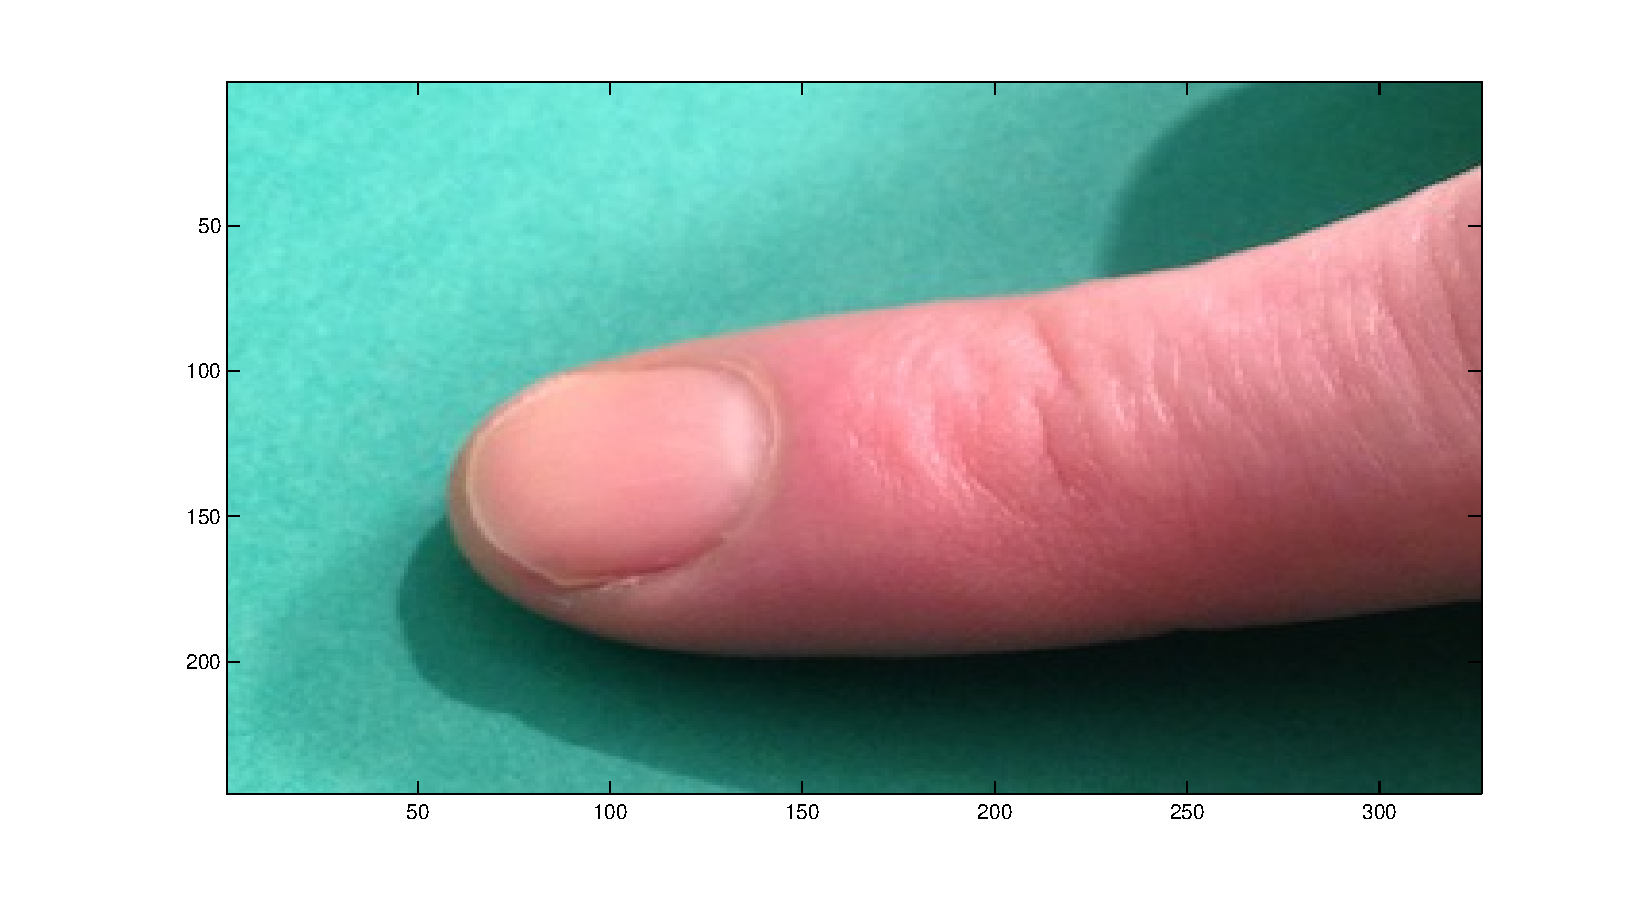
\includegraphics[width=0.45\textwidth]{Chapter2/Figs/imgJIndex1.eps}
    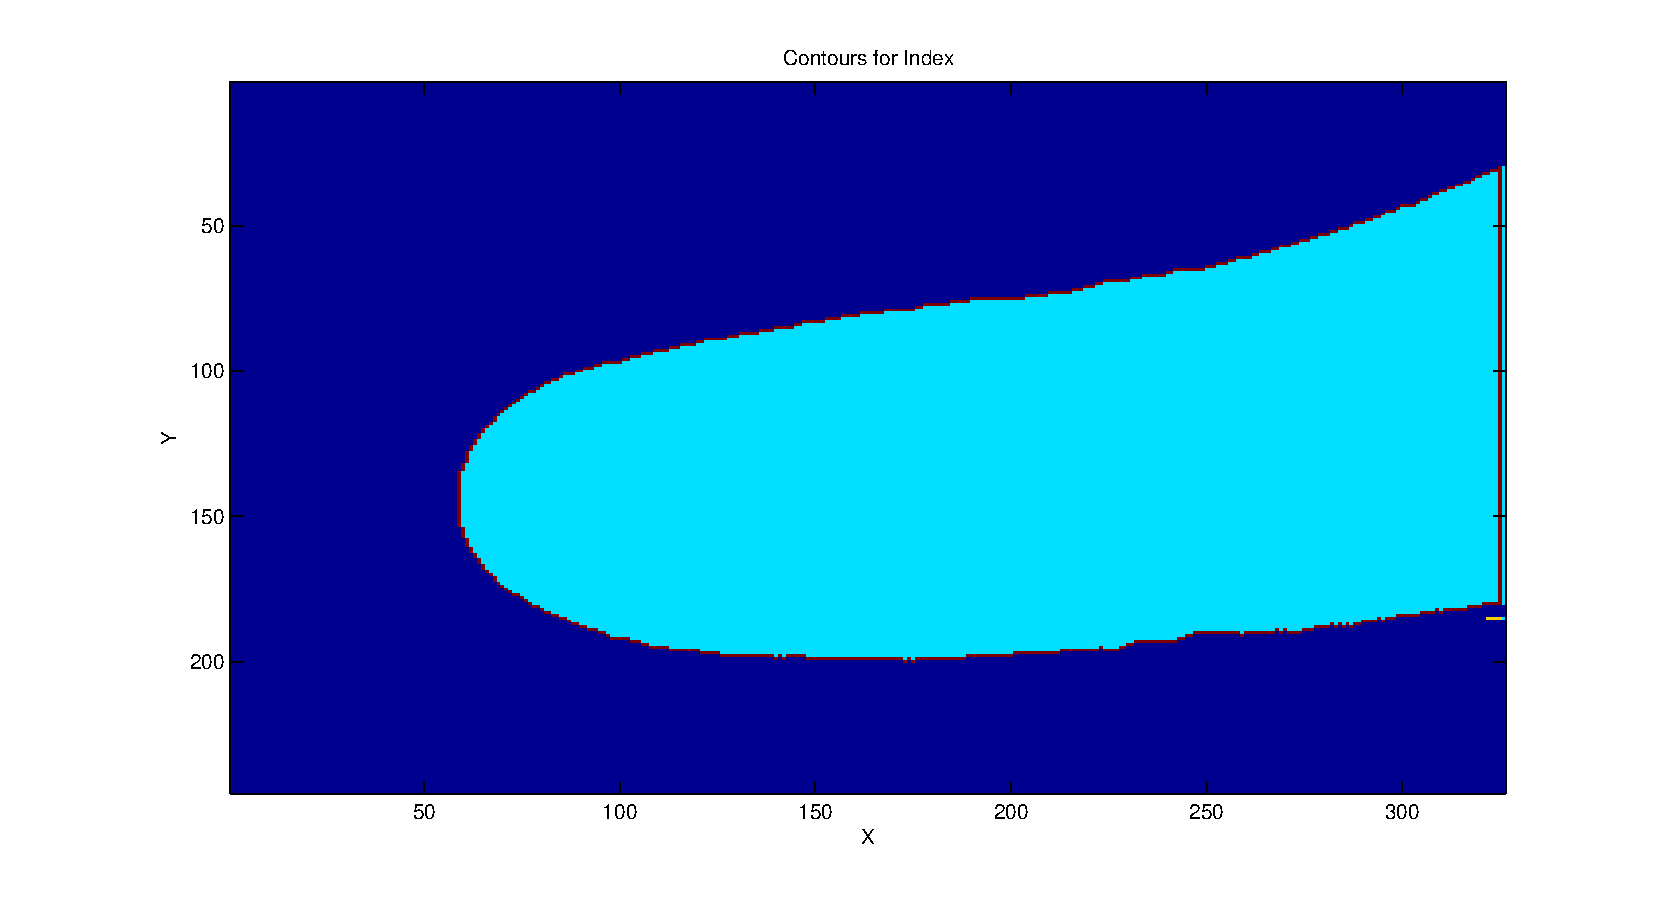
\includegraphics[width=0.45\textwidth]{Chapter2/Figs/indexContours.eps}
    \caption{Finger contours in the probability image.}\label{fig:IndexContours}
\end{figure}

Once the contours have been identified, a rectangle is drawn around the finger using OpenCV's "rectangle" method, with the tip of the finger touching one of its sides. Next, lines are drawn along the sides of the finger using the "line" method, and a convex hull identifies the semicircular fingertip, again using an OpenCV method, in this case "convexHull." This produces a set of verteces which allow us to locate the fingernail, at which point we highlight it with a square drawn using the "rectangle" method once more. The fingernail image within this square is then sent to the edge detector method for further processing. (See Figure 2.17.)

It should be noted that --- in the finger images in Figure~\ref{fig:IndexContours} --- the finger is deformed slightly due to the application of pressure on a flat surface, as was discussed previously. This doesn't necessarily share the same orientation as the tip. This can be remedied by taking the portion of the image highlighted by the rectangle and performing the operation again, thereby producing a rectangle which is properly oriented with the fingertip.

Once the fingertip has been identified, its features are obtained using the SURF algorithm method provided by OpenCV's SURF class. An initial attempt was made to use the library functions in OpenCV, however the high resolution and the relative uniformity of the fingertip resulted in no stable feature points being automatically detected. The initial idea was to allow the automatic descriptor generator to use a set of aligned frames and the idea was to keep the features which were stable in time and space. (i.e. Present in every frame and in the same location.) This attempt was unsuccessful, so a bespoke method was designed instead.

\begin{figure}[h!]
  \centering
    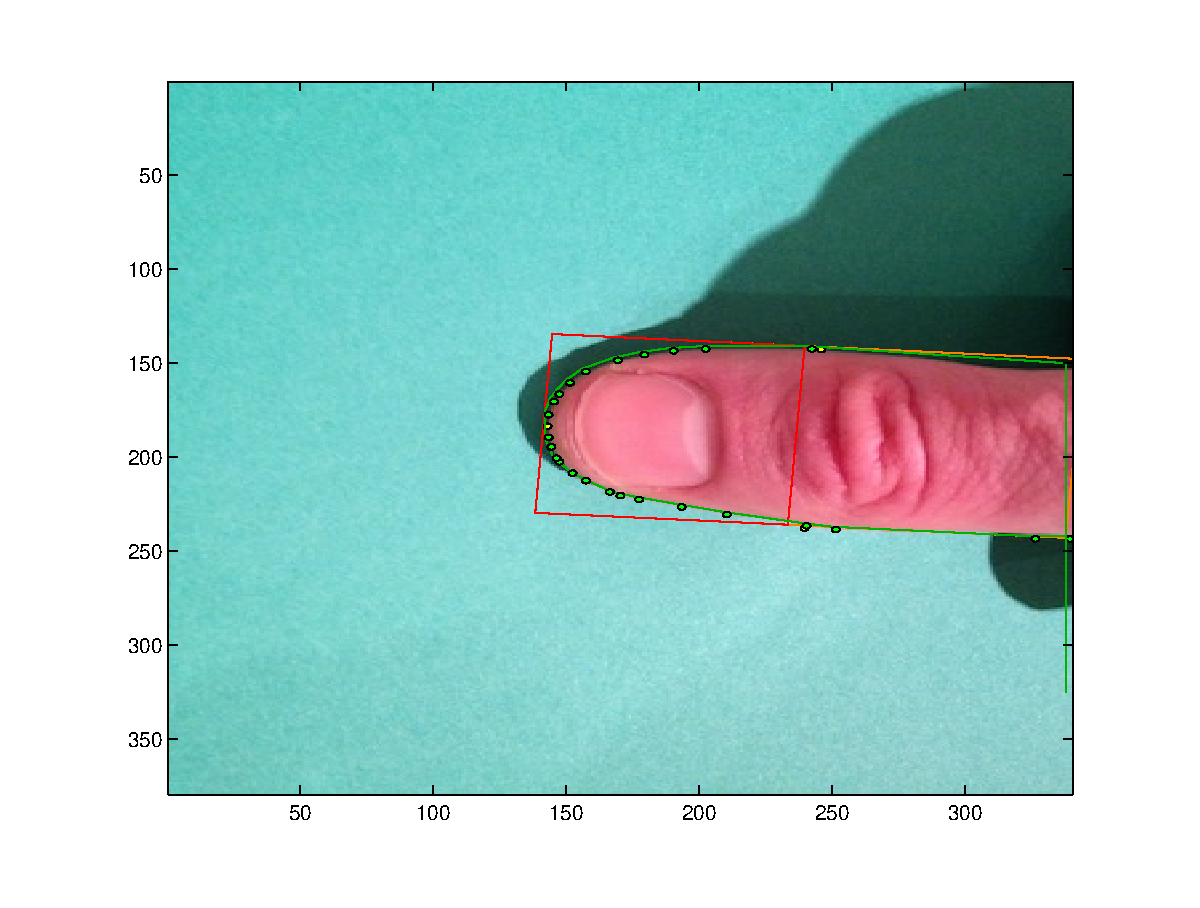
\includegraphics[width=\textwidth]{Chapter2/Figs/shapeDetection.eps}\label{fig:shapeDetection}
    \caption{Shape detection in action.}
\end{figure}

\begin{figure}[h!]
  \centering
    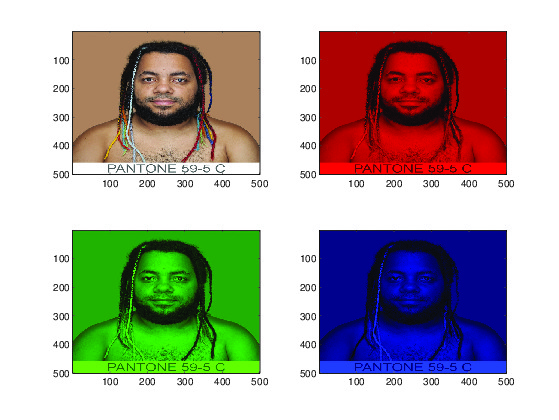
\includegraphics[width=\textwidth]{Chapter2/Figs/rainbowmanRGB.eps}
    \caption{RGB channels.}
\end{figure}

\begin{figure}[h!]
  \centering
    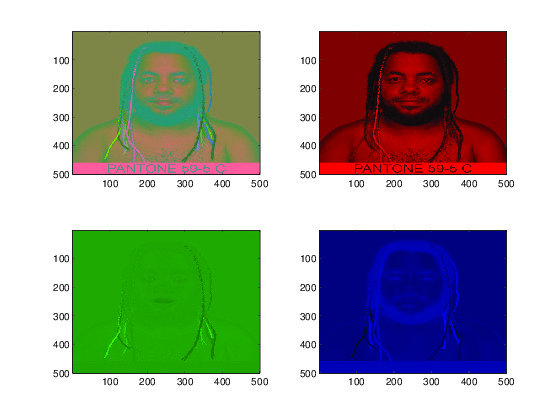
\includegraphics[width=\textwidth]{Chapter2/Figs/rainbowmanRotated.eps}
    \caption{Rotated color space.}
\end{figure}

\begin{figure}[h!]
  \centering
    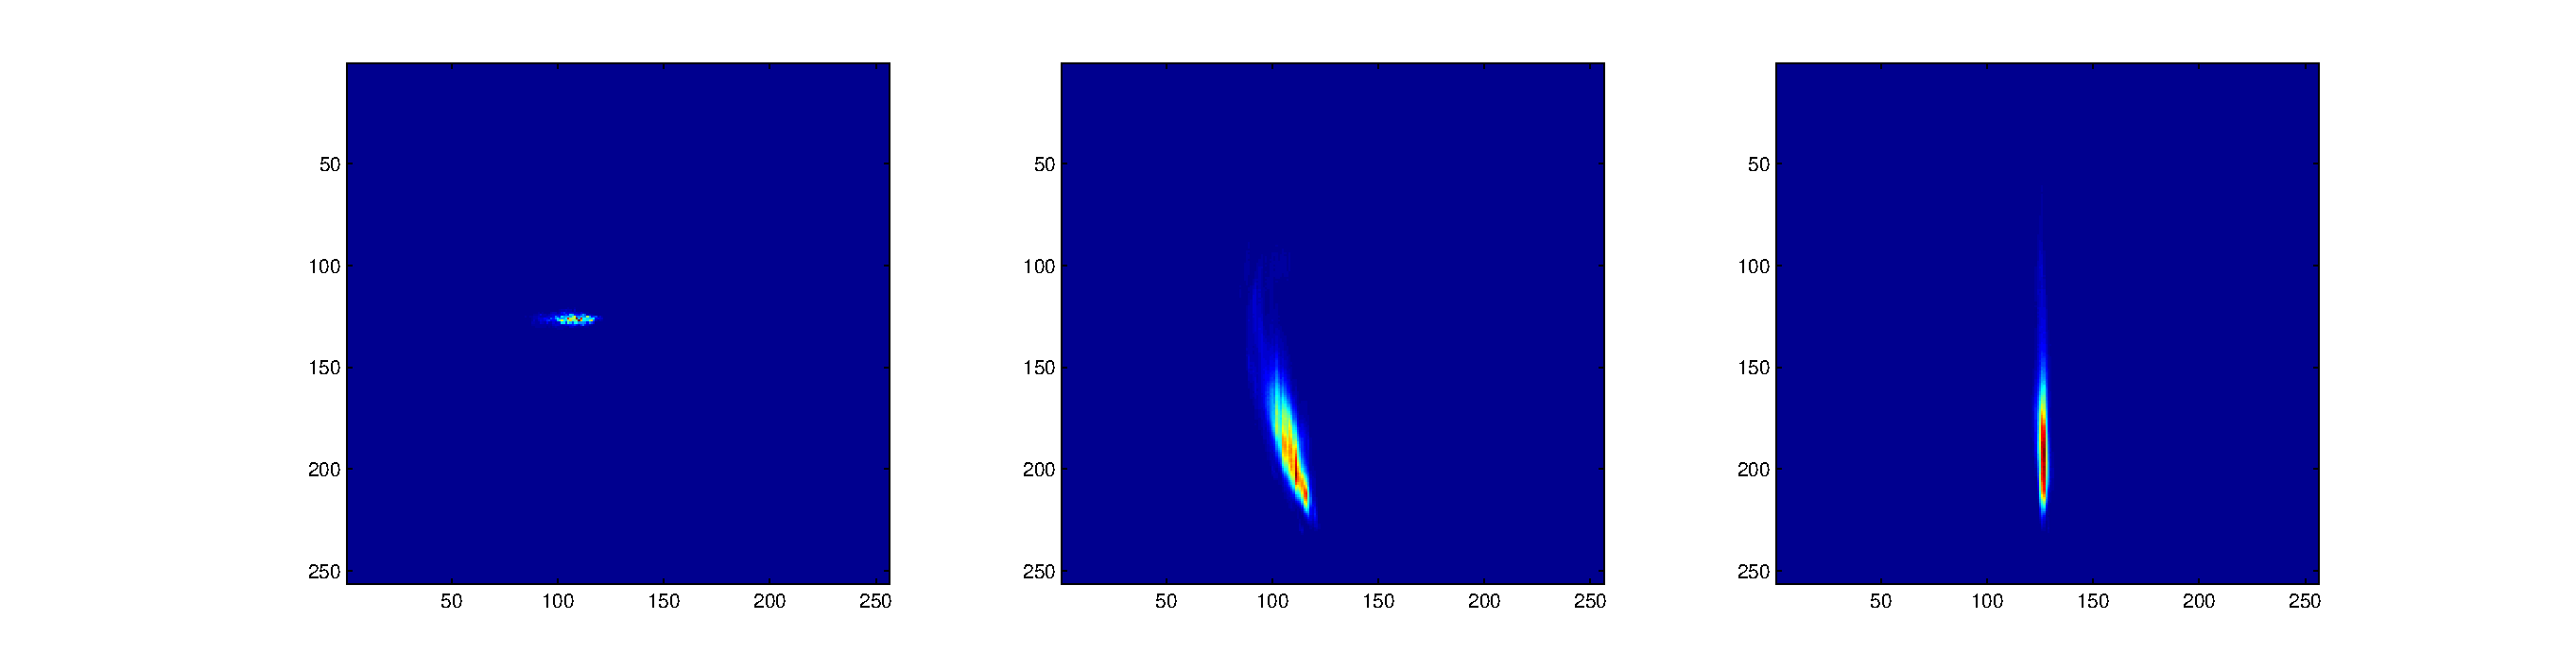
\includegraphics[width=\textwidth]{Chapter2/Figs/binsFinal2.eps}
    \caption{Final bins.}
\end{figure}

\begin{figure}[h!]
  \centering
    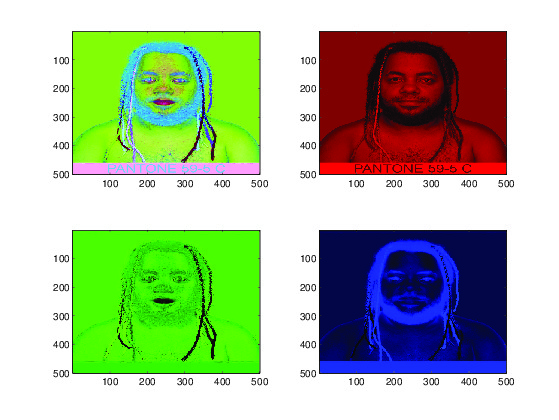
\includegraphics[width=\textwidth]{Chapter2/Figs/rainbowmanRotatedScaled.eps}
    \caption{Rotated and scaled color space.}
\end{figure}



%You know those blue/black people? Melanin may not be expressed in the fingernails!

%\subsection{Pigment vs. Blood}\label{sec:PigmentVs.Blood}

%\subsection{Blood Flow}\label{sec:BloodFlow}

%\subsection{Amplify the Effect}\label{sec:AmplifyTheEffect}


%\newcommand{\unitDst}{\text{uDst}} % Destination in the unit range 0:1
%\newcommand{\uDst}{\unitDst}       % Destination in the unit range 0:1
%\newcommand{\intDst}{\text{iDst}}  % Destination in the integer range dstMin:dstMax
%\newcommand{\iDst}{\intDst}        % Destination in the integer range dstMin:dstMax
%\newcommand{\dstMax}{\text{dstMax}}      % Destination integer range maximum
%\newcommand{\dstMin}{\text{dstMin}}      % Destination integer range mimimum
%\newcommand{\dstRange}{\text{dstRange}}  % Destination integer range
%\newcommand{\discreteDst}{\widetilde{\uDst}}   % Destination found using the discretized transformation matrix
%\newcommand{\dDst}{\discreteDst}               % Destination found using the discretized transformation matrix
%\newcommand{\delDst}{\delta\uDst}              % Error in the Destination found using the discretized transformation matrix
%
%\newcommand{\unitT}{\text{uT}}             % Rotated values in the unit range 0:1
%\newcommand{\uT}{\unitT}                   % Rotated values in the unit range 0:1
%\newcommand{\intT}{\text{iT}}              % Rotated values in the integer range tMin:tMax
%\newcommand{\iT}{\intT}                    % Rotated values in the integer range tMin:tMax
%\newcommand{\tMax}{\text{tMax}}            % Rotated values integer range maximum
%\newcommand{\tMin}{\text{tMin}}            % Rotated values integer range mimimum
%\newcommand{\tRange}{\text{tRange}}        % Rotated values integer range
%\newcommand{\discreteT}{\widetilde{\uT}}   % Rotated values found using the discretized transformation matrix
%\newcommand{\dT}{\discreteT}               % Rotated values found using the discretized transformation matrix
%\newcommand{\delT}{\delta\uT}              % Error in the Rotated values found using the discretized transformation matrix
%
%\newcommand{\unitSrc}{\text{uSrc}}       % Source in the unit range 0:1
%\newcommand{\uSrc}{\unitSrc}             % Source in the unit range 0:1
%\newcommand{\intSrc}{\text{iSrc}}        % Source in the integer range srcMin:srcMax
%\newcommand{\iSrc}{\intSrc}              % Source in the integer range srcMin:srcMax
%\newcommand{\srcMax}{\text{srcMax}}      % Source integer range maximum
%\newcommand{\srcMin}{\text{srcMin}}      % Source integer range mimimum
%\newcommand{\srcRange}{\text{srcRange}}  % Source integer range
%
%\newcommand{\unitX}{\text{uX}}       % Source in the unit range 0:1
%\newcommand{\uX}{\unitX}             % Source in the unit range 0:1
%\newcommand{\intX}{\text{iX}}        % Source in the integer range xMin:xMax
%\newcommand{\iX}{\intX}              % Source in the integer range xMin:xMax
%\newcommand{\xMax}{\text{xMax}}      % Source integer range maximum
%\newcommand{\xMin}{\text{xMin}}      % Source integer range mimimum
%\newcommand{\xRange}{\text{xRange}}  % Source integer range
%
%\newcommand{\unitY}{\text{uY}}       % Destination in the unit range 0:1
%\newcommand{\uY}{\unitY}             % Destination in the unit range 0:1
%\newcommand{\intY}{\text{iY}}        % Destination in the integer range yMin:yMax
%\newcommand{\iY}{\intY}              % Destination in the integer range yMin:yMax
%\newcommand{\yMax}{\text{yMax}}      % Destination integer range maximum
%\newcommand{\yMin}{\text{yMin}}      % Destination integer range mimimum
%\newcommand{\yRange}{\text{yRange}}  % Destination integer range
%
%\newcommand{\unitR}{\text{uR}}
%\newcommand{\uR}{\unitR}
%\newcommand{\intR}{\text{iR}}
%\newcommand{\iR}{\intR}
%\newcommand{\discreteR}{\widetilde{\uR}}
%\newcommand{\dR}{\discreteR}
%\newcommand{\delR}{\delta\uR}
%\newcommand{\rRange}{\text{rRange}}  % the discretization of the rotation matrix

\chapter{Skin Statistics}\label{sec:ChapSkin}
\epstopdfsetup{outdir=Chapter3/Figs/PDF/}
\ifpdf
    \graphicspath{{Chapter3/Figs/Raster/}{Chapter3/Figs/PDF/}{Chapter3/Figs/}}
\else
    \graphicspath{{Chapter3/Figs/Vector/}{Chapter3/Figs/}}
\fi

In order to identify the range of values for the skin space, a large number of skin samples were taken from photographs from the Humane project by Angelica Dass, an ongoing "chromatic inventory" art project which aims to compile every possible human skin color, categorized by the PANTONE guide color classification system~\cite{Dass2012}. The skin colors catalogued thus far are independent of race or ethnicity, so the samples are representative of human skin tones in general.

The image set consists of approximately 200 skin samples --- each of which shows only skin --- which are placed in a single directory in the file system. In accordance to our assumption that luminosity is not a significant factor in our skin model, we then perform the transformation initially with the value of $\theta$ equal to 0. The Matlab code collects frequency data for the rotated color space, incrementing the counts of a three-dimensional array of bins which span the color space. Viewing the frequency data along each of the three axes reveals that the skin image characteristics are spread widely in luminosity, but are quite confined in hue and saturation as illustrated in Figure~\ref{fig:InitBins}.


\begin{figure}[h!]
  \centering
    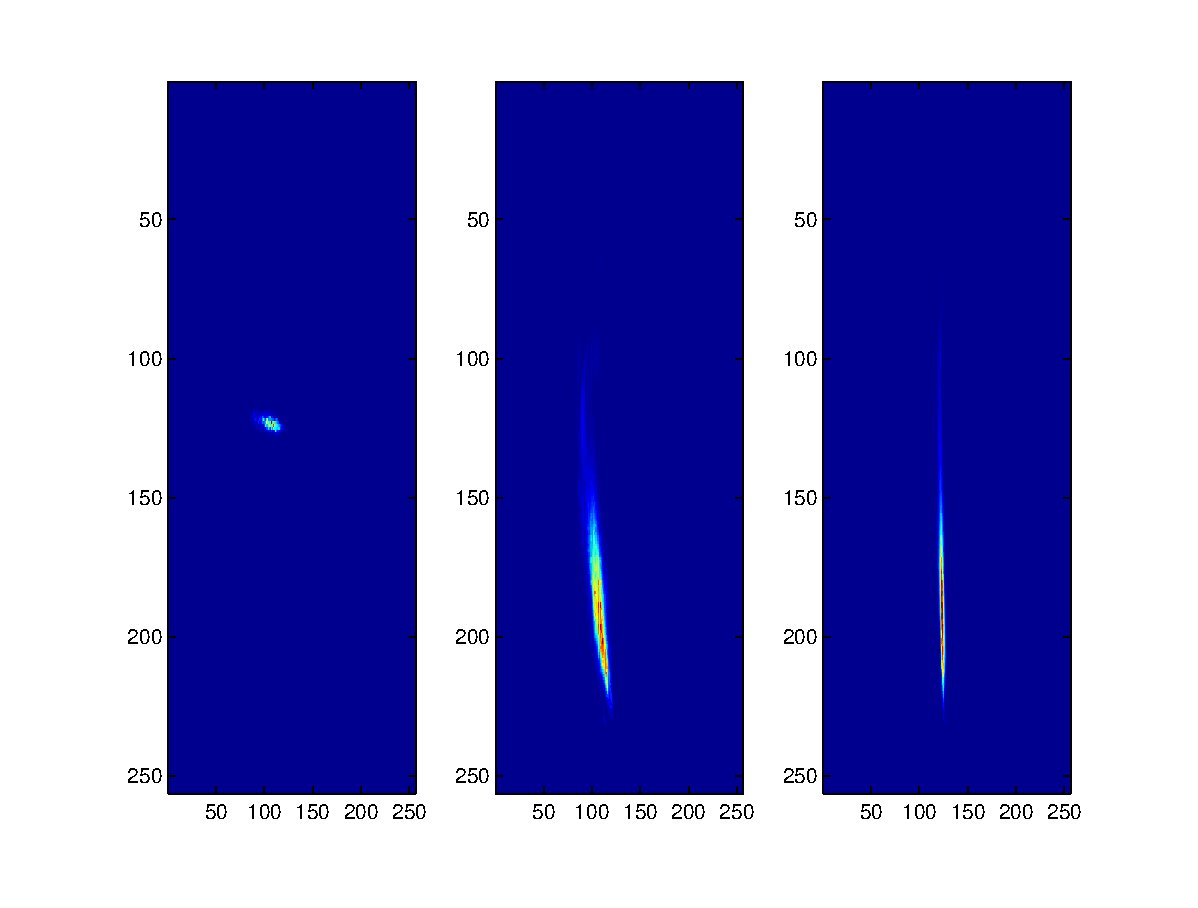
\includegraphics[width=\textwidth]{Chapter3/Figs/InitialBins.eps}
    \caption{Initial set of bins.}  \label{fig:InitBins}
\end{figure}


Aside from differing lighting, this is consistent with the notion that skin has a distinct pigmentation and justifies our attempt to find an appropriate color space disregarding luminosity. In doing so, the distribution of the skin color characteristics neatly fit into a 2-dimensional Gaussian distribution. The Matlab code produces a fit with a 2-dimensional Gaussian distribution and provides an angle relative to the orientation of the Gaussian fit to the skin sample distribution in the current color space.

Given that we are free to choose the orientation of the color space about the luminosity axis, the Matlab code allows us to find an orientation $\theta$ of the color space about the luminosity axis in which the distribution can be expressed as a product of 1-dimensional Gaussians along the axes. The final resulting distribution is presented in Figure~\ref{fig:DistributionAndGaussianFit}.


\begin{figure}[h!]
  \centering
    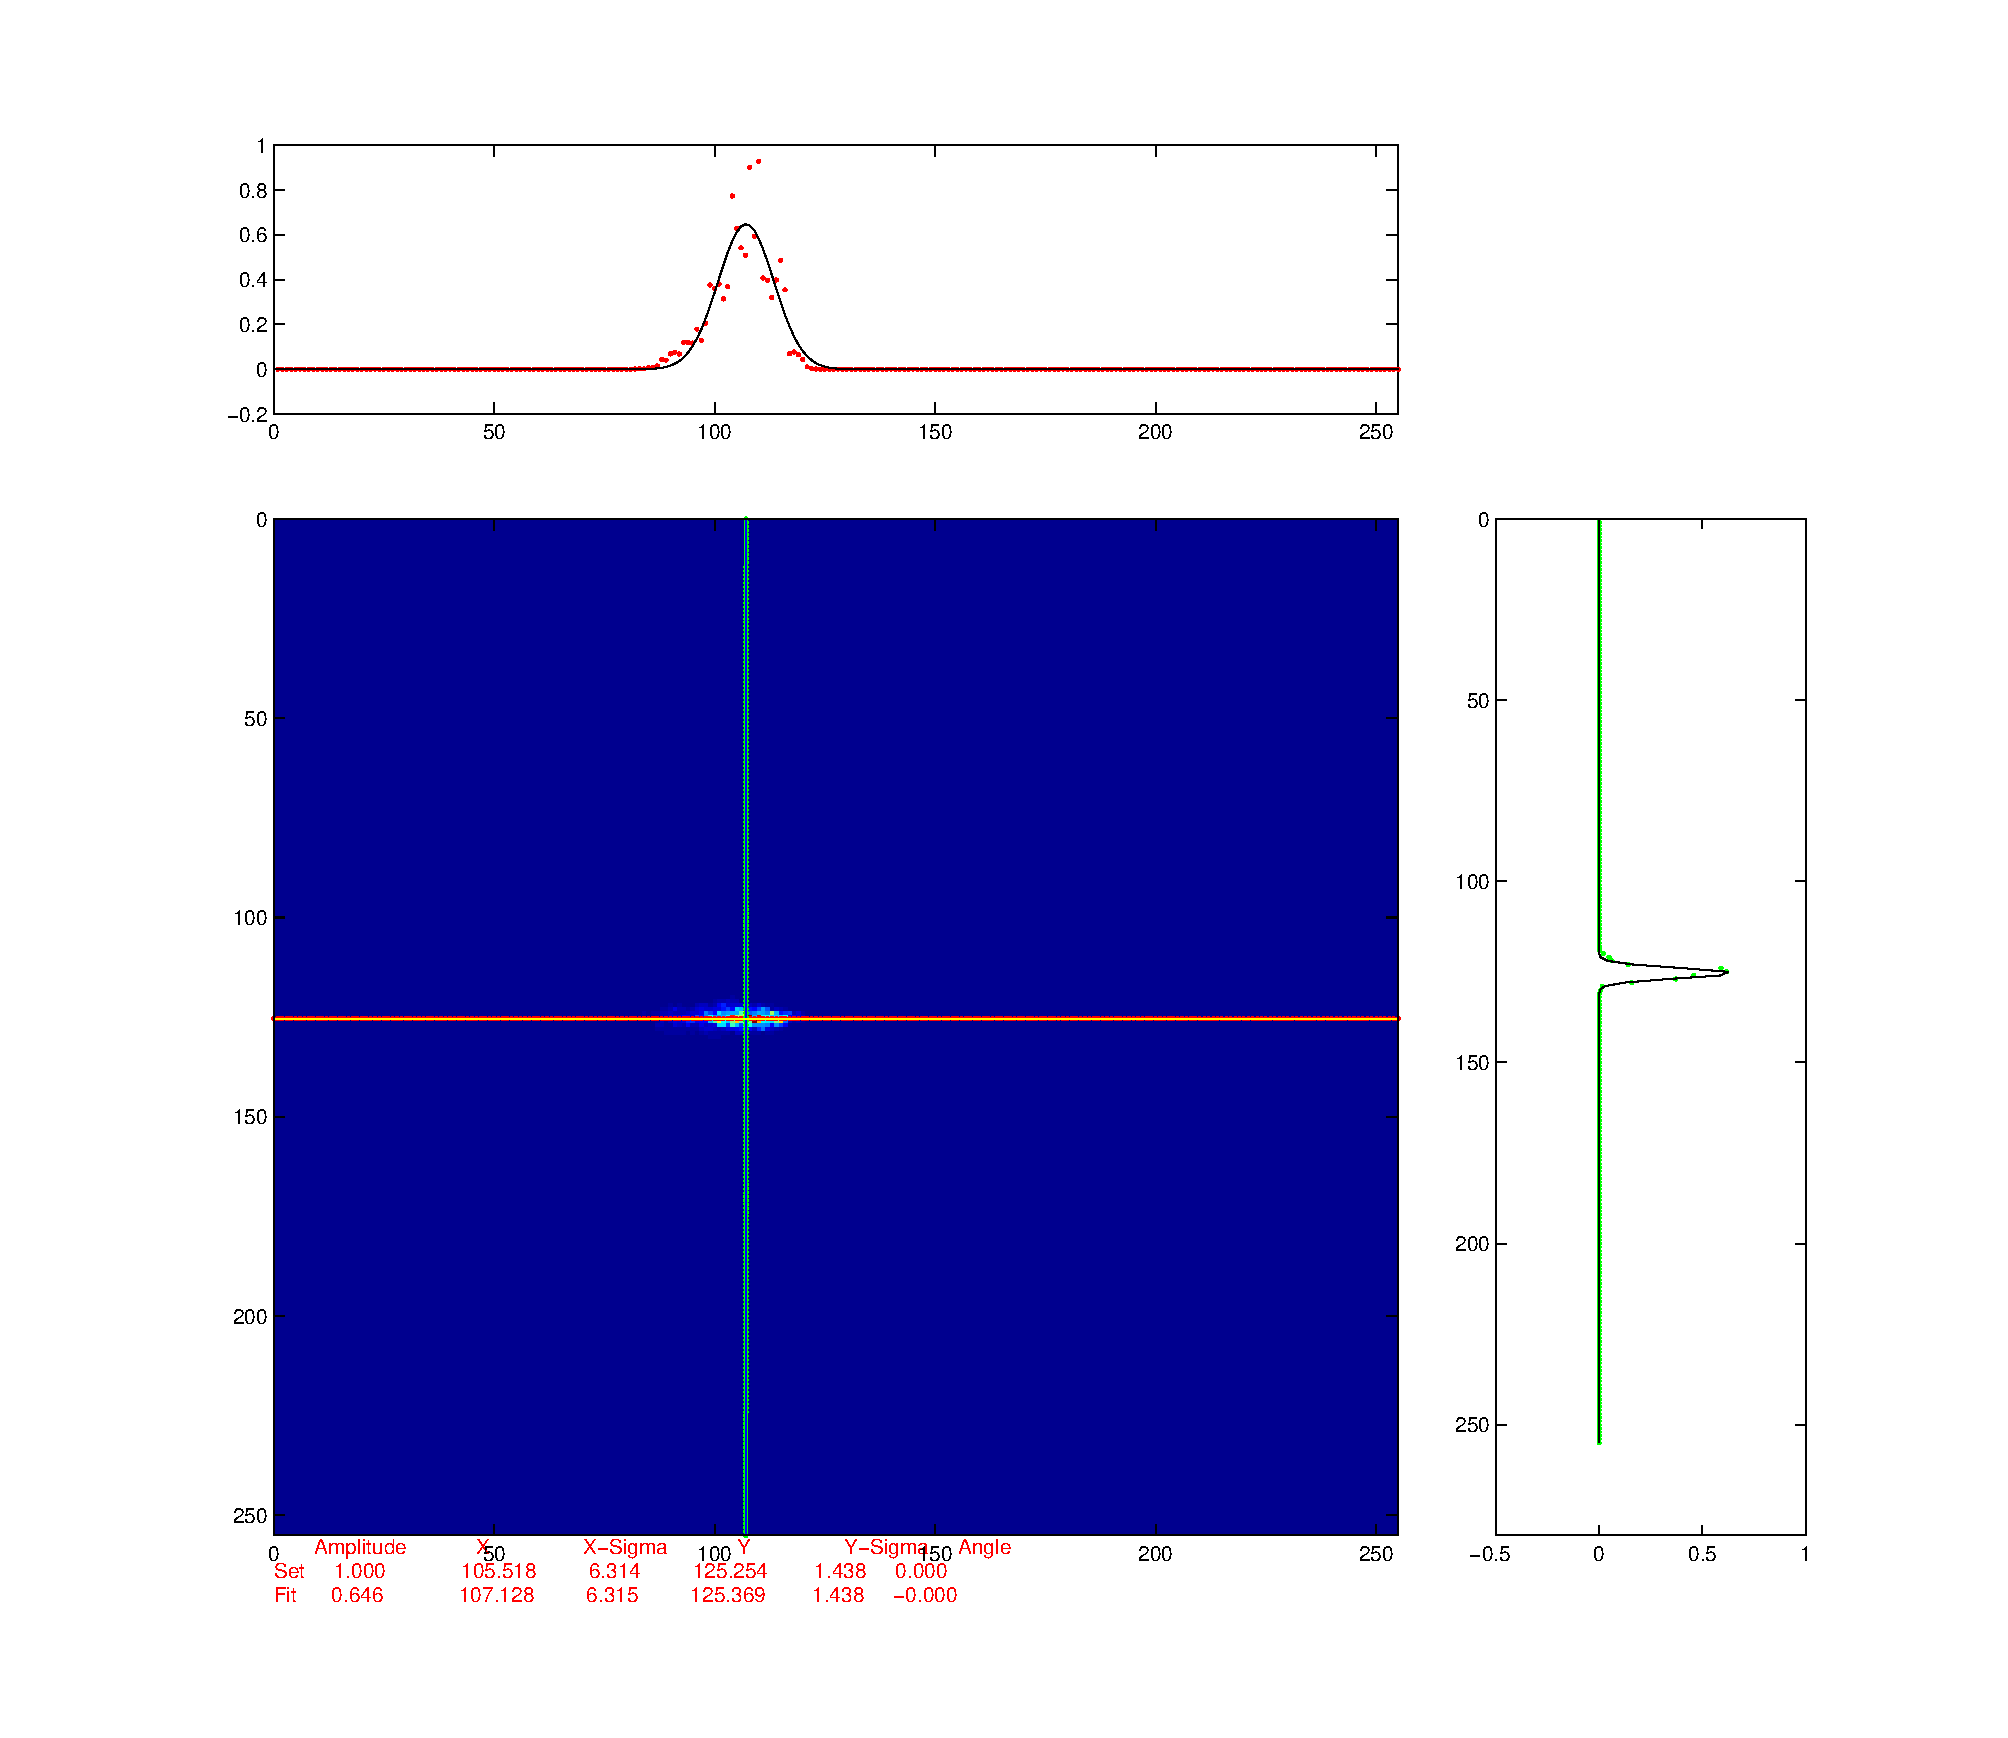
\includegraphics[width=\textwidth]{Chapter3/Figs/crosshairFigureFinal.eps}
    \caption{Distribution and Gaussian fit to the chromatic pixel values in the new color space.}  \label{fig:DistributionAndGaussianFit}
\end{figure}


For numerical reasons, the value for $\theta$ was found iteratively by performing the color space transformation and the statistical fit until the value for $\theta$ converged. (See Figure~\ref{fig:ConvergenceTheta}.)

\section{iPhone Camera Characteristics} \label{sec:iPhoneCameraCharacteristics}

Unlike more general cameras, the iPhone's camera performs certain pre-processing tasks on the raw image before it reaches the AP layer. Typically, cameras have a specific white point value, which is the value corresponding to white. It isn't necessarily the corner of the RGB cube; finding this value is part of the camera calibration. It also determines the orientation of the luminosity axis, which passes through zero to the white point. This is why all pre-defined color space functions have an implicit white point correction. However, the iPhone's white point is always set to the corner of the RGB cube before the image reaches the AP layer. So, when developing an algorithm for the iPhone, white point correction is not necessary, while on other devices the algorithm may need to be adapted accordingly.

\begin{figure}[h!]
  \centering
    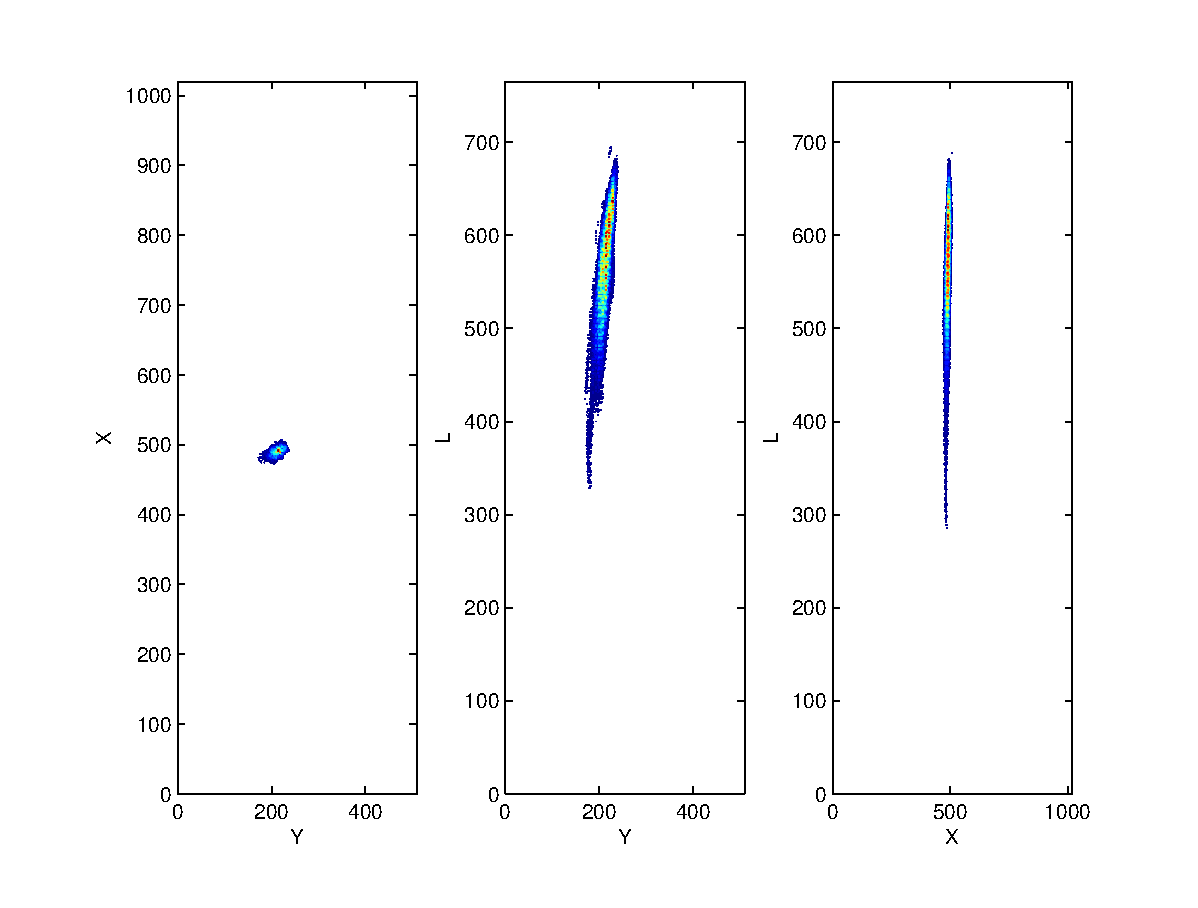
\includegraphics[width=0.80\textwidth]{Chapter3/Figs/lxy_general_white_point.eps}
    \caption{The white point for the general skin sample set described in Section~\ref{sec:SkinStatistics}.}  \label{fig:WhitePoint}
\end{figure}

While gathering skin statistics for the purposes of this project, the original approach involved taking photos of individual skin --- each with distinct color characteristics --- taken under different lighting conditions with a constant background using the iPhone camera. The background was included in order to obtain data on the edges of the skin. The background would be photographed, then again with each individual's hand over the same background. Afterward, the statistics would be collected and the background removed by negating the background statistics.

Surprisingly, this approached failed to work; the background reappeared (Figure~\ref{fig:BGFailure}).

\begin{figure}[h!]
  \centering
    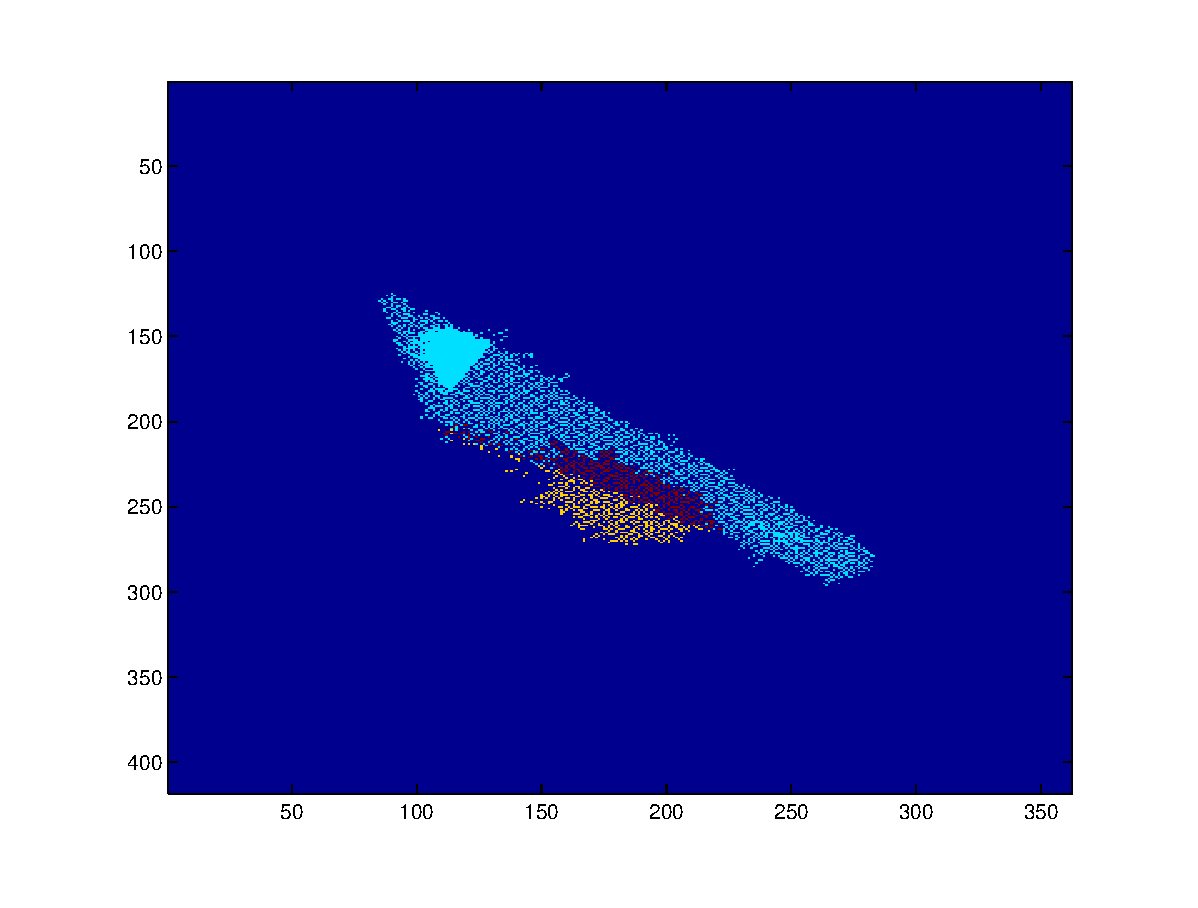
\includegraphics[width=0.60\textwidth]{Chapter3/Figs/xy_bg_failed.eps}
    \caption{Initial attempt at removing background; unsuccessful.} \label{fig:BGFailure}
\end{figure}

The background statistics changed with the skin present in the photo. This is because the iPhone adjusts to images with very strong color characteristics. This is an undocumented feature of the iPhone processing. The only way to compensate for this unwelcome pre-processing is to photograph the background with a strongly contrasting object present, but one which is easily cropped out of the image before the background stats are collected. After collecting the statistics again, the result was much improved (Figure~\ref{fig:BGSuccess}).

\begin{figure}[h!]
  \centering
    
\includegraphics[width=0.60\textwidth]{Chapter3/Figs/bg_cap.eps}
    \caption{The red marker cap contrasts with the green background.}  \label{fig:BGCap}
\end{figure}

\begin{figure}[h!]
  \centering
    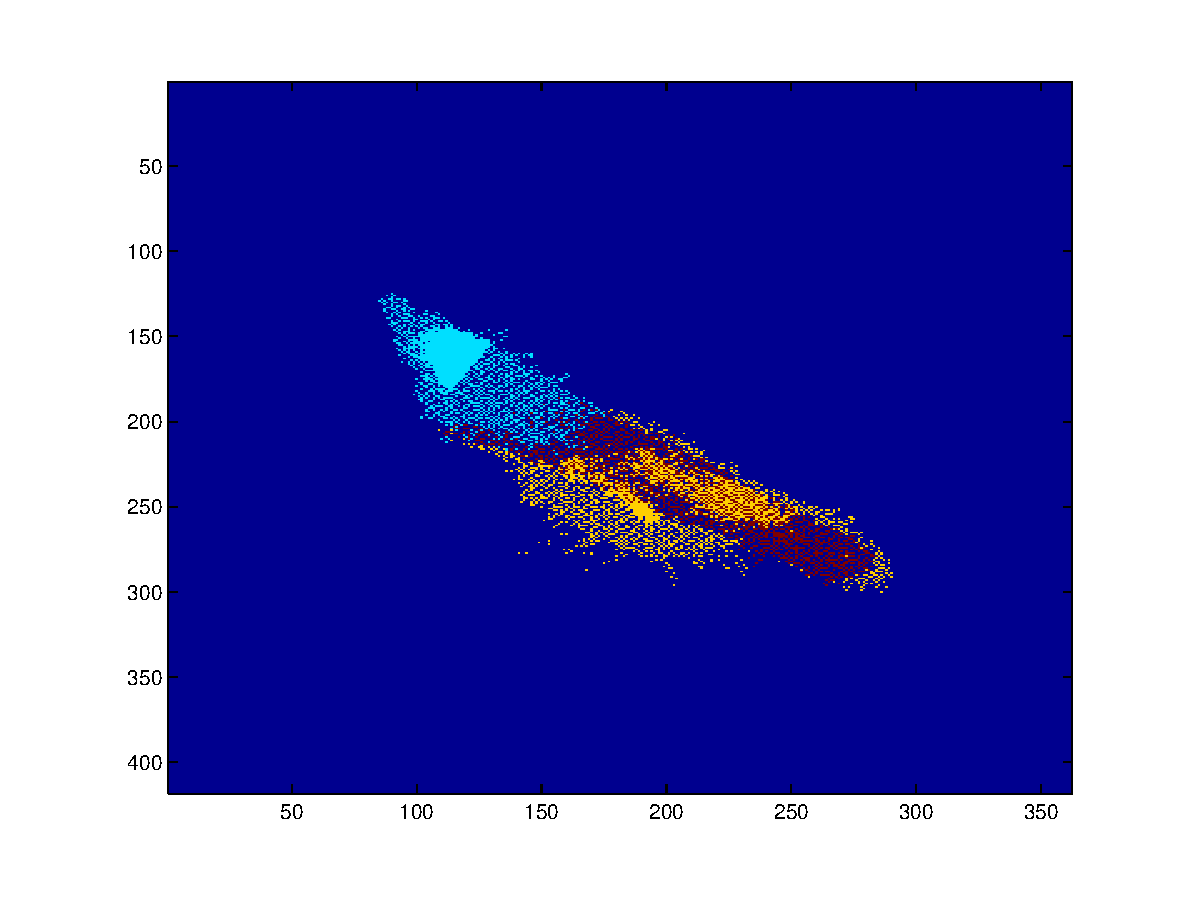
\includegraphics[width=0.60\textwidth]{Chapter3/Figs/xy_bg_success.eps}
    \caption{Successful background removal.}  \label{fig:BGSuccess}
\end{figure}

In a real world context, it is relatively safe to presume that the scene will be chromatically complex enough that the color correction won't be detrimental to detection, and perhaps even beneficial under unusual lighting conditions. But for gathering statistics, it proved to be a massive pain.


\section{Implementation of Skin Color Space Statistics in Matlab}\label{sec:SkinColorSpaceStatsMatlab}

A naive approach is to take a directory of images and process them using our color space transformation with the free angle $\theta$, processing them into three-dimensional pixel value bins. It was discovered that the region of interest is relatively small in this 3D space, so it was made possible the use of a bin of width greater than 1 lumio-chromatic value. However, it is quickly found that the region of interest is so small that using a more encompassing lumio-chromatic bin is actually detrimental to the numerics involved in finding and appropriate Gaussian fit, so a lumio-chromatic bin of width 1 is used.

Because the region is so small, when the transformation is applied, we must also retain all the information therein. Initially, we did not know this; our transformed images were represented as the same data type as the original. But because the transformed information is a less efficient representation of the original information, a significant amount of that information is lost.

\begin{figure}[h!]
  \centering
    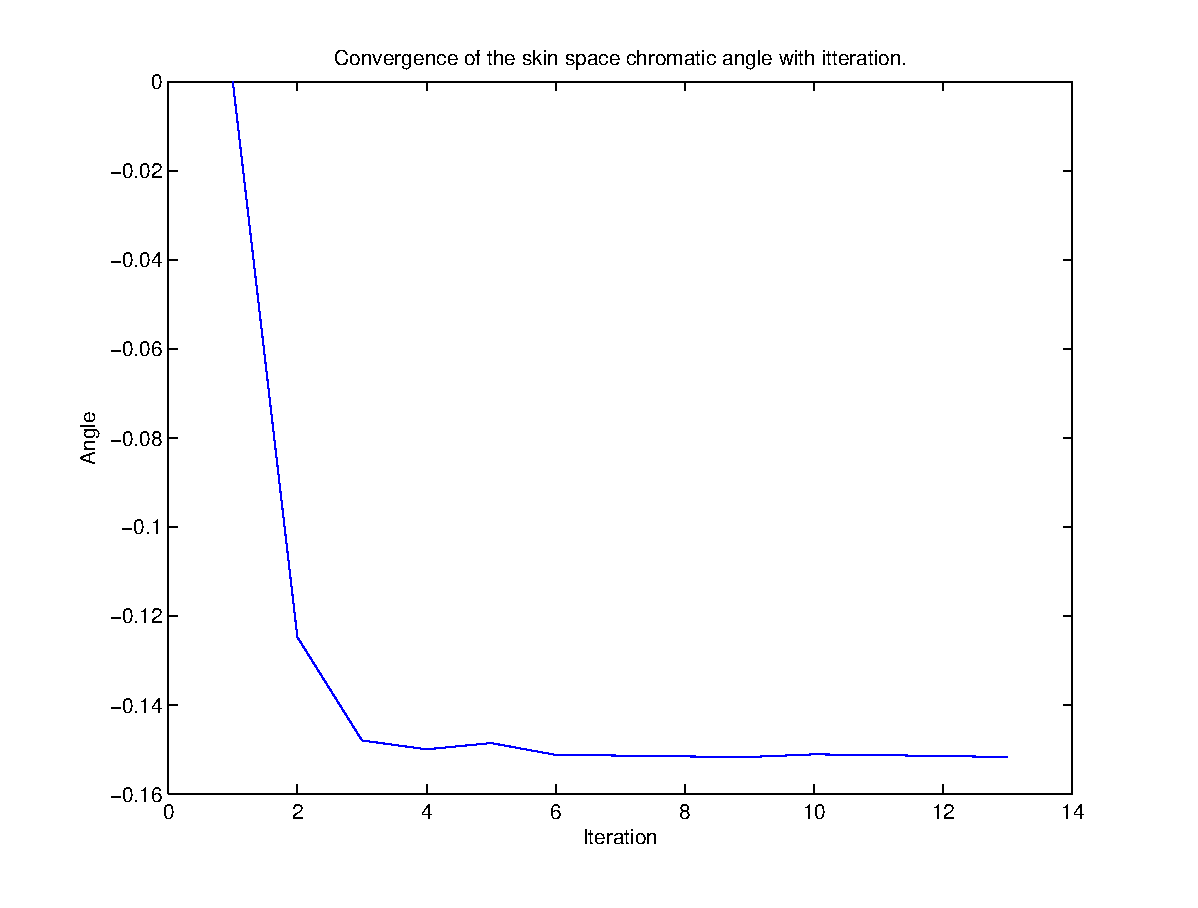
\includegraphics[width=\textwidth]{Chapter3/Figs/ConvergenceOfSkinSpaceFinal.eps}
    \caption{Convergence of color space orientation $\theta$.}  \label{fig:ConvergenceTheta}
\end{figure}

A better approach would be to iterate over the free angle $\theta$ of the Gaussian fit of the two-dimensional bin, which was found by collapsing the 3D bins along the luminosity axis, until convergence; at best, convergence was achieved after 3 iterations. Unfortunately, this approach --- though conceptually straightforward --- is very wasteful; all of the necessary information can be found in the RGB bin statistics.

Given that we are unable to apply this process in a reasonably efficient manner to individuals and general samples, if this project is to be finished sometime this century, a more nuanced approach is necessary.

\subsection{Transformation with Zero Angle}\label{sec:TransWithZeroAngle}

The more interpretable statistics for this project is a set of bins which contains all the information in the RGB bins, but is oriented such that there is a luminosity axis and two chromatic axes. Although the rotation matrices aren't unique, a set can be chosen and an angle $\theta$ determined in the chromatic space to be zero.

\begin{figure}[h!]
  \centering
    
\includegraphics[width=0.49\textwidth]{Chapter3/Figs/xy_Polygon.eps}
    \caption{The projection along the L axis showing the chromatic space with a free rotational angle of 0.}  \label{fig:xyPolygon}
\end{figure}



\subsection{Removing Zeroes}\label{sec:RemovingZeroes}

The obvious idea is to find all the non-zero bins and fit an interpolating function between them. This will effectively remove the empty bin artifacts within the densely-packed region which is the distribution we're interested in. However, the empty bins outside the main distribution are not artifacts and are genuinely empty bins, so removing all the empty bins and then fitting the function joins together any outlying points or secondary distributions corresponding to regions such as the background. We therefore desire a method which will allow us to keep all the non-empty bins and the empty bins outside the main distribution, i.e. all the genuinely empty bins. To achieve this, we designed a Matlab routine which essentially paints a region around each non-zero point, marking it as part of the main distribution. It then takes all the unmarked regions and includes all the empty bins in those regions. So, the set of points which is all the non-empty bins and all the empty bins in the unmarked regions satisfies the requirement, and a simple interpolating function can easily be fitted to those points.

%<flow chart, maybe? Or maybe at the end; we'll see.>

\subsection{White-Out and Black-Out}\label{sec:WhiteOutBlackOut}

Naively collapsing the bins along the luminosity axis artificially skews the chromatic distribution along the axis which passed through the luminosity axis; this is easily explained due to white-out and black-out. As luminosity increases or decreases, it will eventually hit the edge of the cube. Having reached its numerical limit, the luminosity slides toward the corner of the cube, resulting in a white or black value.

To accommodate this, we collapse the bins excluding the bins which are clearly suffering from white-out and black-out. This could be done mathematically by taking the bin of the distribution which is furthest from the luminosity axis, and then finding the intersection with the RGB cube when this chromatic value is at its limits, just before it reaches the edge of the cube where it suffers from white-out or black-out. But it's a simple matter to look at the three projections of the 3D LCaCb bins and manually determine the limits for the valid region.

%<Insert white-out/black-out bins here>

\subsection{Removing the Background Distribution}\label{sec:RemovingBGDistribution}

Having removed the empty bin artifacts and compensated for white-out/black-out effects, the final step is to remove the bin counts of the bins which are associated with the background, thereby leaving a distribution which corresponds to chromatic skin values and which is artifact- and systematic-error-free. With the chromatic bins processed as they have been so far, it is clear that there is a distinct distribution for the skin and a distinct distribution for the background. However, a distribution for the background was produced earlier, compensating for the iPhone's pre-AP-layer processing. Background removal is automated using a Matlab function which will negate the bins from one sample set using the distribution found for a second sample set.

%<Graph showing the overlap of the background and a skin background sample set; briefly describe what that shows.>

\subsection{Results}\label{sec:Results}

We're trying to develop a skin model from the Humane project, which provides a set which spans all the different skin tones. Although these images are not captured using the iPhone camera and thus suffer from a white point which does not correspond with the iPhone's white point (at least at the AP layer), it does provide a sufficient statistical basis to determine a color space region which is spanned by human skin. However, because of the iPhone camera's characteristics after pre-processing and the fact that the application needs to respond to an individual's skin, the investigation of skin tone characteristics for individuals is necessary.

To that effect, we selected three individuals with different skin tones; ordering by pigmentation from dark to light, we will henceforth refer to these as subjects F, N and J. Statistics were collected for the three subjects using the procedure outlined previously in this section. A two-dimensional Gaussian was fitted to the distribution for each individual.

\begin{figure}[h!]
  \centering
    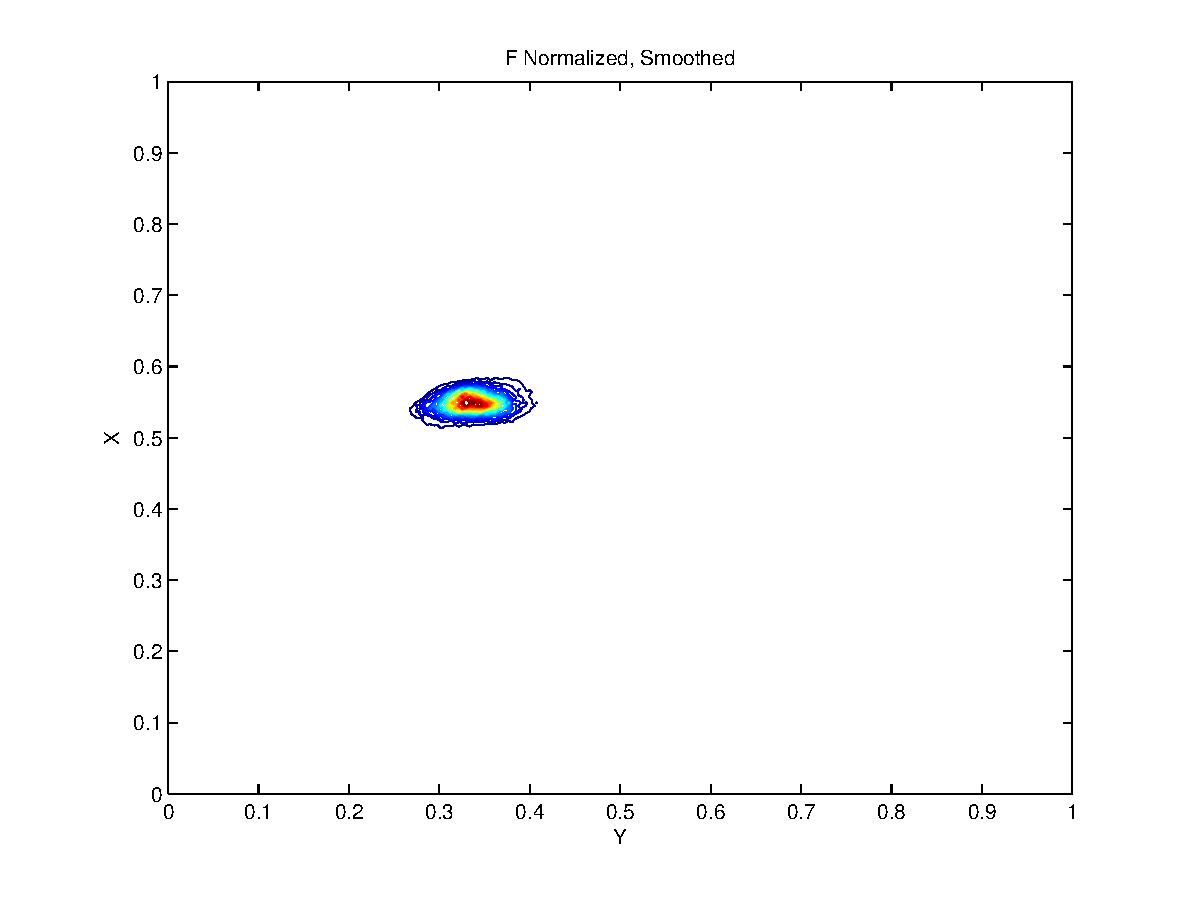
\includegraphics[width=0.49\textwidth]{Chapter3/Figs/FHands_XY_fBin.eps}
    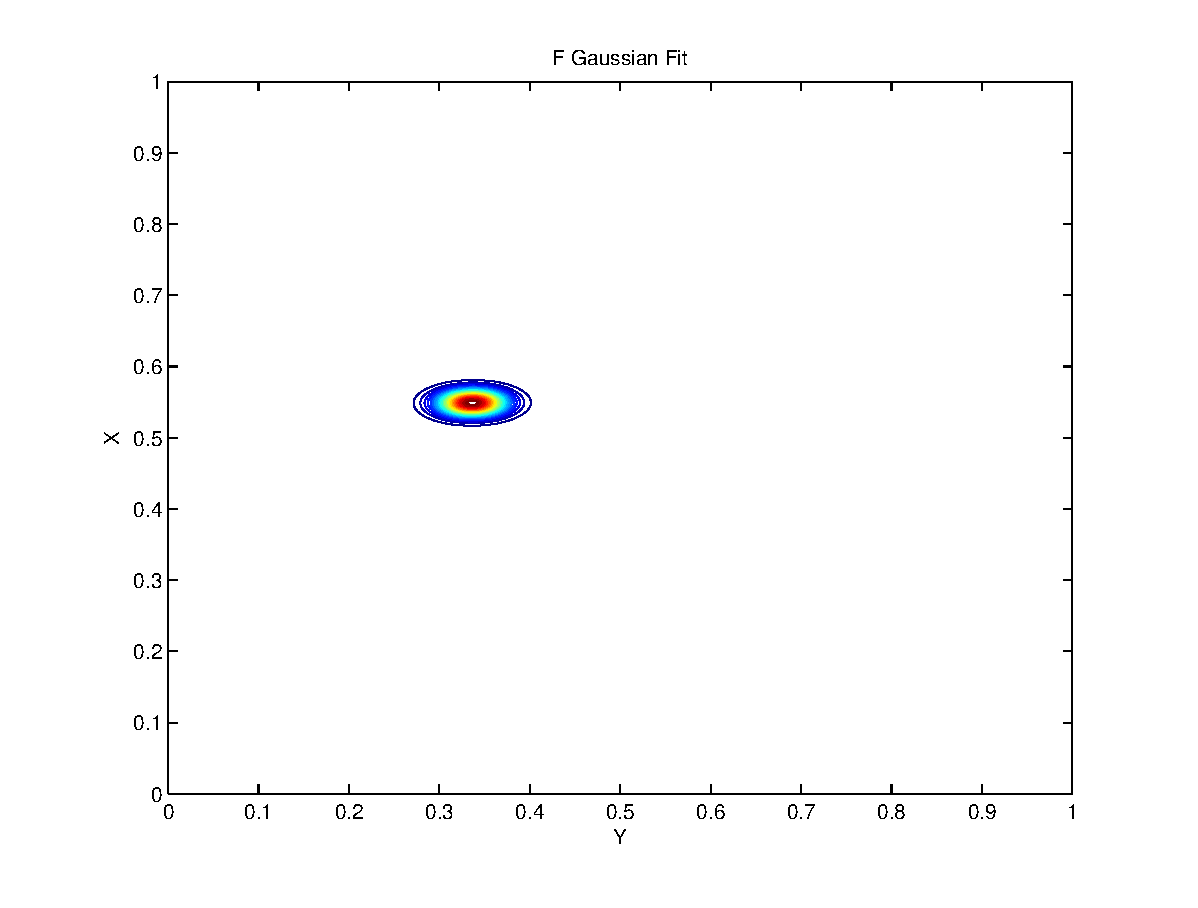
\includegraphics[width=0.49\textwidth]{Chapter3/Figs/FHands_XY_gFit.eps}
    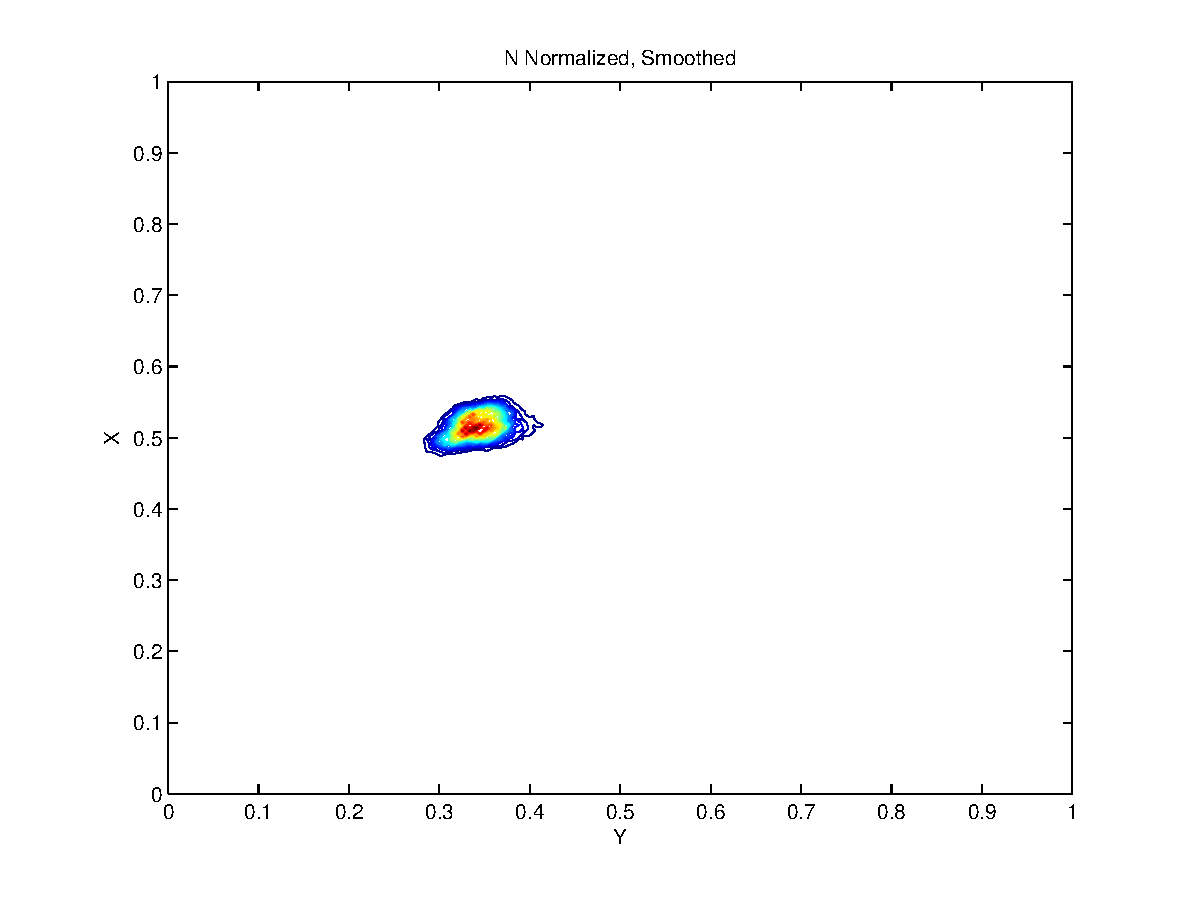
\includegraphics[width=0.49\textwidth]{Chapter3/Figs/NHands_XY_fBin.eps}
    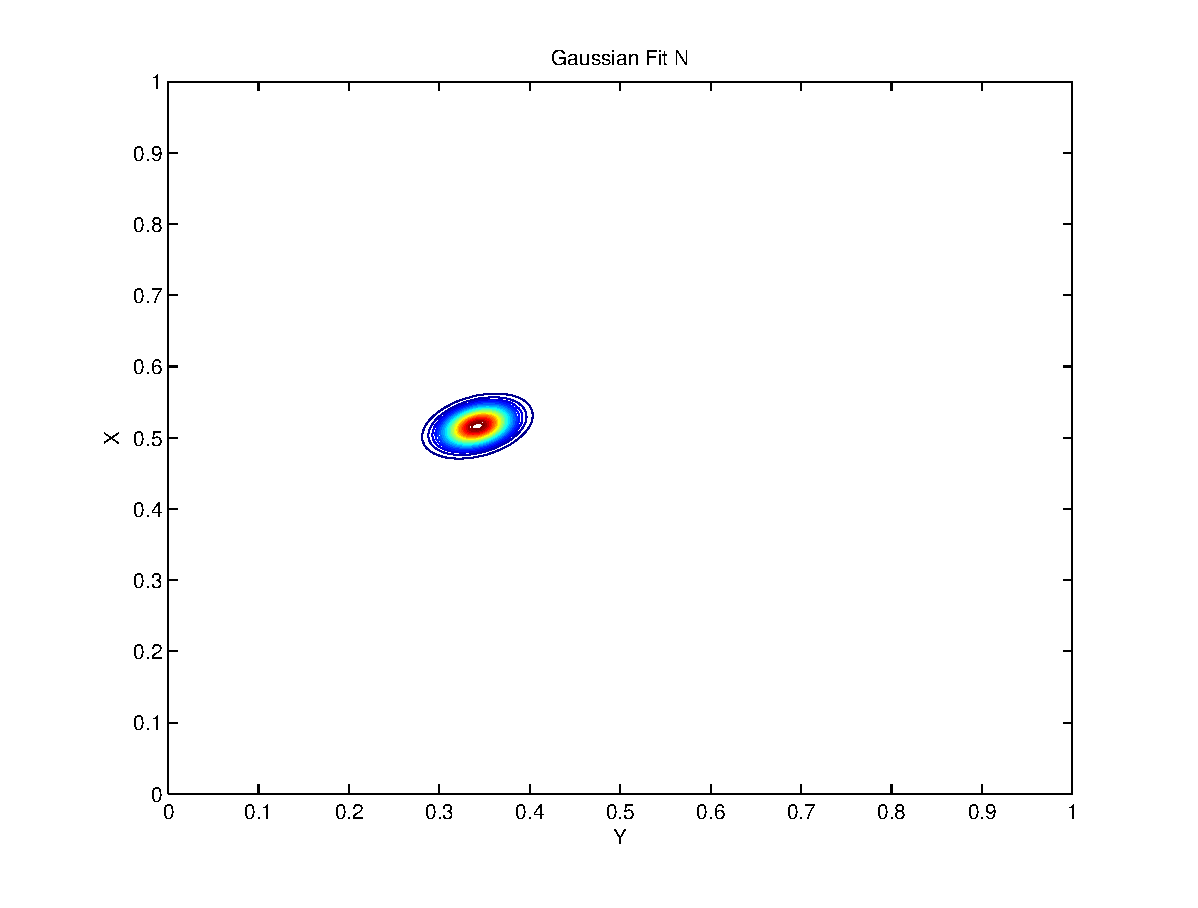
\includegraphics[width=0.49\textwidth]{Chapter3/Figs/NHands_XY_gFit.eps}
    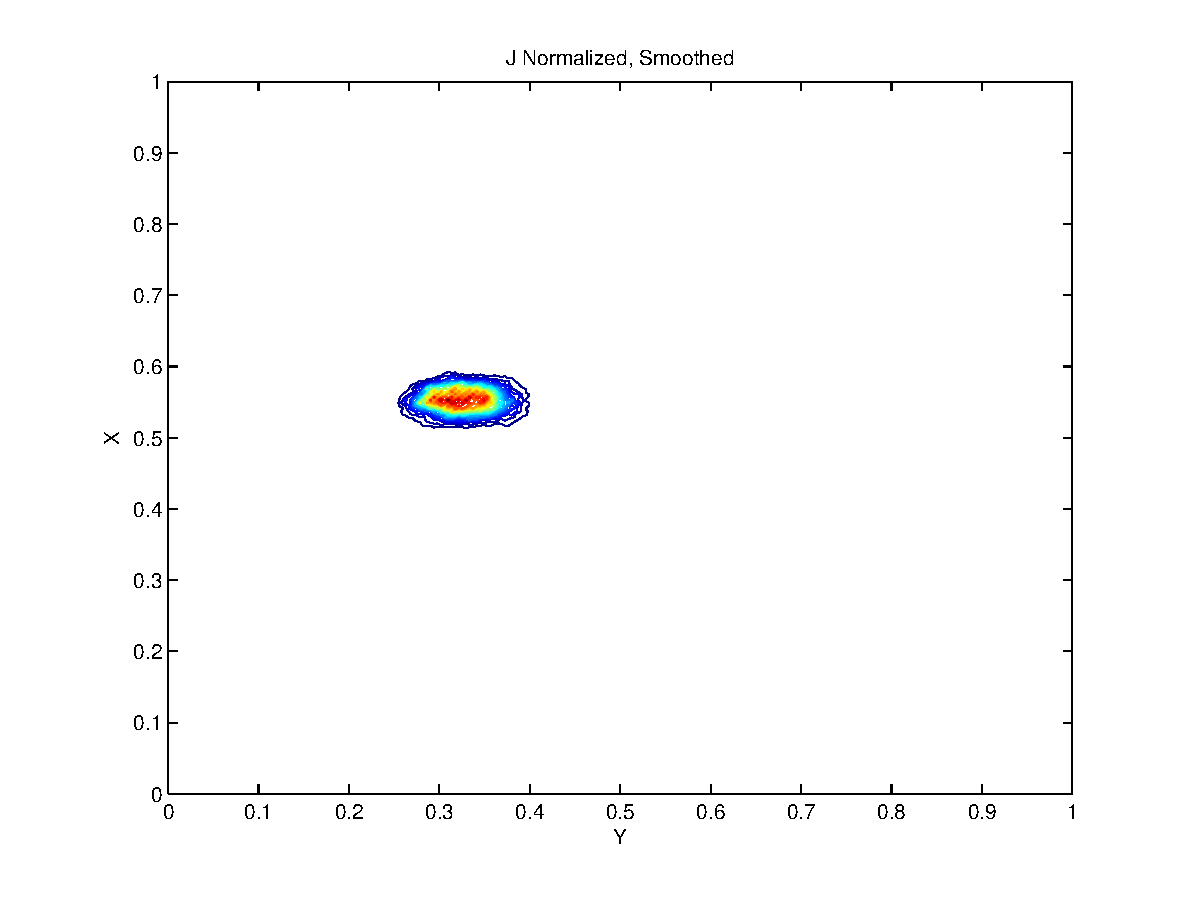
\includegraphics[width=0.49\textwidth]{Chapter3/Figs/JHands_XY_fBin.eps}
    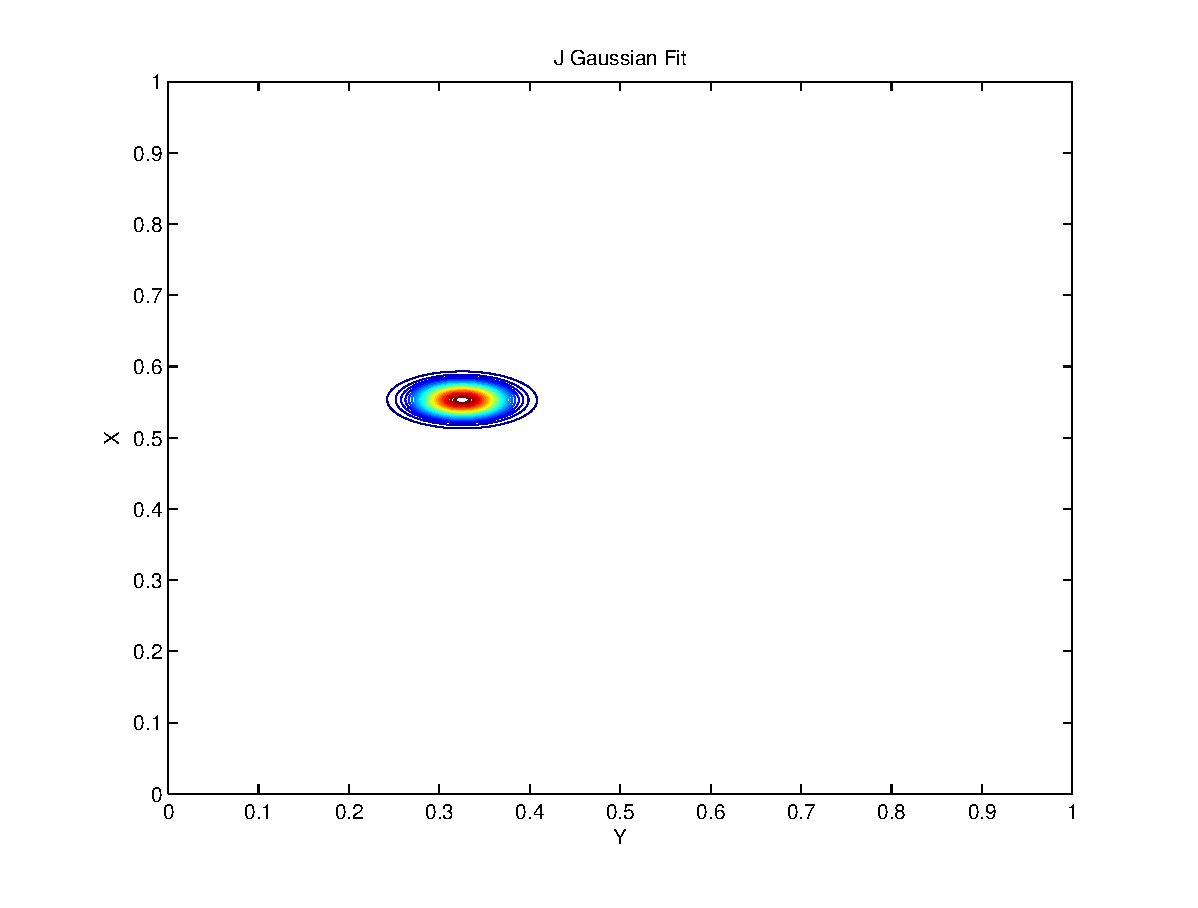
\includegraphics[width=0.49\textwidth]{Chapter3/Figs/JHands_XY_gFit.eps}
    \caption{The CaCb bins after processing and the Gaussian fit.}  \label{fig:FBinAndGFit}
\end{figure}

The individual statistics are as follows:
\newline

\begin{tabular}{|c|c|c|c|c|c|c|}
\hline
& \multicolumn{2}{|c|}{Mean ($\mu$)} & \multicolumn{2}{|c|}{Standard Deviation ($\sigma$)} & \multicolumn{2}{|c|}{Angle ($\theta$)} \\\hline
& X & Y & X & Y & Major Axis & Minor Axis \\\hline
F & 0.4249 & 0.3335 & 0.0081 & 0.0251 & -0.7724 & 0.7984 \\\hline
N & 0.4281 & 0.3443 & 0.0080 & 0.0195 & -0.5549 & 0.5969 \\\hline
J & 0.4022 & 0.3302 & 0.0119 & 0.0253 & -0.8954 & 0.6754 \\\hline
\end{tabular}
\newline
\vspace{0.5 cm}
\newline
The statistics for the general sample set are as follows:
\newline

\begin{tabular}{|c|c|c|c|c|c|c|}
\hline
& \multicolumn{2}{|c|}{Mean ($\mu$)} & \multicolumn{2}{|c|}{Standard Deviation ($\sigma$)} & \multicolumn{2}{|c|}{Angle ($\theta$)} \\\hline
& X & Y & X & Y & Major Axis & Minor Axis \\\hline
General & 0.4820 & 0.4253 & 0.0072 & 0.0108 & -0.1174 & 1.4534 \\\hline
\end{tabular}




\chapter{Pattern Recognition and Implementation}

% **************************** Define Graphics Path **************************

\epstopdfsetup{outdir=Chapter4/Figs/PDF/}
\ifpdf
    \graphicspath{{Chapter4/Figs/Raster/}{Chapter4/Figs/PDF/}{Chapter4/Figs/}}
\else
    \graphicspath{{Chapter4/Figs/Vector/}{Chapter4/Figs/}}
\fi


\section{Implementing the Color Space}\label{sec:ImplementingTheColorSpace}

In the previous two chapters, we have been approaching the color space design problem mathematically. Here, we will outline the practical implementation of the color space algorithm on the mobile device.

The first and most pressing consideration is limited processing power; while our mathematical approach to the algorithm design is significantly faster and more efficient than the more typical applications with commonly-used color spaces --- as will be discussed later in this chapter --- minimizing the number of clock cycles spent on continuous processes is necessary in order to ensure efficient operation. In the case of redistribution, the integer matrix transform is performed first, which puts the pixel values in the quantized working type qRsRange described in Chapter 2, then pixel classification is performed before any of the chromatic information is redistributed as illustrated in Figure \ref{fig:PartitioningRegions}.

The pixel classification is performed before the redistribution because it excludes processing pixels which are of no interest based on both chromatic channels, whereas for redistribution one channel may clearly lie outside of the discard region $\lambda$ while the other could be kept or redistributed. With the pixel classifier, if one channel lies outside the discard region, the other is also of no interest since the pixel value is outside of the partitioning region, thereby avoiding unnecessary processing time spent on redistribution. The classification is straightforward within the limits on the channel values, so it isn't sophisticated like an elliptical partitioning or a probabilistic Gaussian-based thresholding; it is simply a quick way of excluding the majority of the pixel values which aren't of interest.

Once the pixels have been classified, the redistribution is performed --- which requires further processing --- or we assign a pixel value from a small set of possibilities and skip onto the next pixel values. The redistribution function is applied to the working type tRange, while the comparison and classification is done in qRsRange. This is because the information in tRange is compressed to avoid wasting space, and as a consequence of this it does not occupy the full data type. qRsRange, on the other hand, being the natural range multiplied by the quantization matrix qR, does occupy the full data type. Since the operation is simply a comparison between numbers, it is of no advantage to compress the information so tightly. Additionally, since qRsRange is a signed range, one could look at the bit indicating the sign and immediately tell whether or not a given value will be discarded. Once scaled to tRange, the redistribution function is applied --- which has a source range of tRange and a range dRange of the destination type --- as outlined in <insert section in Chapter 2 here>.

It should be noted that the region between the extended keep region and $\lambda$ is not especially large; for even a $5\sigma$ result, it's only tens of values wide, let alone hundreds. As such, we use a lookup table for the redistribution in our actual implementation, thus further reducing the processing overhead. It should also be noted that C++ has a lookup table threshold set to approximately 64, which makes up a quarter of a region in our case. If the redistribution region is larger than that, the error function approximation from Chapter 2 is implemented. This is mainly for future-proofing the implementation, however; given the limited size of the region, we fully expect to use a lookup table for all practical cases.

As another future concession, the facility to add pixel-based functions to the color space transform, such as the skin probability function mentioned at the end of the previous chapter, is allowed. The color space transform is a threaded process, so there is no way of knowing that the last pixel value that was processed by any given thread was an adjacent pixels, as the parallelization is handled by OpenCV's universal threading library implementations. Pixel-based functions, however, are per-pixel processes, and they come out as separate resulting channels, so they can be added to the color space transform without causing any conflicts.



\subsection{The White-Out Black-Out Algorithm}\label{sec:WhiteOutBlackOutAlgorithm}
We need to find the point at which a chromatic value begins to suffer from white-out and black-out. This is done by taking the corresponding RGB value for the chromatic point and illuminating and deluminating the point by shifting the channel values by the same amount, noting when each channel value becomes fully saturated or desaturated. This is done in the unit space so the results can be scaled to any working range. The algorithm for finding the theoretical values is given in algorithm \ref{algo:TheWhiteoutBlackoutAlgorithm}. 

\begin{algorithm}[H]
 \begin{algorithmic}
  \Require{ $Ca$, $Cb$ The chromatic values}
  \State \phantom{Require}  { $iLCaCb$ the transform to LCaCb from RGB; }
  \State \phantom{Require}  {  $LCaCb$ the transform to RGB from LCaCb}
 \Ensure{  The luminosity at which black out $L_{BO}$  and white out $L_{WO}$ occur.}
 \State \phantom{Ensu} { \begin{tabular}{l}
 $Ca_{min}  \le Ca \le Ca_{max}$   \\ 
 $Cb_{min}  \le Cb \le Cb_{max}$  
 \end{tabular}  \parbox{0.65 \textwidth}{The chromatic range which could be suffering from white-out or black-out}}
 
   \State  $pnt^{RGB} \gets iLCaCb(0.5, Ca,Cb)$ \Comment{Put the point in RGB space }
   \State  $O \gets Order(pnt^{RGB}, \#1> \#2)$ \Comment{The order of the RGB channels from largest to smallest}
   \State  $\Delta WO_1 \gets 1 - pnt^{RGB}_{O(1)} $ \Comment{Iluminate to make the largest channel value saturated}
   \State  \phantom{Set} $pnt^{(RGB, WO, 1)}_{O(1)} \gets 1 $ \Comment{The point where a channel is saturated }
   \State  \phantom{Set} $pnt^{(RGB, WO, 1)}_{O(2)} \gets  pnt^{RGB} _{O(2)} + \Delta WO_1 $ 
   \State  \phantom{Set} $pnt^{(RGB, WO, 1)}_{O(3)} \gets  pnt^{RGB} _{O(3)} + \Delta WO_1 $ 
   \State  $\Delta WO_2 \gets 1 - pnt^{RGB}_{O(2)} $\Comment{Iluminate to make the second largest channel value saturated}
   \State  \phantom{Set}$pnt^{(RGB, WO, 2)}_{O(1)} \gets 1 $ \Comment{The point where two channels are saturated }
   \State  \phantom{Set}$pnt^{(RGB, WO, 2)}_{O(2)} \gets 1 $ 
   \State  \phantom{Set}$pnt^{(RGB, WO, 2)}_{O(3)} \gets  pnt^{RGB} _{O(3)} + \Delta WO_2 $ 
     
     
   \State  $\Delta BO_1 \gets  pnt^{RGB}_{O(3)} $ \Comment{Deluminate by the smallest channel value}
   \State  \phantom{Set}$pnt^{(RGB, BO, 1)}_{O(1)} \gets  pnt^{RGB} _{O(1)} - \Delta BO_1  $ \Comment{The point where a channel is desaturated }
   \State \phantom{Set} $pnt^{(RGB, BO, 1)}_{O(2)} \gets  pnt^{RGB} _{O(2)} - \Delta BO_1 $ 
   \State \phantom{Set} $pnt^{(RGB, BO, 1)}_{O(3)} \gets  0 $ 
   \State  $\Delta BO_2 \gets pnt^{RGB}_{O(2)} $ \Comment{Deluminate by the second smallest channel value}
   \State  \phantom{Set} $pnt^{(RGB, BO, 2)}_{O(1)} \gets pnt^{RGB} _{O(1)} - \Delta BO_2 $ \Comment{The point where two channels are desaturated }
   \State  \phantom{Set} $pnt^{(RGB, BO, 2)}_{O(2)} \gets 0 $ 
   \State  \phantom{Set} $pnt^{(RGB, BO, 2)}_{O(3)} \gets 0 $ 
     
   \State  $pnt^{(WO, i)}\gets LCaCb(pnt^{(WO, i)}) $ \Comment{The white-out points in LCaCb color space}
   \State  $pnt^{(BO, i)}\gets LCaCb(pnt^{(BO, i)}) $ \Comment{The black-out points in LCaCb color space}
   
   \State  $L_{WO} \gets pnt^{(WO, 1)}_1$ 
   \State  $L_{BO} \gets pnt^{(BO, 1)}_1$ 
   \State  $Ca_{min}  \gets Min(pnt^{(WO, 1)}_2, pnt^{(WO, 2)}_2, pnt^{(BO, 1)}_2, pnt^{(BO, 2)}_2 )$ 
   \State  $Ca_{max} \gets Max(pnt^{(WO, 1)}_2, pnt^{(WO, 2)}_2, pnt^{(BO, 1)}_2, pnt^{(BO, 2)}_2 )$ 
   \State  $Cb_{min}  \gets Min(pnt^{(WO, 1)}_3, pnt^{(WO, 2)}_3, pnt^{(BO, 1)}_3, pnt^{(BO, 2)}_3 )$ 
   \State  $Cb_{max} \gets Max(pnt^{(WO, 1)}_3, pnt^{(WO, 2)}_3, pnt^{(BO, 1)}_3, pnt^{(BO, 2)}_3 )$ 
     
  \State \textbf{Return} {$L_{WO} , L_{BO} , Ca_{min}, Ca_{max} , Cb_{min}, Cb_{max}$ }
 
  \end{algorithmic}
    \caption{The White-Out Black-Out Algorithm}
    \label{algo:TheWhiteoutBlackoutAlgorithm}
 \end{algorithm}
 
 The theoretical values are adjusted by 10\% to account for the auto brightness and contrast adjustment performed by the phone as described in Chapter 3, Section \ref{sec:WhiteoutAndBlackout}. We only wish to adjust the bounds away from the luminosity axis. One of the chromatic bounds will be the luminosity axis $Ca=\frac{1}{2}$ or  $Cb=\frac{1}{2}$, as this is the white or black point. Whether the bound is the upper or lower limit depends on the starting point, so we define a function which performs the adjustment appropriately.
 
 \begin{equation}
 slack(x) = \begin{cases}
 (1-a) x     & x < \frac{1}{2} \\
 (1+a) x     & x > \frac{1}{2} \\
 \frac{1}{2} & x = \frac{1}{2} 
 \end{cases} \quad \text{where} \quad a = 0.1
   \end{equation}
 We can now write the condition for whether a value could have suffered from white-out or black-out. 
  \begin{multline}\label{eq:InWoBoRegion}
 (( 0 \le L \le  slack(L_{BO}) ) \vee ( slack(L_{WO}) \le L \le 1) ) \wedge  \\
 slack(Ca_{min}) \le Ca \le  slack(Ca_{max}) \wedge  \\
 slack(Cb_{min}) \le Cb \le  slack(Cb_{max})
  \end{multline}
  
  \subsection{The Region Classification and Partitioning Function}\label{sec:TheRegionClassificationAndPartitioningFunction}
  It is desirable to classify a pixel value after rotation but before redistribution, using channel limits by how well the value fits the target and by how reliable the value is given lighting conditions. This can be done to a degree, but it is necessary to assume reasonably uniform lighting conditions. The pixel values are classified by chromatic value as either inside the target region or outside in both axes, dividing the chromatic plane into nine regions, as illustrated in Fig \ref{fig:PartitioningRegions}. A rudimentary partitioning is performed by assigning 8 constants to the values outside the region around the mean. The luminosity is always evaluated, because all that is required is a scaling from qRsRange to the destination range dRange. 
  
  \begin{figure}[h!]
    \centering
      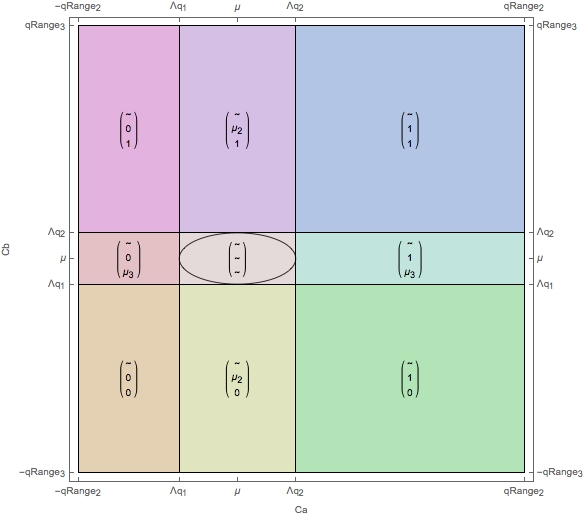
\includegraphics[width=0.80\textwidth]{Chapter4/Figs/PartitioningRegion.jpg}
      \caption{The Regions in the chromatic space. ~ Indicates values which will undergo redistribution. Regions outside the target area are allocated extreme values at the edge of the color space}  \label{fig:PartitioningRegions}
  \end{figure}
  
  
  
  \subsection{Floating the Mean}\label{sec:FloatingTheMean}
  Different lighting conditions can affect the detected pixel color. Not accounting for strongly-colored light, the affect of different lighting conditions is to increase or decrease the saturation of the color. The distribution is relatively unaffected in orientation or variance, meaning that lighting conditions can be accounted for by adjusting the mean. 
  \newcommand{\newMean}{\widetilde{\mu}}
  The algorithm adjusts to ambient lighting by first taking a reference image centered on a patch of skin and finding the mean in the LCaCb color space. This new mean $\newMean$ is then used in the current instance of the algorithm. It is adventitious to keep the mean adjustable in the routine, so this is implemented by introducing an adjustment parameter $\delta\mu$ to the routine, where $\newMean = \mu + \delta\mu$. The algorithm assumes that the adjustment is small enough that the distribution function retains the same shape aside from a translation along the axis. This allows the distribution parameters to be adjusted by simply shifting them by $\delta\mu$. 
  
  \begin{equation}
  \begin{aligned}
   \widetilde{\lambda}_1 & = \lambda_1 + \delta\mu &  \widetilde{\lambda}_2 & = \lambda_2 + \delta\mu \\
   \widetilde{\omega}_1 & = \omega_1 + \delta\mu &  \widetilde{\omega}_2 & = \omega_2 + \delta\mu 
  \end{aligned} \quad \text{Where} \quad \lambda_1 < \delta\mu < 1 - \lambda_2
  \end{equation}
  
  \subsection{Loosened Deviation}\label{sec:LoosenedDeviation}
  
 \afterpage{ \begin{figure}[h!]
    \centering
      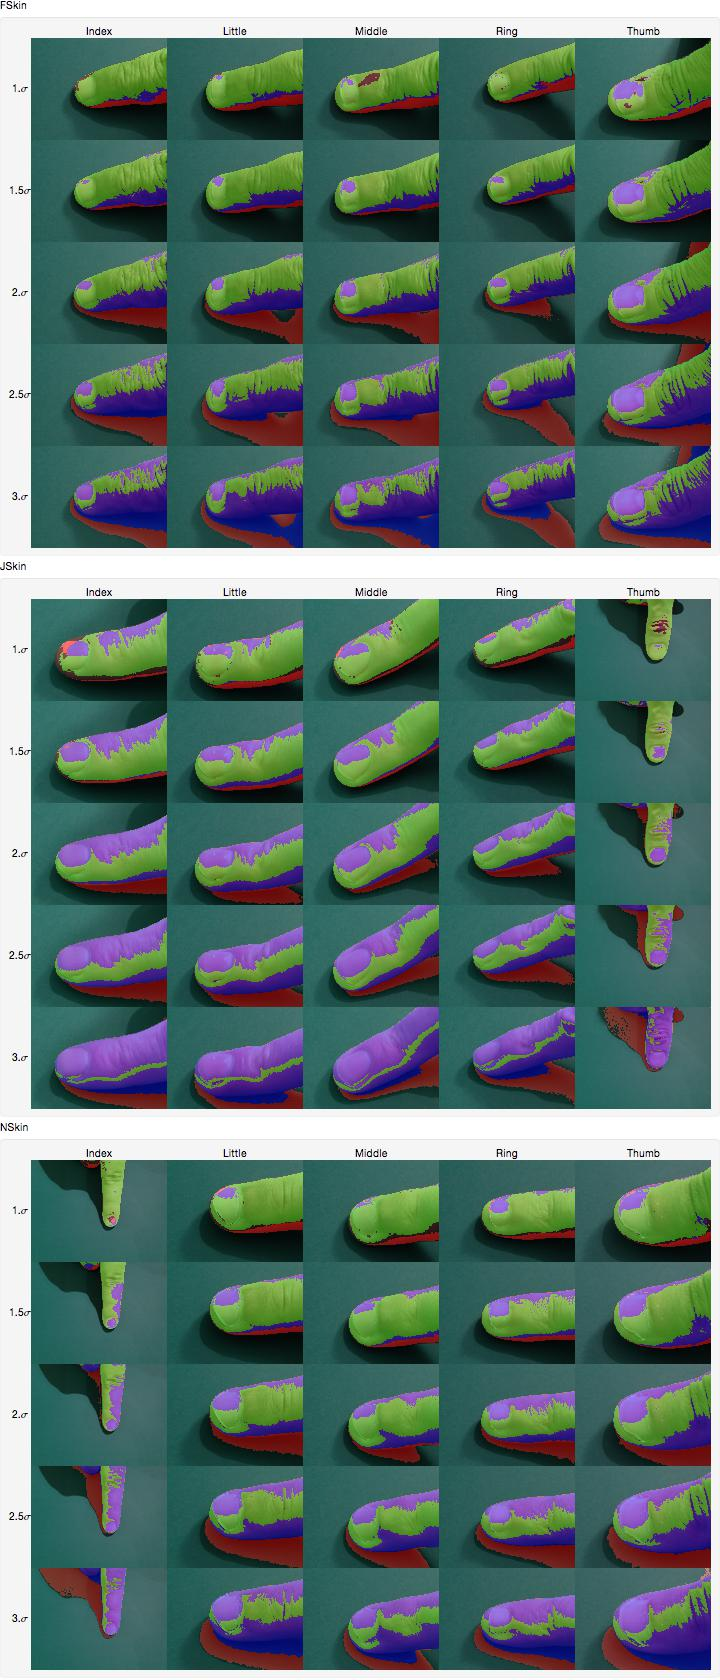
\includegraphics[width=0.85\textwidth,height = \textheight]{Chapter4/Figs/RelaxingSigma.jpg}
      \caption{A selection of images classified using the trinary method outlined in section <so-and-so>, with various values of $\sigma$. It can be seen that $1\sigma$ correctly classifies the majority of pixels, however it classifies some on-digit pixels as "probably not skin", and even "not skin". $3\sigma$, meanwhile, includes large portions of shadow as "probably skin". A compromise of $2\sigma$-$2.5\sigma$ is therefore suggested.} \label{fig:RelaxedSigma}
  \end{figure}
  \clearpage
  }
  
  The standard deviation found in Chap 3 is a very tight fit to the chromatic values taken under controlled lighting conditions. For our practical implementation, this tight fit needs to be relaxed. This is done empirically by trying out multipliers of the standard deviation $\sigma$ on the image sets. What is desired is a multiplier which relaxes the redistribution such that all the pixel values on a given digit are classified as skin, and all the background is classified as not skin. This is done empirically using the trinary classification presented below (in section <so-and-so>), which accounts for white-out and black-out and classifies the pixel value as "definitely skin", "probably skin", "probably not skin", and "not skin".
  
  Using a value of 2.3 times the original $\sigma$ correctly classifies the pixel values; this was found by observing tables of images similar to those in Figure \ref{fig:2BitImage}. 
  
  
  \subsection{The Color Space Algorithm as Implemented}\label{sec:ColorSpaceAlgorithmAsImplemented}
  Here we present the color space algorithm in a way which most closely resembles the C++ code. The construction of the color space object is described at the end of chapter 2; here, the operation of the algorithm is described.
  
  First, we determine the form of the distribution function for a working type tRange with the source range $srcRange=2^n$  and destination range $dstRange=2^m$ expressed in terms of their bit depths.
  
  \begin{gather*}
  \begin{aligned}
  K & =  2^{m-n}  \quad & \quad  
  \tRange(\theta,\mu,\sigma)   & =  \mathbf{l} \; 2^n \quad & \quad
  \mathbf{l}  & = \min\left\{ 2^{m-n}\delta(\mu,\sigma) \right. ,  \left. \mathbf{L}(\theta) \right\} 
   \end{aligned} \\
   \begin{aligned}
    \tMin(\theta,\mu,\sigma)   & =
   \begin{pmatrix}
      0 \\
    -\mathbf{l}_2 \; 2^{n-1}  \\  
    -\mathbf{l}_3 \; 2^{n-1} \\  
   \end{pmatrix} \quad & \quad
    \tMax(\theta,\mu,\sigma)   & =
   \begin{pmatrix}
    \mathbf{l}_1 \; 2^n  \\
    \mathbf{l}_2 \; 2^{n-1}  \\  
    \mathbf{l}_3 \; 2^{n-1} \\  
   \end{pmatrix} \quad & \quad
     \Scale &=
      \mathbf{l} \otimes
     \begin{pmatrix}
       \frac{1}{3} \\
      2^{1-n } \\
      2^{1-n }  \\
     \end{pmatrix}    \\
   \end{aligned}
  \end{gather*}
  
  Substituting into the distribution function \ref{eq:disFunction} gives us
  
  \begin{equation}
\textbf{dis}(x) =  -\frac{2^n \left(\text{erf}\left(\frac{2 \mu +1}{2 \sqrt{2} \sigma }\right)+\text{erf}\left(\frac{2^{1-2 n} x-\mu }{\sqrt{2} \sigma }\right)\right)}{\text{erf}\left(\frac{2 \mu -1}{2 \sqrt{2} \sigma }\right)-\text{erf}\left(\frac{2 \mu +1}{2 \sqrt{2} \sigma }\right)} \quad \textbf{where} \quad
\begin{array}{rl}
qMin < & x  < qMax \\
0 < &\mu <1\\
0 < &\sigma <1
\end{array}
  \end{equation}
  
  This form takes the result of the rotation directly, however we wish to add the flexibility to adjust the mean and use a lookup table for the values. It is desirable to keep the lookup table as short as possible. The maximum compression of the information without losing relevant information is given by compressing to tRange. The number of values in the lookup table can be reduced by scaling $x$ by a range qtRange, which is chosen to balance lookup table size and computational scaling efficiency.  Noting that $\mathbf{l} <2$, qRsRange can be chosen to be equal to tRange as if $\mathbf{l} =2$, which means that qtRange is a power of two, allowing the scaling to be performed by bit shifting the value of $x_{qt} = x \ll n-2$. However, in the region where the function is applied, the information is preserved at best 2-to-1, so the information density can be reduced by half $x_{qt} = x \ll n-1$. Adjusting the mean changes the bounds on the region to be redistributed such that the form of the function does not change. For this reason, we also define $x$ relative to the bounds, which allows the same lookup table to be used regardless of any adjustment to the mean.
  
    \begin{equation}
  \textbf{dis}(x) =  \begin{cases}
    \textbf{disLU}((x-\Lambda_{1}) qtRange)  & \Lambda_{1} < x < \Omega_{pq1} \\
  \textbf{disLU}((x-\Omega_{pq2}) qtRange)  & \Omega_{pq2} < x < \Lambda_{q2} \\
  \textbf{dis}(x)  & \text{Otherwise}
    \end{cases} \quad \text{where} \quad 
    qtRange = \left(\begin{smallmatrix}
    \cdots \\ 2^{1-n}\\2^{1-n}
    \end{smallmatrix}\right)
    \end{equation}
  
  Aside from these refinements, the algorithm presented in Chapter 2 is used to perform the rotation and redistribution as described. The algorithm proceeds as follows:
  
  \begin{itemize}
  \item Interactively find an adjustment to the mean  $\delta\mu$. .
  \item Set the new distribution parameters
  \item Rotate the pixel value with the $\qR$ matrix. $ pxl_{q} = \qR \cdot pxl_{RGB}$ then $ \frac{- qRsRange}{2} < pxl_{q} < \frac{ qRsRange}{2}$
  \item Partition the rotated values to avoid unnecessary processing of irrelevant information.
  \item Apply any user supplied per-pixel functions to the rotated value and add as extra channels.
  \item Redistribute the rotated values into the destination type.
  \item Apply and user supplied per-pixel functions to the redistributed values.
  \end{itemize}

\section{Pattern Recognition Routines}\label{sec:PatternRecognitionRoutines}
In this section, pattern recognition routines which use the new color space are presented and discussed.

\subsection{Trinary Pixel Classification}\label{sec:TrinaryPixelClassification}

\newcommand{\WoBoBool}{\underset{\scalebox{0.5}{WoBo}}{\mathbb{L}}}
\newcommand{\ColorSquareBool}{\underset{ \scalebox{0.5}[0.5]{square} }{ \mathbb{C} } }
\newcommand{\ColorEllipseBool}{\underset{ \scalebox{0.5}[0.5]{ellipse} }{ \mathbb{C} } }

OpenCV's findContours method takes a binary image and finds the contours in that binary image. However, the problem with this method is that we're thresholding on chromatic values, i.e. using color information to break up the image into blobs in which we're finding the contours. This doesn't take into account the white-out and black-out, which was noted previously. This is done by applying equation \ref{eq:InWoBoRegion} and setting a boolean flag $\WoBoBool$ accordingly. The square partitioning performed earlier in the algorithm also sets a boolean flag $\ColorSquareBool$ to 1 if the pixel is within the target range and to 0 otherwise. These can be combined to produce a 2-bit image which indicates both if the pixel value is in the target chromatic range and the reliability of the classification.
% 

\begin{center}
\begin{tabular}{|c|c|c|c|c|}
\hline
Correct                               & Unreliable      & \multicolumn{2}{|c|}{Image Bit} & \multicolumn{1}{|c|}{\multirow{2}{*}{Comment}}  \\ \cline{1-4}
Color $\ColorSquareBool$ & $\WoBoBool$ & $\ColorSquareBool$ & XOR($\ColorSquareBool$, $\WoBoBool$) & \\\hline
0 & 0 & 0 & 0 &  Definitely not the target \\\hline % & Wrong Color &    Reliable Luminosity 
0 & 1 & 0 & 1  & Possibly the target but shifted. \\\hline % & Wrong Color & Unreliable Luminosity
1 & 1 & 1 & 0  & \begin{tabular}{l} Probably the target but possibly \\ shifted into the target region \end{tabular} \\\hline % &   Right Color &    Reliable Luminosity
1 & 0 & 1 & 1  & Definitely the target \\\hline % &   Right Color & Unreliable Luminosity
\end{tabular}
\end{center}


This produces a 2-bit image. For this purpose, a 2-bit data type was added to OpenCV. The question then is how to use it. Essentially, we have four different states: values which are neither the right color nor in the right region; values which are possibly the right color, but because they're outside the valid region, they've potentially suffered from white-out and black-out and as such they are not reliable indicators for either the start of an edge or the end of an edge; values which are in the right region, but the wrong color, and we are certain that they are not skin; and finally, values which are in the valid region and are of the right color.

The Canny edge detector method is perfect for implementing a decision by setting a high threshold --- our strong criteria --- in the right region in the right color, and a low threshold so that it will continue following an edge across values which are in the invalid region. Whichever value we set the low threshold to depends on the state of the image; we use a lower value if there is ambiguity and a higher value if the result is fairly accurate:
 
\begin{figure}[h!]
  \centering
    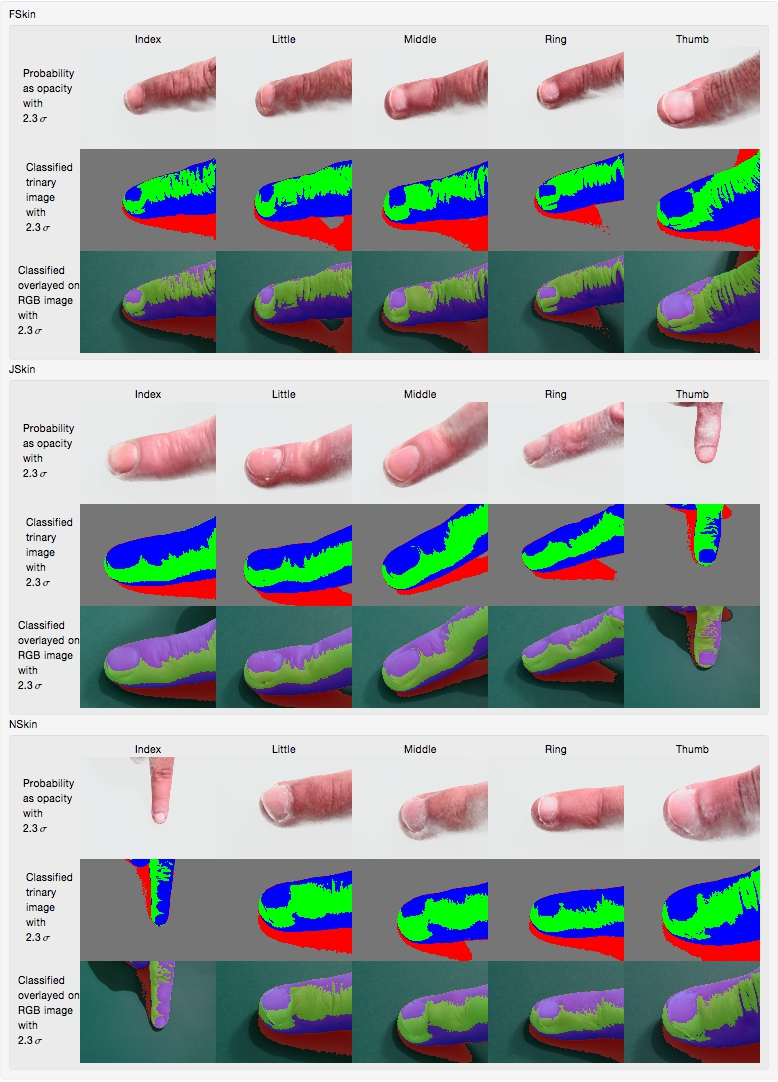
\includegraphics[width=0.95\textwidth]{Chapter4/Figs/ClassifiedSkin.jpg}
    \caption{The Pixel Classification.}\label{fig:2BitImage}
\end{figure}

\subsection{The 'Hurdle' Method}\label{sec:HurdleMethod}
The Hurdle method is an algorithm for finding a path inside an object using the trinary classified image. The Hurdle method follows straight line paths in the object. As written, it is flexible enough to follow any straight line, however the current implementation takes a direction vector and evaluates at multiples of that direction vector. This means that non-horizontal and non-vertical lines are not guaranteed to be continuous. This is because the pixel values are not found using Bresenham's line algorithm. The algorithm has two thresholds --- a high and a low threshold. Whilst the pixel values remain in the high threshold, the path end point variable is updated; when the pixel values are in the lower threshold, the algorithm continues along the path, but without updating the path end point. This allows the path to pass through artifacts (i.e. pixel values which are inside the object but which have been misclassified), but does not allow the path to extend outside of the object into regions which are, for instance, in the shadow of the object.
 
\subsection{The 'Filament Fill' Method}\label{sec:FilamentFill}
The Filament Fill method takes a path --- given as a sequence of points --- within an object and finds the edges of the object using the Hurdle method running away from the path within the object. Assuming a horizontally-oriented object, the path's extent in the horizontal direction is divided equally into points, and these points are used to start the Hurdle method in the vertical directions, and vice versa for vertical-oriented objects.


\begin{figure}[h!]
  \centering
    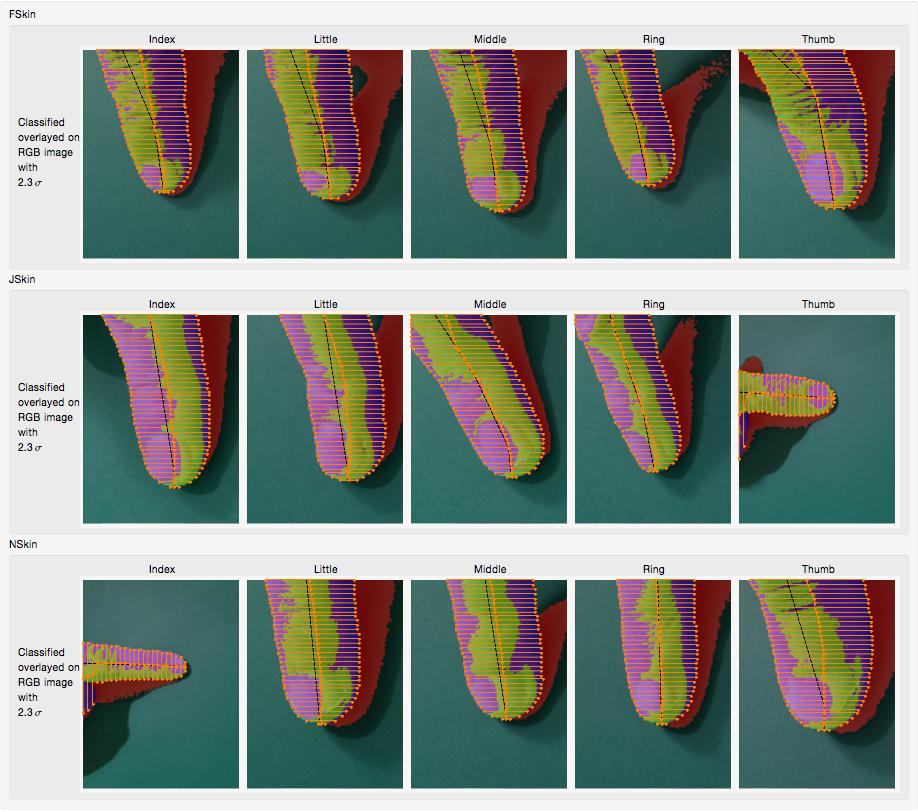
\includegraphics[width=0.95\textwidth]{Chapter4/Figs/FillamentFill.jpg}
    \caption{The 'Filament Fill' Method.}\label{fig:FillamentFill}
\end{figure}

\subsection{The 'Mean-Medians' Method}\label{sec:MeanMedians}
For the purposes of the shape detection algorithms, there are metrics that are applied which suffer from noise and anomalies, where the noise is due to the natural variability of human digits from regular geometric forms, and the anomalies are due to misdetections of the edges of the digit. We assume that the anomalous results are extreme values, however we acknowledge that the most common (mode) or middle (median) values may not be representative of the best geometric approximation for the shape. The Mean-Median method --- similar the "k-Nearest Neighbors" algorithm --- solves this problem by taking a confidence interval around the median and then taking the mean of the points within this interval. This method is a useful adaptation of methods like the k-Nearest Neighbors in that it solves the outlier problem for this particular application.

\subsection{The 'Kink Fit' Method}\label{sec:KinkFitMethod}
The Kink Fit algorithm takes in a set of 2D points, where the first component is taken to be independent variable and the second component is taken to be the dependent variable. This assumption excludes the possibility of truly vertical lines being presented to the algorithm. The Kink Fit algorithm fits a function which consists of two straight-line segments to a set of points. Unfortunately, currently the only piecewise linear fitting function is the proprietary MARS algorithm which, aside from being commercial, is overkill for this particular problem, which has a small number of points which are well-aligned. 

The Kink Fit algorithm relies on the fact that we know that the points are in order; it chooses a point and divides the set in two, and then performs a standard, least squares linear fit to the two sets. Both sets include the point at which the set is divided. 

The fit is also assumed to be continuous, except in the first derivative. The algorithm as described above may produce two lines which do not intersect between the second-to-last data point used for the first line and the second data point used for the second line. The algorithm needs to ensure that this is the case. This is achieved by shifting the second half of the data set by the end point of the linear fit to the first half of the data set. The point at which the two linear fits intersect is found, and if that point is between the second-to-last point in the first set, and a second point in the second set (i.e. the points on either side of the point of division), then the fit is considered to be acceptable. If the fit is not acceptable, it indicates that there's a discontinuity in position rather than simply being a discontinuity in the first derivative. This is handled by choosing the point on the fit to the first set closest to the intersection within the bounds of the points on either side of the point of division. The linear fit is then performed with only the gradient as the free parameter, guaranteeing that the line will have passed through this limiting point.

The algorithm then finds the residuals, and then finds the average of the square of the residuals and adds those averages together. This is considered the score for dividing the set of points at that position. The algorithm finds the point which minimizes the score using a bisecting algorithm; if a linear fit to the data has a low score, then the Kink Fit algorithm is considered unnecessary and the digit is assumed to be in a relaxed, straight, neutral pose. The algorithm specifies a minimum number of points to be included in a set, as this avoids the problem of dividing into sets which contain only one point.

\section{Fingertip Model}\label{sec:FingertipModel}

We need an appropriate finger model so we can accurately align points on the fingertip between successive images in the video stream. We need to do this because otherwise, any difference between the frames will be overwhelmed by physical movement of the digit rather than movement of the blood inside the digit. For this reason, we target the most stable portion of the finger: the nail.

A digit has two joints and three segments: the distal, the middle, and the proximal. Each segment is roughly approximated by a rectangle, and the length of each section approximately following a 2-3-5 ratio, with lengths counting from distal to proximal, and where 1 is the $\frac{3}{4}$ width of the middle segment. Each digit also has a roughly circular feature in the nail close to the tip of the distal segment. Our finger model then comprises of the lengths and widths of each segment, the positions of the joints (i.e. the knuckles) between each segment, the position of the tip, and a position in the model marking the point at which the digit goes out of frame. 

<Now, draw the thing, and show the initial guesses, and where the center is, etc.> 

Given the width of the middle segment, we can then have an initial guess that the length of the distal segment is 1.5 times the initial width, the middle is 2.25 times that, and the proximal is 3.75 times that. Additionally, the center of the nail feature is not in the center of the distal segment, but a half unit (in our model unit) away from the tip. The model can be laid out in units relative to the middle section.
\subsection{The Finger Shape Detection Algorithm}\label{sec:FingerShapeDetectionAlgorithm}

\subsubsection{Scale Space}\label{sec:ScaleSpace}
The images captured with the iPhone camera are extremely large, and so for the development of the algorithm, we define three scale spaces: one is the original image; two is an image size which represents the tip of the finger regardless of the distance of the camera from the finger, i.e. a scale relative to the width of the finger in the frame of the camera; three is a small image size for tracking the finger where it's freely roaming in the camera's view. We want these images to be formed without the need for resampling. For that reason, we restrict the choice of image sizes to those which are integer factors of the image dimensions. This is done by finding the integer factors of the original image dimensions and then selecting from those factors to scale the image. It should be noted that, to simplify point correspondences, the integer scaling from the small to medium scales is also kept.

\subsubsection{Finding the Frame Orientation}\label{sec:FindingTheFrameOrientation}
It is assumed we will not be using severed fingers, and so we know that the finger must exit the camera frame; the first step of the algorithm is then to detect which of the four edges the finger is entering from. This is done simply by finding the longest on-object path running along the frame sides. So, the algorithm stars by looking down the pixels on a frame side; when it locates a high-trinary value, it uses the Hurdle method to find the longest path in that direction starting from that point. It continues around all four sides; the longest path found by the Hurdle algorithm is assumed to correspond to the finger entering the frame. From this, we set a frame orientation, which is the angle necessary to rotate the image such that the finger will be entering the frame from the left, and we set a direction vector pointing inwards from the frame edge found.

\subsubsection{Finding the End of the Finger Shape}\label{sec:FindingTheEndOfTheFingerShape}
Taking the longest Hurdle path on the frame edge found above, we take the middle point on that path and start a "Run-Reach" algorithm in the direction found previously from that point. The Run-Reach algorithm proceeds as follows:

It finds a Hurdle path in the primary direction, i.e. perpendicularly away from the frame edge. At the end of the Hurdle path, it finds the Hurdle paths in the two perpendicular directions to its primary direction, i.e. parallel to the frame edge. It then finds the midpoint between the ends of the Hurdle path, and then uses that to start a new Hurdle path in its primary direction. The algorithm continues in this way until the end of the finger is found.

\begin{figure}[h!]
  \centering
    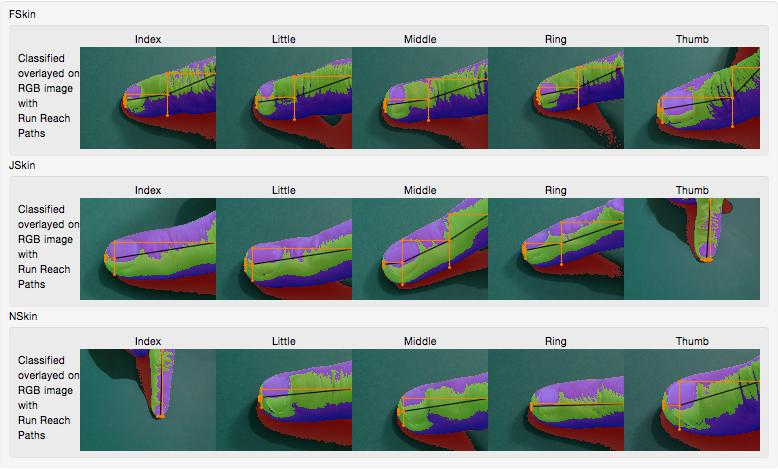
\includegraphics[width=0.95\textwidth]{Chapter4/Figs/FindingTheTip.jpg}
    \caption{Finding the End of the Finger Shape}\label{fig:FindingTheTip}
\end{figure}



\subsubsection{Filament Fill the Finger}\label{FilamentFillTheFinger}
The center points found by the Run-Reach method above form a path on the finger. This is the path given to the Filament Fill method described previously. We now have a set of edge points on the digit. These edge points also have a top and bottom correspondence which, although they're not perpendicularly-opposite points on the finger, they do allow for a midpoint on the digit to be found. This can be seen in Figure~\ref{fig:FillamentFill}.

\subsubsection{Exclude Secondary Frame Edge Points and Fingertip Points }\label{sec:ExcludeSecondaryFrameEdgePointsAndFingertipPoints}
We need to exclude from the calculation of the midpoints on the digit values which are near the tip, and values which touch a second frame edge. This is because values toward the tip --- given that the finger is not necessarily perfectly horizontally-aligned --- give unreliable midpoint values because the Run-Reach path corresponds to shorter and shorter chords on a circle. Values which touch a second edge are, more likely than not, do not correspond to the edge of the digit, but are simply where the digit exits the frame. (For example, JSkin Middle in Figure \ref{fig:ExcludedEdgePointsAndMidlineFit}.)

\begin{figure}[h!]
  \centering
    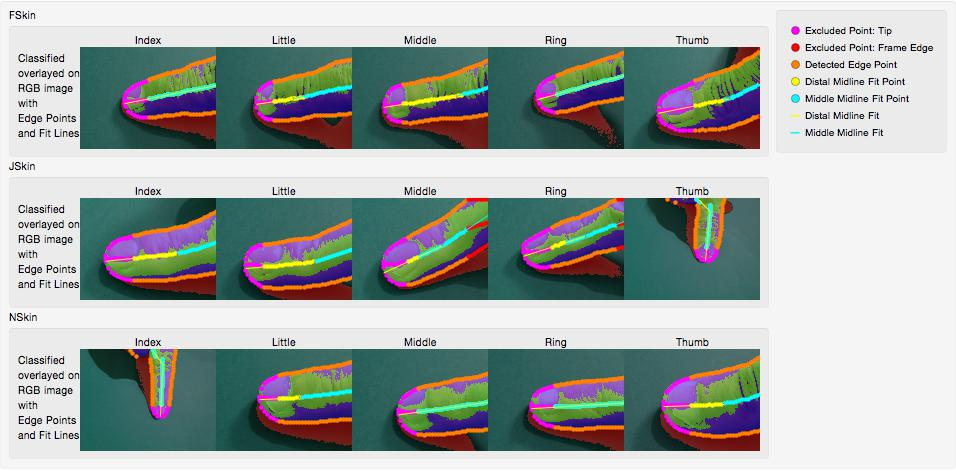
\includegraphics[width=0.95\textwidth]{Chapter4/Figs/ExcludedEdgePointsAndMidlineFit.jpg}
    \caption{Exclude Secondary Frame Edge Points and Fingertip Points.}\label{fig:ExcludedEdgePointsAndMidlineFit}
\end{figure}

To estimate which pairs of edge points corresponds to points on the tip, the algorithm finds the length of the Hurdle path for all corresponding bottom-edge to top-edge points. These values are then sorted into ascending order, and the lowest quarter and highest quarter are discarded, and the mean is taken of the remaining values. This ensures that the average is not affected by extreme values. This method is called the "Mean Median." Values which deviate significantly from this average are regarded to be outliers, or values on the tip. The tolerance is determined by the algorithm by looking at the difference at the low and high ends of the $50\%$ range.

\subsubsection{Kink Fit to the Finger}\label{sec:KinkFitToTheFinger}
We now have a set of reliable points at the midpoint of the finger. Because the finger is articulated, it is reasonable to assume that it may well be bent. Because we're interested in the action of the finger being pressed on a surface, the finger is expected to be articulated at the distal-middle joint, but is otherwise straight. We wish to fit a function which consists of two straight-line segments to the set of reliable middle points. To this end, the "Kink Fit" algorithm was developed. Unfortunately, currently the only piecewise linear fitting function is the proprietary MARS algorithm which, aside from being commercial, is overkill for this particular problem, which has a small number of points which are well-aligned. 

The Kink Fit algorithm relies on the fact that we know that the points are in order; it chooses a point and divides the set in two, and then performs a standard, least squares linear fit to the two sets. It then finds the residuals, and then finds the average of the square of the residuals and adds those averages together. This is then considered the score for dividing the set of points at that position. The algorithm finds the point which minimizes the score using a bisecting algorithm; if a linear fit to the data has a low score, then the Kink Fit algorithm is considered unnecessary and the digit is assumed to be in a relaxed, straight, neutral pose. The score of the straight line fit is taken to be the score of the extreme ends of the division, and the algorithm also sets a minimum number of points to be included in a set, as this avoids the problem of dividing into sets which contain only one point.


\subsubsection{Parallel Lines Fit}\label{sec:ParallelLinesFit}
Our model of a finger assumes that the edges are parallel to each other. Since we have a line which runs through the center of the finger, we can now calculate the distance of the edge points to that line. These distances can be classified as good edge points if they're parallel to the central line. Whether they are parallel is determined by finding the Mean Median distance from the central line to the edge points using a $50\%$ interval in the distal portion, because it is expected that up to half the points may be in the distal segment, maybe on the tip, and a $75\%$ confidence interval in the middle segment, because we expect fewer than $\frac{1}{4}$ of the edge points to be anomalies. The points are then classified as good if they are of Mean Median distance from the central line. It should be noted that we consider both the top and bottom edges when calculating the Mean Median distance. This technique successfully removes anomalies which are not parallel to the central line.

There is one final step: the points which are classified as good edge points are used to find a linear fit which is parallel to the central line. Finally, the width of the distal and the middle segments is calculated by finding the distance between these parallel lines. This can be seen in Figure \ref{fig:ParallelFit}.

\begin{figure}[h!]
  \centering
    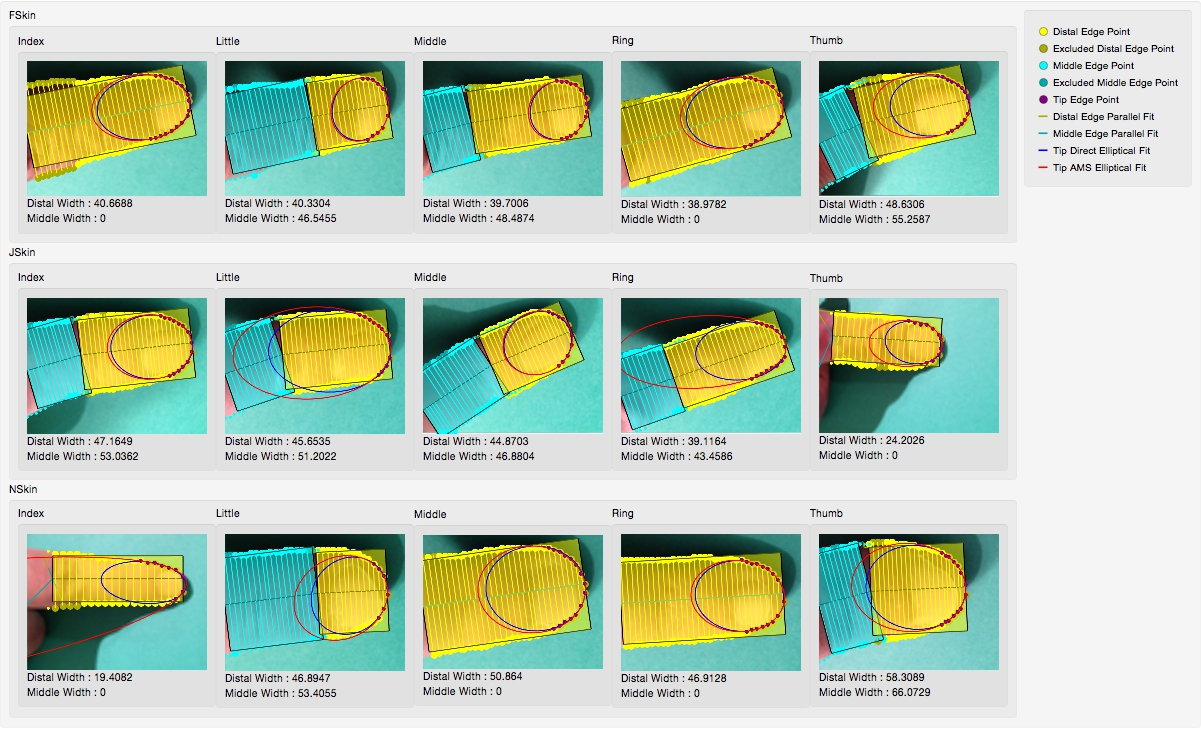
\includegraphics[width=0.95\textwidth]{Chapter4/Figs/ParallelFit.jpg}
    \caption{Parallel Lines Fit.}\label{fig:ParallelFit}
\end{figure}



\

\section{Putting it All Together}\label{sec:PuttingItAllTogether}

So far, we have said little about how we actually intend to detect a digit being pressed on a surface. Although a significant amount of discussion has been presented to do with the optimization --- at least in terms of the data types and the underlying maths --- mostly to do with the color space transform. We have said even less about the size of the images captured or the framerate at which the processing is required. These are important considerations for designing practical code, especially for application in a mobile device.

\subsection{Detecting a Finger Press}\label{sec:DetectingAFingerPress}

In the previous section, we presented several algorithms which perform steps in the task. However, we now need to put them together and fill in the gaps which link each important step together. Assumptions and simplifications which we have allowed ourselves in this work which is intended only to be a proof of concept rather than a fully-fledged application. To this end, we have decided to simplify the requirements and --- although there is no compelling reason why we could not use, say, convex hull and defects to detect the fingers, or even a full hand --- we're only going to consider the case where one digit is presented to the routine in a controlled environment:

The first step in the algorithm is to select a human and a camera. With this done --- using the same camera as will be used by the application --- we gather statistics for a particular individual's skin, trying to vary the lighting conditions so as to give us as representative a data set as possible. From this, a color space is designed and the relevant transforms and such are instantiated for that particular individual.

The next step is to collect the finger features and instantiate the feature detectors using the Canny-edge-based descriptor for each of the individuals' digits.

Now we start the application: it turns on the camera and waits for movement. After the movement starts, it continues to wait until that movement slows, which is the first indicator that a surface is being touched. Here we assume that we are trying to detect static presses, so no pressing and dragging is considered. We look at a higher resolution frame, process that frame into the skin color space for the individual in question. 

Now we perform our shape detector, which looks for a finger-shaped object, finds the tip, creates rectangular bounds for the tip, and then takes an even higher resolution frame. (But only for the tip of the potential finger.) This image --- cropped to the tip of the digit --- is then sent to the feature detecton algorithm, which then uses the Canny edge feature method previously described and attempts to identify the digit by applying the known descriptors for the individual's nail.

These steps are relatively slow, but --- once applied --- the algorithm now only tries to fit one feature descriptor and simply tracks the assumed small movement of the tip during a press. Due to the slow nature of these steps, it's required that the camera buffers a few frames after the motion stops, otherwise the finger press may miss the processing window. It is at this stage that the algorithm to detect the finger press really starts.

Now that the fingertip has been located, the algorithm crops the fingertip before forming the color space transform, which saves a significant amount of processing time. We now define a larger cropping region, and a tight cropping region. The larger of the two cropping regions is used initially to ensure that the entire tip of the digit is captured in subsequent frames, as this cropping region will not vary during the finger press detection stage of the algorithm. Inside the cropping region, a second rectangular region is defined, which is centered using the feature detection, ensuring that the frames are aligned with the true outline of the digit and not the outer pixels. Any change in the tighter frame will be due to the mechanical action on the digit changing its visual appearance.

The tightly-cropped region from each frame is held in as high a resolution as possible, and the absolute distance between each successive frame is calculated in this region. It was discovered that the color channel corresponds to the major axis of the 2D Gaussian fit to the chromatic space. It has been found that a finger press changes the chromatic values in the end of the digit sufficiently for this to register clearly in this region. For the purposes of this project, this difference is calculated and output as an image. However, for the actual application, all that is required is a measure of the size of the change in the chromatic space.

\begin{figure}[h!]
  \centering
    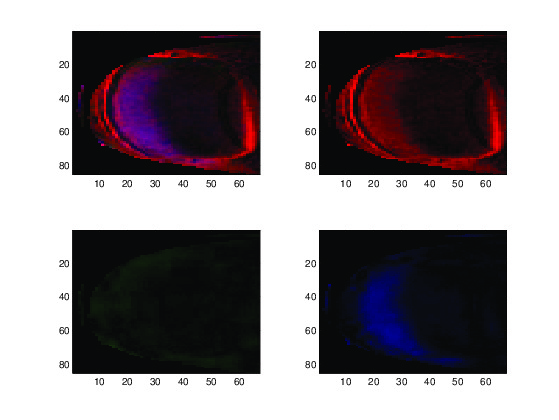
\includegraphics[width=0.90\textwidth]{Chapter4/Figs/jThumb_Final_Proof.jpg}
    \caption{The difference in the skin color space between successive frames during a finger press. (Or in this case, a thumb.)}\label{fig:FinalProof}
\end{figure}

The second indicator for a finger press was found around the center of the pad of the digit. The distance to the convex hull --- which outlines the edge of the digit in the frame --- was noted to move away from the centered reference point. This is because the nail does not significantly deform under mechanical stress, however the soft tissue underneath does. This provides a second level in the metric for detecting a digit press.

The algorithm now decides based on thresholds which could be trained, but in the present implementation were set manually, one on the chromatic difference in the feature region (i.e. the nail), and the second on the contour from the shape detection. The output of each combined to produce a sound, the idea being the harder you press, the louder the noise.

The final step is to detect when the digit starts moving again. Failure of the feature detector to re-align the small frame makes the algorithm start tracking motion again. It looks at the low-resolution frames and sees if significant movement is occurring in the larger frame. It should be noted that the algorithm does not process outside of the larger cropped region during the finger press detection phase.

\section{Skin Detection}\label{sec:SkinDetection}

With the image in the skin color space, skin detection is a significantly simplified problem; the average skin color is at the halfway point in both of the chromatic channels and the Gaussian distribution has already been applied, meaning that performing an elliptical thresholding in the normal color space is equivalent to a rectangular thresholding in the skin color space. The probability distribution can be obtained by combining the distributions in each chromatic channel. Because the thresholding levels in each channel are equivalent to the same points on the Gaussian, they can be straightforwardly combined, and then a single threshold used on the one resulting channel. This can be done by subtracting $\frac{1}{2}$ from both channels, squaring them, then adding them together.

The next step is to identify the skin. For the purposes of this project, we're searching for a skin-colored object of a specific shape: a finger that comes into the frame, presses down on a surface, then exits the frame. One of its properties is that it meets the edge of the frame, appearing as a rectangle with a rounded end which --- on occasion --- can appear slightly bent due to the viewing angle or pressure placed on the finger as it presses down on the surface. But there's a limit to how great that deflection can be in the image.

In order to find this shape, we begin by finding the contours in the binary probability image. This can be achieved by using the "findContours" method in OpenCV, which finds the contours and returns them as a vector of points. In the skin color space, finding the contours around the finger is very simple.

\begin{figure}[h!]
  \centering
      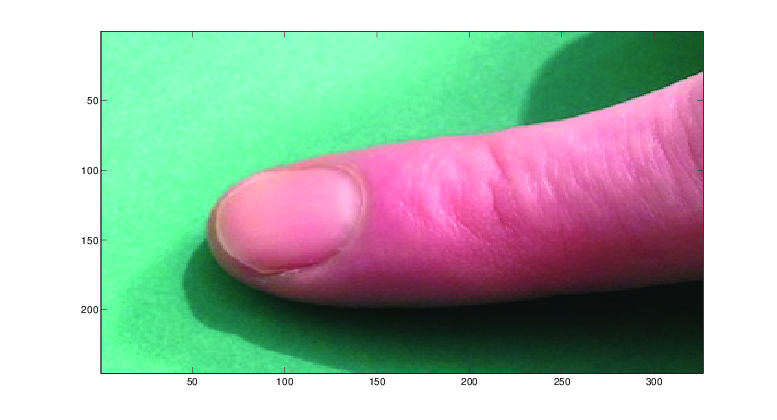
\includegraphics[width=0.45\textwidth]{Chapter4/Figs/imgJIndex1.jpg}
    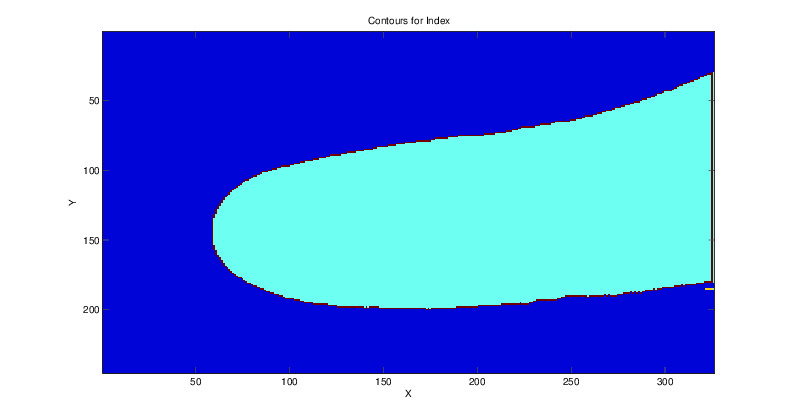
\includegraphics[width=0.45\textwidth]{Chapter4/Figs/indexContours.jpg}
    \caption{Finger contours in the probability image.}\label{fig:IndexContours}
\end{figure}

Once the contours have been identified, a rectangle is drawn around the finger using OpenCV's "rectangle" method, with the tip of the finger touching one of its sides. Next, lines are drawn along the sides of the finger using the "line" method, and a convex hull identifies the semicircular fingertip, again using an OpenCV method, in this case "convexHull." This produces a set of verteces which allow us to locate the fingernail, at which point we highlight it with a square drawn using the "rectangle" method once more. The fingernail image within this square is then sent to the edge detector method for further processing. (See Figure 2.17.)

It should be noted that --- in the finger images in Figure~\ref{fig:IndexContours} --- the finger is deformed slightly due to the application of pressure on a flat surface, as was discussed previously. This doesn't necessarily share the same orientation as the tip. This can be remedied by taking the portion of the image highlighted by the rectangle and performing the operation again, thereby producing a rectangle which is properly oriented with the fingertip.

Once the fingertip has been identified, its features are obtained using the SURF algorithm method provided by OpenCV's SURF class. An initial attempt was made to use the library functions in OpenCV, however the high resolution and the relative uniformity of the fingertip resulted in no stable feature points being automatically detected. The initial idea was to allow the automatic descriptor generator to use a set of aligned frames and the idea was to keep the features which were stable in time and space. (i.e. Present in every frame and in the same location.) This attempt was unsuccessful, so a bespoke method was designed instead.

\begin{figure}[h!]
  \centering
    \includegraphics[width=\textwidth]{Chapter4/Figs/shapeDetection.jpg}\label{fig:shapeDetection}
    \caption{Shape detection in action.}
\end{figure}

\begin{figure}[h!]
  \centering
    \includegraphics[width=\textwidth]{Chapter4/Figs/rainbowmanRGB.jpg}
    \caption{RGB channels.}
\end{figure}

\begin{figure}[h!]
  \centering
    \includegraphics[width=\textwidth]{Chapter4/Figs/rainbowmanRotated.jpg}
    \caption{Rotated color space.}
\end{figure}

\begin{figure}[h!]
  \centering
    \includegraphics[width=\textwidth]{Chapter4/Figs/binsFinal2.jpg}
    \caption{Final bins.}
\end{figure}

\begin{figure}[h!]
  \centering
    \includegraphics[width=\textwidth]{Chapter4/Figs/rainbowmanRotatedScaled.jpg}
    \caption{Rotated and scaled color space.}
\end{figure}

%%*****************************************************************************************
%*********************************** Fourth Chapter **************************************
%*****************************************************************************************

\chapter{Future Work and Discussion}

\ifpdf
    \graphicspath{{Chapter5/Figs/Raster/}{Chapter5/Figs/PDF/}{Chapter5/Figs/}}
\else
    \graphicspath{{Chapter5/Figs/Vector/}{Chapter5/Figs/}}
\fi
\section{Results and Evaluation}\label{sec:ResultsAndEvaluation}

All the performance gains are made in the work of Chapter 2, in which we presented an integer-based method for performing the color space conversion which we hoped would be a bit more efficient in comparison with the standardly-used floating point method. To compare the two methods, an equivalent floating point color space conversion method was implemented which first converted the pixel value into a double precision unit range, performed the rotation using a double precision rotation matrix and then redistributed with the redistribution function described in Chapter 2 to the destination integer range. This is compared below with the optimized integer method presented in Chapter 2.

\subsection{Timing the Methods}\label{sec:TimingTheMethods}

Because we have multi-core CPUs running operating systems which handle multi-threading, even on mobile devices these days, it is problematic getting clean running times for algorithms on such modern devices. In investigating this, the two algorithms were run using the same input 1,000 times. Theoretically, the time should be the same for every run with the same input, however, as can be seen in Figure \ref{fig:TimingVariationPlot}, the timings vary away from a baseline with a statistical positive error. It is reasonable to assume that this variation is due to interrupts from system processes, and so the algorithm performance is best measured by taking the minimum runtime from this set of 1,000 runs. 

For the image used in this test, it can be seen that the integer method is about 4.9 times faster than the floating point method. This is a significant gain given that the color space transform is the most computationally-intensive operation in the entire algorithm.

\begin{figure}[h!]
  \centering
    \includegraphics[width=0.95\textwidth]{Chapter5/Figs/Timing_Variation_Plot.jpg}
    \caption{Timing variation plot. Comparison of process run times using the floating point method and the integer optimized method with the same image input data.}\label{fig:TimingVariationPlot}
\end{figure}

\subsection{Optimization Variation with Input}\label{sec:OptimizationVariationWithInput}

Now we evaluate the performance of the algorithm with differing input images. For the purpose of this test, images generated with varying tonal characteristics is done by generating images with random pixel values within random ranges. Each image was processed 1,000 times and the minimum runtime from those 1,000 runs was taken to be an indication of the difficulty of that image when presented to the two algorithms. The algorithms were run over 100 different images, and the mean and the standard deviation from that mean were found for each of the two methods. The performance of the algorithms can be seen in Figure \ref{fig:ToneVariationPlot} below.

\begin{figure}[h!]
  \centering
    \includegraphics[width=0.95\textwidth]{Chapter5/Figs/Tone_Variation_Plot.jpg}
    \caption{Tone variation plot.}\label{fig:ToneVariationPlot}
\end{figure}

Here the performance gain can be seen to be slightly lower than for the test image used above. However, it can be confidently said that the method presented in Chapter 2 is 4-5 times faster than using the usual floating point methods.

\section{Future Applications}\label{sec:FutureApplications}


\subsection{Medical Applications}\label{sec:MedicalApplications}

One possible application of the algorithm is monitoring inflammation. By adapting the color space to distinguish between healthy and inflamed tissue, one might be able measure the degree of inflammation over a period of time by, for the sake of example, photographing parts of the user's body prone to inflammation throughout the day and using the algorithm to perform the comparison. This has the benefit of measuring the degree of inflammation without having to rely on subjective reporting, and could allow individuals to discover triggers for conditions like eczema, arthritis and other such inflammatory diseases. Combining this approach with diet and lifestyle monitoring functions --- other factors which may contribute to inflammation --- could serve as a simple and empowering means of increasing users' quality of life.

In mole mapping, a series of photographs of moles are taken over a period of time to track changes in size, color or shape in order to detect conditions such as malignant melanoma. However, identifying changes in such skin lesions is often limited to the doctor performing naked-eye comparisons between RGB photos of the areas of concern. (Figure \ref{fig:MelanomaImages}.) This poses a problem when checking for changes in color, in part due to the RGB color space not separating the luminosity from the chromatic information and differences in lighting conditions. Using our color space, it is possible to highlight such changes more clearly; the color space can be adapted to detect changes in coloration between successive skin lesion images, thereby eliminating the need for guesswork. Additionally, by floating the mean the algorithm can account for variable lighting conditions.

Blood flow patterns in the retina are a good indication of eye health. As such, a retina imaging app for monitoring these blood flow patterns is another potential application of the algorithm. It is possible to adapt the color space to discriminate between oxygenated and deoxygenated blood flow and use the image alignment such that, with a simple lens manipulator which fits over the phone's camera, one could photograph their own retina daily and measure the difference overtime. The alignment algorithms could be used to monitor any burst blood vessels, even within the eyeball itself. Another, similar application would involve detecting for anemia; the skin under the eyelids lacks pigmentation, appearing pale if there is little blood. One might be able to take a photo of the skin under the eyelids with their phone camera and use the algorithm to check for a lack of blood flow.

As for applications beyond phone cameras, a number of different medical cameras have been designed for medical diagnostics (see Figure \ref{fig:MedicalExaminationCameras}), especially for use in telemedicine and thermal imaging, and many of which are commercially available. These cameras are typically HD video cameras, some of which support a variety of attachments for different types of examinations such as tongue depressors for laryngoscopy. However, these cameras also tend to use the RGB color space, which again has the disadvantage of requiring the examiner to perform a naked-eye comparison, relying on their knowledge and experience to make a diagnosis. By adapting our color space to target specific chromophores, it may be possible to accurately diagnose any number of conditions without relying as much on expertise. 

Also, the use of lossy methods; our color space can keep all the information, so better. Differences in chromophores like oxyhemoglobin and deoxyhemoglobin and the two types of melanin are very small, so losing information makes telling them apart that much harder.

Another benefit of using the algorithm is that it's lossless; unlike the lossier methods used in many medical applications, our color space retains all the chromatic information without negatively affecting performance. This is especially beneficial when performing comparisons between chromophores with very subtle differences such as oxyhemoglobin and deoxyhemoglobin or the two types of eumelanin, as losing information makes telling them apart that much harder.

\begin{figure}[h!]
  \centering
    \includegraphics[width=0.45\textwidth]{Chapter5/Figs/DermLite-DL1.jpg}
    \caption{DermLite DL1; A dermatoscope attachment available for several smart devices, used in diagnosing skin disorders.}\label{fig:DermatoscopePhone}
\end{figure}

\begin{figure}[h!]
  \centering
    \includegraphics[width=0.45\textwidth]{Chapter5/Figs/melanoma-images.jpg}
    \caption{A skin lesion photographed under different lighting conditions. (Photos by Kevin Jakob, Illingworth Research.)}\label{fig:MelanomaImages}
\end{figure}

\begin{figure}[h!]
  \centering
    \includegraphics[width=0.45\textwidth]{Chapter5/Figs/TEHD_1.png}
    \includegraphics[width=0.45\textwidth]{Chapter5/Figs/examination-clinical-dermoscan-x2.jpg}
    \caption{A few different medical examination cameras. }\label{fig:MedicalExaminationCameras}
\end{figure}

\subsection{Scientific Applications}\label{sec:ScientificApplications}

\subsubsection{A Study of Human Chromatic Diversity}\label{sec:AStudyOfHumanChromaticDiversity}
In Chapter 3, we used a sample set of skin images from three individuals; it was interesting to see, in the lumiochromatic color space LCaCb, how close these skin statistics were to each other in the chromatic plane. It would also be interesting to perform the work of Chapter 3 for a large and chromatically diverse group of people. An attempt was made to look at a diverse sample of individuals using images collected in the Humanae project (\cite{dass2012}). This failed, however, as we had no control over the camera or the image compression performed before making them available on the Internet. Ultimately, it would be interesting to see if it were possible to estimate the levels of the skin chromophores identified in Chapter 1 using the skin statistics of the individual.

\subsubsection{Chromatic Statistics for Injuries and Defects}\label{sec:ChromaticStatisticsForInjuriesAndDefects}
If we have the normal skin statistics for an individual, we could take images of a site of injury and build the chromatic histogram (Figure \ref{fig:Fill_the_Bins}). We could find the difference between the sets and create a profile for the injury or defect. In order to do this, it would be useful to have built the statistics for the injury site prior to injury; this is an issue of this is to be done in-lab as it would necessitate causing the injury or defect in order to study it. This could be overcome using crowdsourcing. For instance, one might go skydiving as a hobby so often bruises their legs, so we could build the skin statistics for their uninjured skin and simply wait for a bruise to appear. 

An issue of this approach would be the consistency of lighting conditions; this could be overcome if we have adapted the method to allow us to set a new white point as outlined in Section \ref{sec:GeneralizingTheRotation}. We could take an uninjured skin patch for which we already have a previous image from which we build the skin statistics, and comparing the two would allow us to find a white point which accounts for the ambient lighting conditions. Our generalized transform could then compensate for the changing lighting conditions. Any difference in the statistics now is due to the injury, and our theoretical model built in Chapter 1 should allow us to interpret this in terms of the chromophores, the key one being the bilirubin, which is a chromophore which causes the yellow-and-green coloration in bruises.

\subsubsection{Repetitive Strain Study}\label{sec:RepetitiveStrainStudy}
The algorithm we developed in Chapter 4 focuses on the mechanical stress to the fingertip when pressing on a surface; in the Figures \ref{fig:ICWaSResultJSkin}, \ref{fig:ICWaSResultFSkin} and \ref{fig:ICWaSResultNSkin}), it can be seen that the stress also shows in the knuckle. In fact, the mechanical strain can be seen in all the joints of the hand. This suggests that we could build an algorithm which monitors the stress in the joints of the hand by observing the blood flow using the routines developed above. By monitoring the strain put on the joints of an individual's hands while they perform a task, we could measure the overall strain that they have placed on their finger joints. If we combine this with the techniques to measure inflammation presented in Section \ref{sec:MedicalApplications}, we could get a measure of the damage suffered by the individual. 

Once developed, such a monitoring system could be used in studies which assess different ergonomic designs and workplace practices. 

\subsection{Computer Vision Applications}\label{sec:ComputerVisionApplications}

\subsubsection{A Novel Canny Edge Detection Algorithm}\label{sec:ANovelCannyEdgeDetectionAlgorithm}
The trinary classification developed in Chapter 4 can also be used for an edge detection routine which operates similarly to the Canny edge detection. The Canny edge detection operates by finding edges using a high threshold which is then lowered as the routine traces along the edge, allowing the edge to be extended from a strong edge into a weak edge. This also allows Canny edge detection to "hurdle" over minor defects in the image of the edge. The trinary classified image can be binarized and presented to standard edge detection techniques, thus we can find all of the strong edges. 

The edges which end surrounded by possible "probably not skin" values can easily be found and marked. Other marked ends which lie close to each other are joined if the pixel values on the path between them are all "probably not skin" (1) or higher. This is similar to the Canny edge detection in that it allows us to join edges by using a lower threshold across the joint. It differs from Canny, however, in that it does not allow the edge to extend into a lower threshold edge. This would be undesirable using the trinary classification because the low threshold "probably not skin" classification often appears in patches which extend across the true edge often resulting from shadow or reflection. This method could be refined by taking into account the orientation of the edges at their end points, which could be used to determine how if the edges should actually be connected. This is similar to the "hurdle" method presented in Section \ref{sec:HurdleMethod}, but applied to edges.

\subsubsection{Finger Feature Detection}\label{sec:FingerFeatureDetection}
The modeling techniques developed in Chapter 4 can be relatively straightforwardly extended to model the entire digit, or even the whole hand. In Chapter 4, we found that the distal width could be used to find a good estimate for the position of the knuckle using the distal, middle and proximal ratios. With this initial model, the next question is what features can we expect to find at these positions in the image? The luminosity axis shows a striking feature at the knuckle position: the knuckle wrinkles. These wrinkles are consistent to each knuckle (i.e. when flexed, they presented in the same way), and they're easily identified by orientation, running across the digit as opposed to along it. Additionally, the knuckle wrinkles curve around the center of the knuckle. This could be used to refine the model and track the knuckles. In the chromatic channels, they also display blood flow when flexed.

\section{Color Space Algorithm Improvements}\label{sec:ColorSpaceAlgorithmImprovements}
Here we suggest several improvements which could be made to the color space algorithm developed in Chapter 2. The improvements presented herein address generalizing the algorithm to accommodate the characteristics of cameras other than the iPhone's. We consider three adaptations; one to allow for multi-spectral cameras, another to allow for cameras which do not have a fixed white point, and a third to handle RAW images captured from the CCD without the iPhone's pre-processing. In practice, these three adaptations need to be combined. Hopefully it shouldn't be too difficult to imagine how this could be done, but in terms of practically proceeding, each one would need to be tackled individually first.

\subsection{Generalizing the Rotation}\label{sec:GeneralizingTheRotation}
In Chapter 2, we derived an expression for a rotation matrix consisting entirely of integers which rotates the RGB pixel values into a custom color space with a luminosity axis and two chromatic axes. The orientation of the chromatic axes is specified using a free rotation $\theta$ about the luminosity axis. The only restriction on the free parameter $\theta$ is that which results from the requirement for the matrix to consist entirely of integer values within a specific range. The question remains: is it possible to achieve a similar result without restricting one of the axes?

In this work, we assumed that an 8-bit per-channel value of $(255, 255, 255)$ corresponds with white. This, however is a result of the pre-processing on the iPhone. Extending this work to other devices or accessing the iPhone's RAW camera feed, it may be desirable to use a different point for the camera's white point. Another reason is to adjust for local ambient light conditions; it is common in digital photography to choose a pixel value from a reference white object to set a white point for the image, allowing a color correction to be performed.

An arbitrary rotation is determined by three angles, and so it's conceivable that the work of Chapter 2 (Section \ref{sec:ConstructingANewColorSpace}) could be repeated for this arbitrary rotation. Whilst it may be possible, an alternative approach may be preferable given the complexity of the general rotation equations. First we assume that the solution exists, then form an initial guess at the solution by quantizing the floating point representation of the matrix. Next, we find the maximum error produced by our approximate quantized rotation by rotating the corners of the RGB cube and comparing the results, then numerically search around this approximation for improvements. The question that remains is what search area should be included.

<math here>

Because the general rotation matrix can be split into the product of three individual matrices, each of which is dependent on only one of the three free parameters, the work in Section \ref{sec:ConstructingANewColorSpace} could be repeated relatively straightforwardly for each of these three individual matrices, and from this --- for a given quantization criteria --- a minimum and a maximum angle step size (Figure \ref{fig:PtbToChan}). If we have for the separate matrices a minimum and a maximum step size, it's a reasonable idea to search around our initial approximation in steps of the minimum step size to either side out to a maximum distance of the maximum step size. For each of the three angles, we search within a cube with sides defined by the maximum step sizes for each of those rotation matrices. On a cubic grid defined by their minimum step sizes. The result of this is that there is a relatively small set of possible optimized choices. Although this is not solving the problem to the same degree that was done in \ref{sec:ConstructingANewColorSpace}, where we reduced it to a mathematical function, it provides a practical way of achieving the same results without excessive computational effort in the setup. 

\subsection{Multi-Channel Color Spaces}\label{sec:MultiChannelColorSpaces}

As mentioned in Chapter 1, the RGB color space is an approximation to the full spectrum of light. However, cameras which are not confined to the three-channel approximation are becoming commercially available (Figure \ref{fig:MultiSpectralCameras}); such a multi-channel image contains far more information about the objects in frame. So where the camera is being used for computer vision tasks where the objective is not to produce a pretty picture to present to the human eye, this allows the chromatic space to discriminate between different objects and surfaces in ways which are unseen by the standard RGB camera point of view.

\begin{figure}
  \centering
  \begin{tabular}{cc}
  \subfloat[Triwave EC701.]{
    \includegraphics[width=.49\textwidth]{Chapter5/Figs/multispec-triwave.jpg}
    }&
  \subfloat[HyperCam by University of Washington and Microsoft Research.]{
    \includegraphics[width=.49\textwidth]{Chapter5/Figs/multispec-hypercam.jpg}
    } \\
    \multicolumn{2}{c}{
    \subfloat[Optec multi-spectral camera.]{
        \includegraphics[width=.49\textwidth]{Chapter5/Figs/multispec-optec.jpg}
    }
    }
  \end{tabular}
  \caption{A variety of multi-spectral cameras currently in use.}
  \label{fig:MultiSpectralCameras}
\end{figure}

The basic design of these multi-spectral cameras is essentially the same as for the RGB cameras where the spectrum of light on each point in the scene (roughly speaking, see Chapter 1) is represented by a combination of Gaussians, the only difference being we have more Gaussians. Each channel can therefore be considered an orthogonal axis in a multi-dimensional color space. The multi-dimensional color space contains a point which corresponds to white, so it is just as possible to construct a color space with a luminosity axis and $n-1$ chromatic axes for an $n$-channel image. Transformation to this color space is defined by a multi-dimensional rotation; this rotation could be optimized in a similar way to that presented in Chapter 2. However, our requirement in Chapter 2 was that the immediate result of the rotation would fit into a data type no more than twice the bit depth of each channel. An $n$-channel color space will be rotated by an $n$ x $n$ rotation matrix; if we have $m$ bits per channel and the quantized rotation matrix is expressed in $l$-bit integers, the result is $l + m + (n-1) \leqslant 2m$. For the larger values of $n$, the rotation matrix would have to be expressed in smaller data types, so aside from special rotation angles which just happen to produce integer rotation matrices, it's unlikely that our criterion can be met. So for multi-channel images to still be able to use integer rotation matrices, the target data type will undoubtedly have to be significantly larger. 

\subsection{Using the RAW Image From the Camera}\label{sec:UsingTheRAWImageFromTheCamera}
The RAW camera image contains all the information captured by the camera, but without any pre-processing. Individual CCDs have different sensitivities in each of their channels, and so the corresponding bit depth of each channel may actually vary. This is likely to be the case for the iPhone's camera as we found in Chapter 3 that certain RGB values appear to be inaccessible. These inaccessible values also appear to be relatively evenly-spread throughout the RGB cube, which produced what we referred to as "speckling" in the statistics gathered in Chapter 3 as seen in Figure \ref{fig:Despeckle_the_Bins}. 

A possible explanation for this is that one or more of the iPhone camera's channels are not truly captured at an 8-bit depth, but a smaller range of values which the CCD actually captures is stretched to fit the full 8-bit range. It is also entirely possible that one or more of the channels may actually be captured at a higher bit depth than 8-bit. But in terms of the algorithm, we now need to allow each channel in the source to have a variable bit depth. This will affect several things; it changes the integer range of allowed values in a rotation matrix and the algorithm for determining the optimal angle could be adapted by weighting the channels appropriately. But otherwise, adapting to a RAW camera image should be relatively straightforward.

\section{Implementation Improvements}\label{sec:ImplementationImprovements}

\subsection{An Empirical WoBo Algorithm}\label{sec:EmpicialWoBoAlgorithm}
The White-out Black-out algorithm outlined in \ref{sec:WhiteoutAndBlackout} uses theoretical values based on the extent of the data type used to store the RGB image. Looking at the empirical results presented in Figure \ref{fig:WhitePoint}, there's more to the WoBo behavior than simply saturating the data type; the performance of the CCD changes with overall ambient light, and the pre-processing performed on the device also has an effect which takes the pixel values away from the naive data point values using the data type extent. 

Although it may be possible to reverse-engineer both the pre-processing and CCD characteristics simultaneously, this would be a difficult task at best. However, if for a device we were able to obtain the RAW image from the CCD, then repeatedly performing empirical tests, such as those performed to generate Figure \ref{fig:WhitePoint}, the CCD characteristics could be obtained. If we know how the CCD detects objects of a certain color under different ambient luminosities, then a more nuanced algorithm can be used to determine if a certain pixel value has suffered from white-out or black-out.

\subsection{Auto-Adjusting the Variance}\label{sec:AutoAdjustingTheVariance}
The algorithm presented in Chapter 4 uses a reference image to float the mean, yet algorithm makes no attempt to adjust the variance to local ambient light conditions. This is found to work well, however it was initially found that using a standard deviation 2.3 times larger than the value found in Chapter 3 produced better results. (See Figure \ref{fig:RelaxedSigma}.) Although the algorithm was tested against a selection of background colors which are notably close to skin colors were avoided. For practical applications, it may therefore be useful to use a value for the standard deviation close to that used in Chapter 3.

The image is chosen to be included in this document were taken against a green background because that gave the cleanest results; a value of 2.3$\sigma$ produced good results in this ideal background condition, so we'll choose 2.3 as the overall upper limit and 1$\sigma$ as the overall lower limit. We have a reference image where we have a good idea that there is a finger, and a portion of that finger is within a known frame, so the lower criteria is that nearly all, if not all, the pixel values within that frame are categorized as skin using the new value for the standard deviation, so for a choice between 1$\sigma$ and 2.3$\sigma$, we can "score" the choice as follows:

\begin{enumerate}
\item The proportion of pixels within the known skin region successfully classified as skin.
\item The number of edge points found using the Filament fill algorithm which are classified as bad edge points which also lie outside the approximated digit edge.
\item The number of edge points found by Filament fill which are classified as bad edge points, but which lie within the edges of the digit.
\end{enumerate}

So, a score where measure 1 is too low suggests that $\sigma$ should be increased, as pixel values which we know to be skin are classified as not skin; if measure 2 is too high, then we need to reduce the value of $\sigma$; and if measure 3 is too high, then we need to increase the value of $\sigma$.

This suggests a way that an algorithm could be developed which appropriately adjusts the value of $\sigma$ striking a compromise between false negatives and false positives. The actual values, thresholds and criteria used can best be determined empirically.

One way of proceeding may be to combine the three measures by taking the weighted product of measures 2 and 3 with the weighted reciprocal of measure 1. We combine the measures in this fashion and minimize the result with respect to $\sigma$.

\subsection{Statistics Gathering Method for the App}\label{sec:StatisticsGatheringMethod}
Given that, in the implementation, we have "floated" the mean and "relaxed" the standard deviation, and above, a method is suggested for adaptively adjusting the standard deviation, it is natural to consider whether the app can handle all the work from Chapter 3. Collecting the statistical model following Chapter 3 is entirely possible, as at no point is any human intervention necessary. However, the Chapter 3 methodology requires that a set of images are captured against a uniform, highly chromatically-contrasting background, which is not a practical or interesting extension to the app.

An interesting possibility is whether the work of Chapter 3 can be somewhat replicated using the same reference image which is used by the app to float the mean and build the initial fingertip model. The difficulties with this idea are the same two difficulties faced by most statistics-gathering methods; sample size and selection bias. To address the first difficulty, we've seen that the number of pixels within the frame which correspond to skin is sufficiently large to usefully adjust the mean of the distribution. This suggests that the sample size should not be a significant problem. Selection bias, on the other hand, comes from asking the user to select a portion of their finger which they consider to be most skin-like; this is not an explicit request of the user, but an implicit request, i.e. when asking a person to supply a sample of skin, they will supply the most skin-like sample they can. This selection bias will likely exclude the edges of the digit, strong features and poorly-lit portions of the skin. As a result, while the mean almost certainly will be fine, the variance will be narrow. So, it's easy to imagine using techniques suggested for auto-adjusting the variance (Section \ref{sec:AutoAdjustingTheVariance}) to make the distribution more inclusive.

One final refinement suggests itself at this point; the resulting color space can be used to model the fingertip and mask the image such that only on-digit pixels are present. In doing this, we now have a broader sample set of pixel values which don't suffer from selection bias. These pixel values could be passed back through the statistical model algorithm to produce a skin chromatic model which is less susceptible to human input.

\subsection{Improved ICWaS Alignment}\label{sec:ImprovedICWaSAlignment}
To align successive frames, the ICWaS developed in Chapter 4 uses OpenCV's template aligning routines which operates by performing a translation of one frame and computing a per-pixel difference. This works because the alignment is already quite good. There are two ways in which this can be improved; the allowed transforms can be increased to include rotation and perspective adjustments, and the alignment methodology can be improved to utilize more constant features of the fingertip image than the per-pixel approach. 

It's a simple matter to allow for a more general transform, however the per-pixel based comparison is wholly inappropriate to find a more general transform as we would have to try all possible results of the transform and compare them. This would be computationally far too expensive. So, to find a more general transform, we must turn each frame into a set of feature points which can be put into a correspondence, or perform some image transform which simplifies the alignment problem.

<figures here>



\subsection{More Designed Metric for Mechanical Stress}\label{sec:MoreDesignedMetricForMechanicalStress}
The metric method which is very briefly presented at the end of Chapter 4 (see Figures \ref{fig:ICWaSResultJSkin}, \ref{fig:ICWaSResultFSkin} and \ref{fig:ICWaSResultNSkin}) relies on a pixel-to-pixel comparison; it is well known that pixel-based methods are unreliable for detecting movement, and our mechanical stress measurement relies on detecting the flow of blood. The metric should therefore account for neighboring pixels. 

There are many possible methodologies for detecting movement which would improve the pixel-based method of Chapter 4. Mechanical stress tends to move pooled blood from one area to another within the stressed tissue. The upshot of this is that as one portion of the image loses blood, another gains it. This is different to the circulatory blood, which is pumped in through the arteries and capillaries and flows out through the veins. A better metric may be to compare blobs in the negative and positive chromatic difference images. To be clear, the algorithm would find blobs using a negative thresholding and a positive thresholding; the largest blobs in each of these spaces would be considered good indicators of pooled blood flow.

Another possibility arises from incidental observations of the pooled blood flow images; for each individual's digit, the pooled blood flow pattern is fairly consistent under similar mechanical stress conditions. This suggests that it may be possible to construct a blood flow model for a given digit. Regarding the app, we can imagine generalizing the reference image idea to asking the user to press on a surface several times, allowing the blood flow model to be generated for that digit.

\section{Conclusion}\label{sec:ConclusionCh5}

The finger press algorithm is really a simple application to demonstrate the viability of detecting blood movement using a standard camera on a mobile device. Many previous authors have dismissed using bespoke color spaces for such applications simply because the color space transform itself is computationally intensive and significantly loses information when applied using standard, off-the-library-shelf color spaces. It's fundamentally difficult to use with the loss of information, with white-out and black-out, and the computational intensity right at the front of the algorithm have meant that such techniques have seen little use.

It is hoped that, with the rigorous optimization of the transform itself --- which is considered in great and incredibly tedious detail in chapter 2 --- that these color spaces can see greater application in the future, although it's recognized that the level of attention that's currently required to make the routine as efficient at the one designed herein will likely be beyond the patience of many practitioners, some of whom are medical professionals and not computer scientists. Also, it is hoped that the work presented here has addressed the concerns about the loss of information associated. This surely must be the case because the color space transform is designed not to lose any information from the RGB color space.

Finally, the use of a Gaussian model for the skin color space has been the source of much debate; some authors insist that the Gaussians be extended to the three-dimensional space, but hopefully it can be seen from this work that a luminosity Gaussian distribution is an artifact due to white-out and black-out, and so is not necessary. The potential gains of using such a luminosity distribution would appear to be gained using the 2-bit Canny edge detection algorithm outlined in~\ref{sec:ImprovedContourDetection}.

The color space algorithm has many possible future applications as an aid to diagnostics, however specialist cameras will always outperform in this area. Also, mechanical stress is not limited to the end of the fingers; knuckles significantly whiten when flexed, so the color space could aid in hand posture work, as would the Canny edge detection methods --- although not presented here during the design of the algorithm --- it was striking how clearly other hand features presented themselves. For instance, it was very tempting to attempt to attach a feature descriptor to the perpendicular creases in the knuckles.

Although not presented here, the majority of the time and effort involved in producing this work went into the furthering of the OpenCV library, which is an open source project hosted on GitHub. The reason this occupied so much of the time is because, at the start of this project, there was no working implementation for iOS. Additionally, the new C++11 standard was released and many of the associated libraries were upgraded, as is so oftenthe case with computer science projects, a significant amount of time had to be dedicated to actually making the code and the libraries work on the selected device appropriately. Probably the most significant contribution this project has made to the library is the extension of the internal data types, which were necessary both for the C++11 standard and the 2-bit and 4-bit types which allowed for the optimization of many of the heavy-duty routines.

As for the finger pressure detector, it could be extended to detect the whole hand and to track the individual digits; with work and some machine learning algorithms, it should be possible to enable the app to measure the degree of pressure, which would be ideally suited to a project such as a paper piano, or perhaps even an augmented reality keyboard.
%\include{Chapter6/chapter6}
%\include{Chapter7/chapter7}

% ********************************** Appendices ********************************

\begin{appendices} % Using appendices environment for more functunality

%% ******************************* Thesis Appendix A ********************************
\chapter{How to install \LaTeX} 

\section*{Windows OS}

\subsection*{TeXLive package - full version}
\begin{enumerate}
\item	Download the TeXLive ISO (2.2GB) from\\
\href{https://www.tug.org/texlive/}{https://www.tug.org/texlive/}
\item	Download WinCDEmu (if you don't have a virtual drive) from \\
\href{http://wincdemu.sysprogs.org/download/}{http://wincdemu.sysprogs.org/download/}
\item	To install Windows CD Emulator follow the instructions at\\
\href{http://wincdemu.sysprogs.org/tutorials/install/}{http://wincdemu.sysprogs.org/tutorials/install/}
\item	Right click the iso and mount it using the WinCDEmu as shown in \\
\href{http://wincdemu.sysprogs.org/tutorials/mount/}{http://wincdemu.sysprogs.org/tutorials/mount/}
\item	Open your virtual drive and run setup.pl
\end{enumerate}

or

\subsection*{Basic MikTeX - TeX distribution}
\begin{enumerate}
\item	Download Basic-MiK\TeX (32bit or 64bit) from\\
\href{http://miktex.org/download}{http://miktex.org/download}
\item	Run the installer 
\item	To add a new package go to Start >> All Programs >> MikTex >> Maintenance (Admin) and choose Package Manager
\item	Select or search for packages to install
\end{enumerate}

\subsection*{TexStudio - Tex Editor}
\begin{enumerate}
\item	Download TexStudio from\\
\href{http://texstudio.sourceforge.net/\#downloads}{http://texstudio.sourceforge.net/\#downloads} 
\item	Run the installer
\end{enumerate}

\section*{Mac OS X}
\subsection*{MacTeX - TeX distribution}
\begin{enumerate}
\item	Download the file from\\
\href{https://www.tug.org/mactex/}{https://www.tug.org/mactex/}
\item	Extract and double click to run the installer. It does the entire configuration, sit back and relax.
\end{enumerate}

\subsection*{TexStudio - Tex Editor}
\begin{enumerate}
\item	Download TexStudio from\\
\href{http://texstudio.sourceforge.net/\#downloads}{http://texstudio.sourceforge.net/\#downloads} 
\item	Extract and Start
\end{enumerate}


\section*{Unix/Linux}
\subsection*{TeXLive - TeX distribution}
\subsubsection*{Getting the distribution:}
\begin{enumerate}
\item	TexLive can be downloaded from\\
\href{http://www.tug.org/texlive/acquire-netinstall.html}{http://www.tug.org/texlive/acquire-netinstall.html}.
\item	TexLive is provided by most operating system you can use (rpm,apt-get or yum) to get TexLive distributions
\end{enumerate}

\subsubsection*{Installation}
\begin{enumerate}
\item	Mount the ISO file in the mnt directory
\begin{verbatim}
mount -t iso9660 -o ro,loop,noauto /your/texlive####.iso /mnt
\end{verbatim}

\item	Install wget on your OS (use rpm, apt-get or yum install)
\item	Run the installer script install-tl.
\begin{verbatim}
	cd /your/download/directory
	./install-tl
\end{verbatim}
\item	Enter command `i' for installation

\item	Post-Installation configuration:\\
\href{http://www.tug.org/texlive/doc/texlive-en/texlive-en.html\#x1-320003.4.1}{http://www.tug.org/texlive/doc/texlive-en/texlive-en.html\#x1-320003.4.1} 
\item	Set the path for the directory of TexLive binaries in your .bashrc file
\end{enumerate}

\subsubsection*{For 32Bit OS}
For Bourne-compatible shells such as bash, and using Intel x86 GNU/Linux and a default directory setup as an example, the file to edit might be \begin{verbatim}
edit $~/.bashrc file and add following lines
PATH=/usr/local/texlive/2011/bin/i386-linux:$PATH; 
export PATH 
MANPATH=/usr/local/texlive/2011/texmf/doc/man:$MANPATH;
export MANPATH 
INFOPATH=/usr/local/texlive/2011/texmf/doc/info:$INFOPATH;
export INFOPATH
\end{verbatim}
\subsubsection*{For 64Bit}
\begin{verbatim}
edit $~/.bashrc file and add following lines
PATH=/usr/local/texlive/2011/bin/x86_64-linux:$PATH;
export PATH 
MANPATH=/usr/local/texlive/2011/texmf/doc/man:$MANPATH;
export MANPATH 
INFOPATH=/usr/local/texlive/2011/texmf/doc/info:$INFOPATH;
export INFOPATH

\end{verbatim}



%\subsection{Installing directly using Linux packages} 
\subsubsection*{Fedora/RedHat/CENTOS:}
\begin{verbatim} 
sudo yum install texlive 
sudo yum install psutils 
\end{verbatim}


\subsubsection*{SUSE:}
\begin{verbatim}
sudo zypper install texlive
\end{verbatim}


\subsubsection*{Debian/Ubuntu:}
\begin{verbatim} 
sudo apt-get install texlive texlive-latex-extra 
sudo apt-get install psutils
\end{verbatim}

%% ******************************* Thesis Appendix B ********************************

\chapter{Installing the CUED Class file}

\LaTeX.cls files can be accessed system-wide when they are placed in the
<texmf>/tex/latex directory, where <texmf> is the root directory of the user’s \TeX installation. On systems that have a local texmf tree (<texmflocal>), which
may be named ``texmf-local'' or ``localtexmf'', it may be advisable to install packages in <texmflocal>, rather than <texmf> as the contents of the former, unlike that of the latter, are preserved after the \LaTeX system is reinstalled and/or upgraded.

It is recommended that the user create a subdirectory <texmf>/tex/latex/CUED for all CUED related \LaTeX class and package files. On some \LaTeX systems, the directory look-up tables will need to be refreshed after making additions or deletions to the system files. For \TeX Live systems this is accomplished via executing ``texhash'' as root. MIK\TeX users can run ``initexmf -u'' to accomplish the same thing.

Users not willing or able to install the files system-wide can install them in their personal directories, but will then have to provide the path (full or relative) in addition to the filename when referring to them in \LaTeX.



\end{appendices}

% ********************************** Back Matter *******************************
% ********************************** Bibliography ******************************
\backmatter

\begin{spacing}{0.9}

% Bibliography style previews: http://nodonn.tipido.net/bibstyle.php

%\bibliographystyle{apalike}
\bibliographystyle{agsm} % use this to have URLs listed in References

\cleardoublepage

\bibliography{References/ARKeyboard} % Path to your References.bib file

\end{spacing}

% *************************************** Index ********************************
\printthesisindex % If index is present

\end{document}
